\documentclass[fr,skiptoc]{../../../eplsummary}

%\usepackage[french]{babel} % déjà dans eplcommon
%\usepackage[utf8]{inputenc} % déjà dans eplbase
%\usepackage[T1]{fontenc}%T1: pour les accents % déjà dans eplbase
\usepackage{graphicx}
% \usepackage{vmargin}
% pour dire à LaTex QU4IL PEUT COUPER LES url où il veut
\def\UrlBreaks{\do\/\do\-\do\_\do\ \do\,\do\.\do\=\do a\do b\do c\do d\do e\do f\do g\do h\do i\do j\do k\do l\do m\do n\do o\do p\do q\do r\do s\do t\do u\do v\do w\do x\do y\do z\do A\do B\do C\do D\do E\do F\do G\do H\do I\do J\do K\do L\do M\do N\do O\do P\do Q\do R\do S\do T\do U\do V\do W\do X\do Y\do Z\do 0\do 1\do 2\do 3\do 4\do 5\do 6\do 7\do 8\do 9}
\usepackage{enumitem}
%\usepackage{textcomp}
\usepackage{gensymb}  %avec le symbole 'degrés'
%\usepackage{amsmath,amsfonts,amssymb} % déjà dans eplcommon
%\usepackage{mathtools} % déjà dans eplcommon
\usepackage{verbatim}
\usepackage{wrapfig}
\usepackage[left=2cm,right=2cm,top=2cm,bottom=2cm]{geometry}
%\usepackage{xcolor} % déjà dans eplbase
\usepackage{physics}
\usepackage{braket}
%\usepackage{float} % déjà dans eplbase
\usepackage{tabu}
\usepackage{wrapfig}
\usepackage{siunitx}

\allsectionsfont{\normalfont\bfseries} %parce que mine de rien c'est pas très joli le sans serif, et surtout beaucoup moins visible

\numberwithin{equation}{section} %Numéroter les équations par section
\numberwithin{figure}{section}   %Numéroter les figures par section
\numberwithin{table}{section}   %Numéroter les tables par section
\newtheorem{rem}{Remarque}[section]
%\setlength{\parindent}{0pt} %Modifier l'alinéa des paragraphes
%\usepackage{blindtext} %faire des minipages

\usepackage[nodisplayskipstretch]{setspace}
\setstretch{1.1}      %Ajuster l'espace entre les lignes

%pour simplifier les expression mathématiques
\newcommand{\eq}{\; = \;}
\newcommand{\eqq}{\quad = \quad}
\newcommand{\p}{\partial}

\newcommand{\bigO}{\mathcal{O}}
% pour le d infinitesimal (droit, comme dans dx)
\newcommand{\dx}{\dif x}
\newcommand{\dt}{\dif t}

\newcommand{\Cdot}{\boldsymbol{\cdot}}

%\usepackage{titlesec} %Modifier la taille des titres
%\titleformat*{\section}{\LARGE\bfseries}
%\titleformat*{\subsection}{\Large\bfseries}
%\titleformat*{\subsubsection}{\large\bfseries}




%pour les symboles Angstrom en mode math
\newcommand{\angstrom}{\textup{\AA}}

\usepackage{bm} %symboles mathématiques en gras

\hypertitle{Physique subatomique, atomique et moléculaire}{6}{PHYS}{1344}
{Eléonore Lieffrig \and Florian Dupont \and Valentin Fonck \and Pierre Laboureur \and Justin Gérard \and Arnaud Bacq \and Agathe Vermer}
{Xavier Urbain, Mariko Dunseath-Terao, Clément Lauzin et Vincent Lemaître en PHYS (École de Physique) et en mineure physique}
%\begin{document}

\newpage
\begin{center}
    \textsc{\Large{Université Catholique de Louvain - Faculté des Sciences \\ Ecole de Physique}} \vfill
    \rule{1\textwidth}{1pt} \vspace{\baselineskip} \\
    \LARGE{\textbf{LPHYS1344 - Physique subatomique, atomique et moléculaire \\ Cours collaboratif}}
    \rule{1\textwidth}{1pt} \\ \vfill
    \begin{figure}[H]
        \centering
        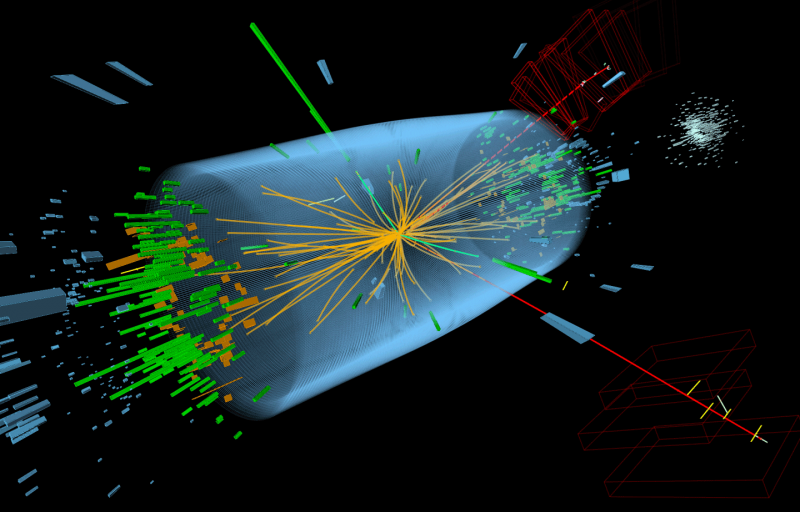
\includegraphics[scale=0.40]{Images1/large_QUxxmjstCrRXfVrLhsYBNKHMs3X1IteSRxk1ndXA-ME.png}
    \end{figure}
    \vfill
    Année académique 2019-2020
    \vfill
\end{center}

Ce document est une proposition de support de cours à destination des étudiants suivant le cours de physique subatomique, atomique et moléculaire. Il a été rédigé par les étudiants suivant ce même cours pendant l'année académique 2019-2020 et se base sur les slides mises à disposition par les professeurs, les notes de cours partagées par les étudiants ingénieurs (merci à Sofiane Arib et Pierre Laboureur) ainsi que diverses ressources externes (genre wikipédia tmtc).

\newpage
\tableofcontents

%\newpage
%\part{Introduction (Vincent Lemaître)}
%\begin{center}
%    En cas de questions ou de remarques sur cette partie : contactez Eléonore Lieffrig
%\end{center}
%\section{Introduction}
\subsection{Rappels sur les unités}
En physique atomique et subatomique, on n'utilisera pas les unités classiques que sont le \si{kg}, le \si{m}, etc., mais les unités naturelles, plus appropriées à l'échelle et aux dimensions des structures et phénomènes qui seront étudiés. L'unité de longueur est par exemple le femtomètre (\SI{e-15}{m}), ordre de grandeur du noyau atomique. De plus, on considérera, comme dans le système Heaviside-Lorentz, que  $\hbar=c=\epsilon_0=\mu_0=1$, ce qui transforme quelque peu des expressions familières comme celle de la constante de structure fine, qui devient

\[
    \alpha=\dfrac{e^2}{4\pi\epsilon_0\hbar c}=\dfrac{e^2}{4\pi}\approx\dfrac{1}{137}
\]
Une autre conséquence de cette hypothèse est illustrée dans le tableau ci-dessous: l'unité de masse, qui était précédemment une énergie par vitesse carrée,  devient une énergie, le \si{GeV} et celle de temps, quant à elle, devient l'inverse d'une énergie, le \si{GeV^{-1}}, avec $\SI{1}{GeV^{-1}}=\SI{6.59e-25}{s}$

\begin{table}[H]
    \centering
    \begin{tabu} to 0.7\textwidth {X[2.5,l]X[3.5,l]X[3,l]}
        \hspace*{-3.5mm} (a) & &\\
        \hline\hline
        Quantité & Unité dehaute énergie & Valeur en unité SI \\ \hline
        longueur & \SI{1}{fm} & \SI{e-15}{m} \\
        énergie  & $\SI{1}{GeV} = \SI{e9}{eV}$ & \SI{1.602e-10}{J} \\
        masse, $E/c^2$ & $\SI{1}{GeV}/c^2$ & \SI{1.78e-27}{kg}\\
        $\hbar = h/(2\pi)$ & \SI{6.588e-25}{GeV s} & \SI{1.055e-34}{J s}\\
        $c$ & \SI{2.998e23}{fm s^{-1}} & \SI{2.998e8}{ms^{-1}}\\
        $\hbar c$ & \SI{0.1975}{GeV fm} & \SI{3.162e-26}{J m}\\ \hline\hline \\
    \end{tabu}
    \begin{tabu} to 0.7\textwidth {XX}
        \hspace*{-3.5mm} (b) & \\
        \hline\hline
        \hspace*{-3mm} Unités naturelles; $\hbar = c = 1$ & \\
        masse, $Mc^2/c^2 $ & \SI{1}{GeV} \\
        longueur, $\hbar c/(Mc^2)$ & $\SI{1}{GeV^{-1}} = \SI{0.1975}{fm}$ \\
        temps, $\hbar c/(Mc^3)$ & $\SI{1}{GeV^{-1}} = \SI{6.59e-15}{s}$\\\hline
        \multicolumn{2}{l}{\hspace*{-3mm} Unités Lorentz-Heaviside, $\varepsilon_0 = \mu_0 = \hbar = c = 1$}\\
        constante de structure fine & $\alpha = e^2/(4\pi) \approx 1/137.06$\\\hline\hline
    \end{tabu}
    \caption{Unités naturelles}
    \label{tab:unites_naturelles}
\end{table}

\subsection{Tableau de Mendeleïev}
Le tableau de Mendeleïev (1869) représente tous les éléments chimiques, ordonnés par numéro atomique croissant et organisés en colonnes en fonction de leur configuration électronique, laquelle sous-tend leurs propriétés chimiques.  Le modèle de l'atome comportant des électrons sur des couches permet cette classification des éléments en familles, qui met en évidence la périodicité des propriétés chimiques. Par exemple, la première colonne est celle des Alcalins qui ne comportent qu'un seul électron sur la dernière couche et la dernière colonne est celle des Gaz nobles dont la dernière couche est fermée.

\begin{figure}[ht]
    \centering
    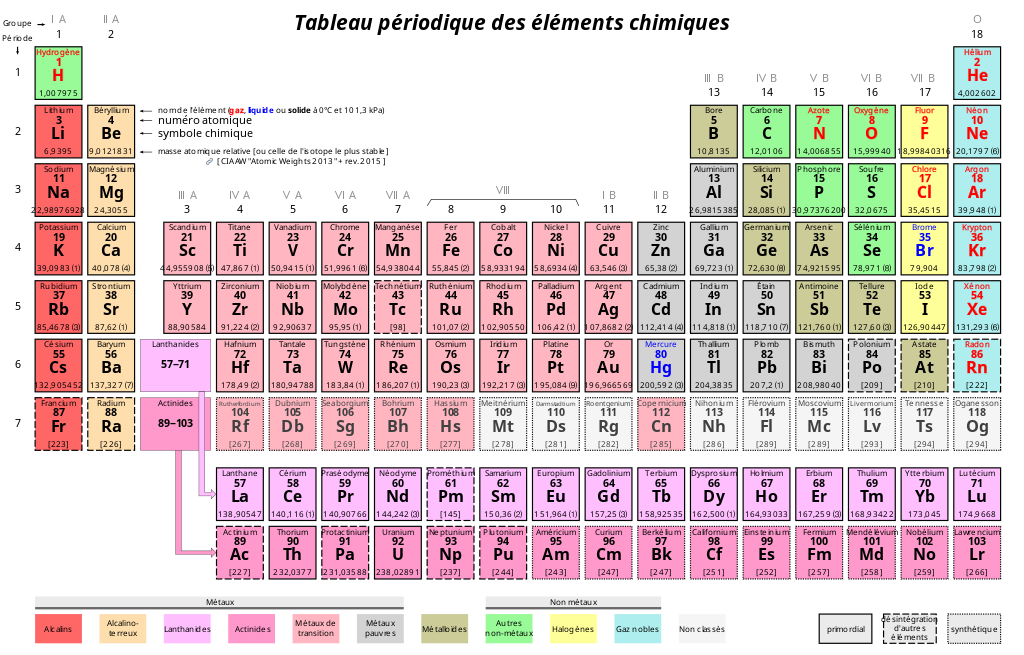
\includegraphics[scale=0.40]{Images1/mend.png}
    \caption{Tableau de Mendeleïev}
\end{figure}

Les atomes se situant dans la même période, c'est-à-dire dans la même ligne du tableau, possèdent le même nombre quantique principal n. Les éléments des mêmes groupes (i.e. même colonne) ont eux des configurations électroniques similaires et donc des propriétés chimiques similaires. On a différents groupes en fonction de la colonne: les métaux alcalins (1), les alcalino-terreux (2) ..., les halogènes (17), les gaz nobles (18). Enfin, les blocs sont des groupes d'éléments dont les électrons de valence occupent des orbitales qui partagent le même nombre quantique $l$ ($l=0,1, \dots, n-1$ correspondant à s, p, d,...).

Les éléments de ce tableau, les atomes, sont des objets très complexes dont la composition (pour le moment admise) est représentée ci-dessous, avec quelques ordres de grandeur. L'électron est un degré de liberté de l'atome, qui possède une charge et un spin, mais pas de position...

\begin{figure}[ht]
    \centering
    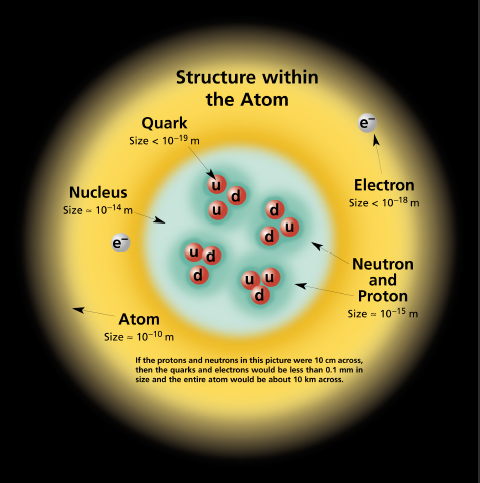
\includegraphics[scale=0.45]{Images1/atome.png}
    \caption{Structure de l'atome}
    \label{fig:struct_atome}
\end{figure}
On admet pour le moment que la matière est constituée de vide et des 4 particules suivantes:

\begin{itemize}
    \item \textbf{les quarks down}, possédant une charge électrique de -1/3
    \item \textbf{les quarks up}, possédant une charge électrique de 2/3
    \item \textbf{les électrons}, de charge -1, responsables des phénomènes électriques et des réactions chimiques
    \item \textbf{les photons}, responsables de l'interaction électromagnétique
\end{itemize}
Protons et neutrons sont composés de quarks: 1 down et 2 up pour le proton, 2 down et 1 up pour le neutron (logique).

\subsection{Modèles de la matière et liens avec la cosmologie et l'astrophysique}
La structure de la matière et l'interaction entre constituants sont intimement liées. En effet, c'est l'interaction entre les rayonnements et la matière qui autorise la description de la structure de celle-ci. Par exemple, les microscopes optiques permettent d'observer des objets de très petite taille, mais leur pouvoir de résolution (i.e leur capacité à séparer des détails très voisins) est limité par le caractère ondulatoire de la lumière, qui engendre de la diffraction. Ainsi, pour voir un objet de taille $d$, il faut un rayonnement dont la longueur d'onde associée $\lambda$ empêche la diffraction, c'est-à-dire telle que
\[ \lambda < d \]
La résolution limite pour de la lumière visible est donc de l'ordre de $\SI{0.5}{\mu m}$.

\subsubsection{Modèles de l'atome}
Différents modèles de plus en plus affinés se sont succédé pour décrire l'atome. Le modèle atomique du <<plum pudding>> fut proposé par J.J. Thomson (Fig \ref{fig:modele_thompson}), qui découvrit l'électron en 1897. Dans ce modèle, l'atome est composé d'électrons plongés dans une <<soupe>> de charges positives pour équilibrer cette charge positive, comme des prunes/raisins selon les versions dans un pudding. Les électrons ne se déplacent pas de façon aléatoire dans l'atome, mais sur des anneaux stabilisés par les interactions entre électrons.

\begin{figure}[ht]
    \centering
    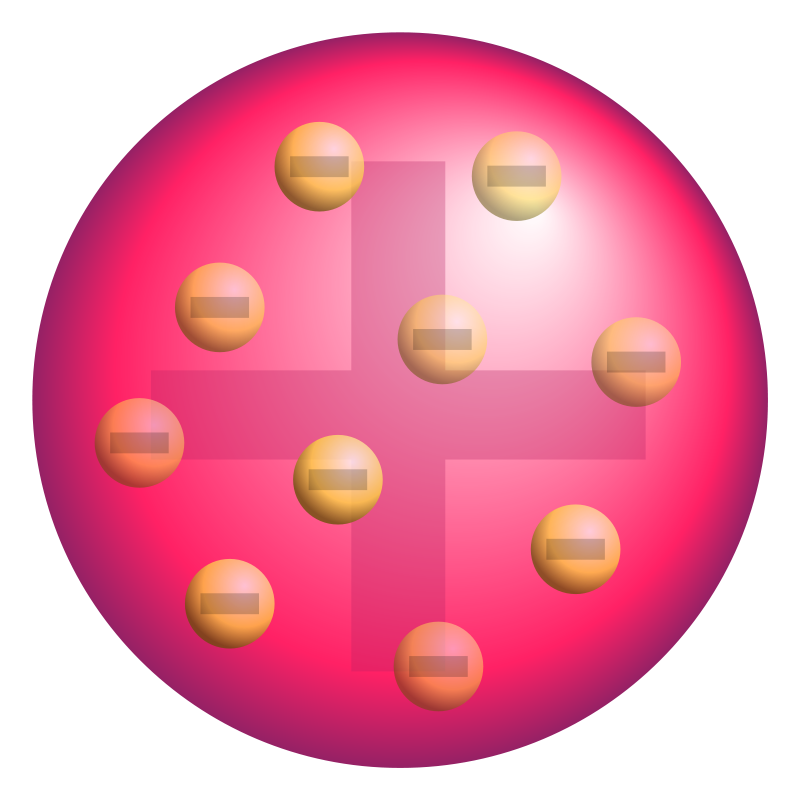
\includegraphics[scale=0.15]{Images1/thomson.png}
    \caption{Modèle de l'atome de Thomson (1897)}
    \label{fig:modele_thompson}
\end{figure}

Ernest Rutherford, considéré comme le père de la physique nucléaire, mit en évidence en 1909 l'existence du noyau atomique, ayant également prouvé au passage l'existence du proton. En 1932, Chadwick découvrit le neutron, remettant ainsi en question le modèle de l'atome. Rutherford imagine donc un atome constitué d'un noyau chargé positivement contenant la majorité de la masse de l'atome et, séparés par du vide, des électrons tournant autour de ce noyau comme des planètes autour d'une étoile (Fig \ref{fig:modele_rutherford}).

\begin{figure}[ht]
    \centering
    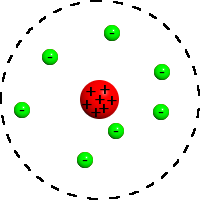
\includegraphics[scale=0.65]{Images1/modelerutherford.png}
    \caption{Modèle de l'atome de Rutherford (1909)}
    \label{fig:modele_rutherford}
\end{figure}

Les accélérateurs actuels (linéaires, circulaires (LHC)) nous permettent d'observer les plus petits constituants de la matière, mais plus la taille de ce que l'on souhaite observer est petite, plus ils doivent être grands, comme illustré ci-dessous. Sur les échelles suivantes sont également représentées les longueurs et énergies, liées par la relation de la longueur d'onde de de Broglie:
\[ \lambda=\dfrac{h}{\sqrt{2mE}} \]
En fait ici c'est un peu complexe, la vraie relation de la longueur d'onde de de Broglie c'est
\[\lambda=\dfrac{h}{p}\]
Ici la relation $p = \sqrt{2mE}$, vient de l'approximation non relativiste $E = \dfrac{p^{2}}{2m}$ (on voit déjà facilement que le cas purement relativiste de la lumière donne une longueur d'onde infinie). L'approximation reste malgré tout correcte assez longtemps (par exemple $v = c/10$ n'est pas du tout relativiste). Selon Lemaître la distinction de régime relativiste doit être faite lorsque l'énergie cinétique commence à être de l'ordre du terme de masse\footnote{Pour rappel, $E = E_\text{cin} + mc^2 = \gamma mc^2$}. Ce terme de masse dépend uniquement de la particule que l'on traite, pour un proton c'est $\SI{938}{MeV}/c^2$ , mais pour un muon c'est $\SI{105.66}{MeV}/c^2$ et un électron c'est 207 fois moins : $\SI{511}{keV}/c^2$. Donc, attention à la formule lorsqu'on dépasse \SI{100}{MeV} pour un proton.

\begin{figure}[ht]
    \centering
    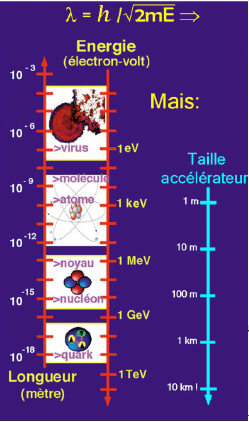
\includegraphics[scale=0.75]{Images1/echelles.png}
    \caption{Relation entre longueur et énergie}
    \label{fig:longeur_energie}
\end{figure}

\subsubsection{Connexion à la cosmologie}
Comprendre les interactions, c'est comprendre l'évolution, du Big Bang à l'apparition de la vie, soit faire de la cosmologie. La théorie du Big Bang de Lemaître et son hypothèse de l'atome primitif ont permis d'établir un lien entre l'infiniment petit (instant juste après le BB) et l'infiniment grand (l'Univers actuel).  Le rayonnement cosmique, la nucléosynthèse primordiale et l'expansion de l'Univers sont des éléments de preuve en faveur de cette théorie.

\begin{figure}[ht]
    \centering
    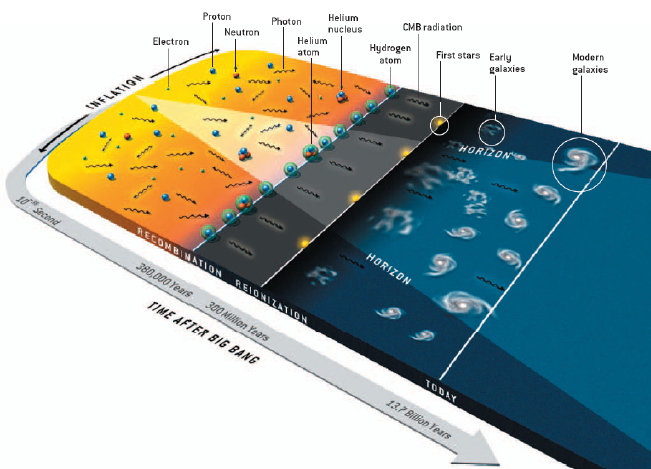
\includegraphics[scale=0.65]{Images1/univers.png}
    \caption{Évolution cosmique}
    \label{fig:evolution_cosmos}
\end{figure}

La ligne du temps de la figure \ref{fig:evolution_cosmos} représente l'évolution de l'Univers depuis le Big Bang. Pendant la première période, on est en présence d'un plasma chaud de gaz ionisé qui se refroidit petit à petit, au fur et à mesure que la nucléosynthèse primordiale se déroule. Elle s'est manifestée à l'échelle de l'Univers tout entier durant les premières dizaines de minutes suivant le Big Bang et est responsable de la formation des noyaux légers, principalement l'hélium 4, mais également le deutérium, une petite partie du lithium et des traces de béryllium. Aucun élément plus lourd n'a été créé durant cette période. Il y a juste déionisation de l'univers, car des atomes se forment.

On remarque ensuite une zone grise entre 380 000 ans et 300 000 millions d'années pendant laquelle l'Univers était <<éteint>>, c'est-à-dire neutre et opaque, il ne se passe rien à part les effets de la gravitation. Remarque: on ne sait pas encore vraiment comment se sont formés les éléments très lourds, car leur synthèse nécessite des conditions très particulières.

Après la période <<d'extinction>>, il y eut formation d'hydrogène et émission de lumière sous forme d'ondes radio, qui ont été détectées par des ingénieurs via des antennes en 1932. On note également le début de la formation des galaxies et des quasars.

Après 1 milliard d'années, l'Univers redevient <<transparent>>, la réionisation est complète,  beaucoup plus d'éléments du tableau périodique sont formés ; les galaxies évoluent. La réionisation a lieu, car les premières étoiles étaient très chaudes, à tel point qu'elles émettent dans l'UV, ce qui peut ioniser les atomes. On assiste à la formation du système solaire vers 9 milliards d'années.\\

On s'intéresse à présent aux premières minutes après le Big Bang au niveau des particules:
\begin{itemize}
    \item $t_0$: instant du Big Bang
    \item $t_0 + \SI{e-34}{s}$: compliqué, relève de la théorie des cordes et de la gravité quantique à boucles.
    \item $t_0 + \SI{e-12}{s}$: énergie de \SI{1}{TeV}, soupe de particules élémentaires (bosons W, quarks en tout genre, muons, positrons...). Il y a une légère asymétrie entre matière et antimatière, qui n'est toujours pas comprise à l'heure actuelle. Un peu après, il ne reste plus assez d'énergie pour créer une paire quark-antiquark, il reste donc quelques quarks tout seuls.
\end{itemize}

\begin{figure}[ht]
    \centering
    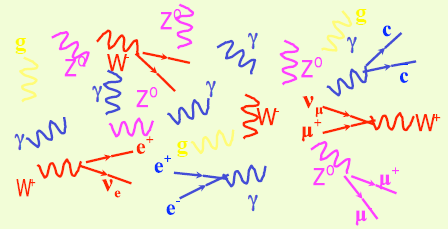
\includegraphics[width=0.45\textwidth]{Images1/soupe.png}
    \caption{Soupe primordiale}
    \label{fig:soupe_promordiale}
\end{figure}

\begin{rem}
    Comment peut-on affirmer avec certitude qu'il n'existe pas d'anti-monde rempli d'antimatière (une anti-galaxie avec un anti-soleil, etc.) ? Car il provoquerait des effets gravitationnels et électromagnétiques tellement cataclysmiques qu'on ne pourrait pas les rater.
\end{rem}

\begin{itemize}
    \item $t_0 + \SI{e-2}{s}$: énergie de \SI{1}{GeV}, mariage des quarks et formation des nucléons sous l'effet de l'interaction forte (neutron = 2 down + 1 up, proton = 2 up + 1 down)
    \item $t_0+ \SI{100}{s}$: \SI{100}{eV} ($10^9$ degrés), existence d'états liés entre neutrons et protons sous l'effet de l'interaction faible, comme le deutérium et l'hélium (noyaux légers).
\end{itemize}

\begin{figure}[ht]
    \centering
    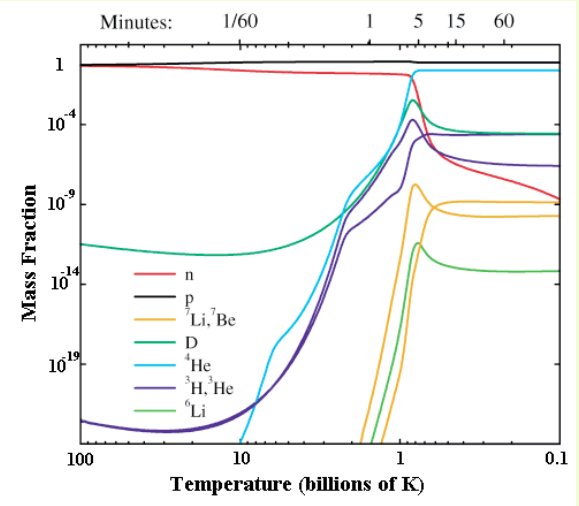
\includegraphics[scale=0.50]{Images1/tempmass.png}
    \caption{Évolution des proportions d'éléments en fonction du temps}
\end{figure}

\begin{itemize}
    \item $t_0+30$ min: le contenu de l'Univers est dominé par les protons et l'hélium (il y a aussi des électrons et photons). On est en présence d'un plasma électriquement neutre (Fig. \ref{fig:BB_30mn}).
    \item $t_0 + 300.000$ ans: les photons sont libres, on les observe
    \item $t_0 + 700.000$ ans: 3000 degrés, formation des atomes les plus simples sous l'effet de l'interaction électromagnétique
\end{itemize}

\begin{figure}[ht]
    \centering
    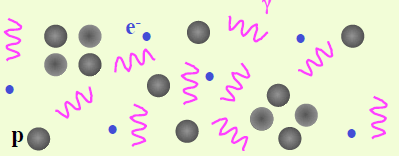
\includegraphics[scale=0.50]{Images1/30min.png}
    \caption{Univers 30 minutes après le Big Bang}
    \label{fig:BB_30mn}
\end{figure}

% \textcolor{blue}{[Revoir cette section]}
\subsubsection{Connexion à l'astrophysique}
En ce qui concerne la connexion à l'astrophysique, la structure microscopique de la matière permet une compréhension très riche des astres et du cosmos.

Par exemple le Nuage d'Orion est relativement proche de la Terre dans la Voie lactée. L'observation de son spectre permet de conclure sur sa composition en certains atomes et molécules. De telles conclusions ne seraient pas possibles sans la connaissance du monde microscopique pour décrypter ces observations.


\section{Structure de la matière}
Cette section porte sur la découverte de particules et de rayonnements, ainsi que sur leurs pertes d'énergie. Il est donc bon de commencer par restituer différents évènements sur une ligne du temps (Fig. \ref{fig:decouvertes}):

\begin{figure}[ht]
    \centering
    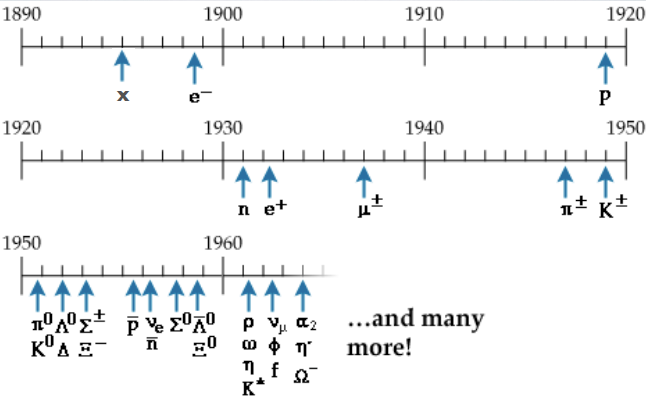
\includegraphics[scale=0.50]{Images1/ldt.png}
    \caption{Découverte de différentes particules et rayonnements}
    \label{fig:decouvertes}
\end{figure}

\begin{itemize}
    \item 1895: Découverte des rayons X (Roentgen)
    \item 1896: Découverte de la radioactivité (Becquerel)
    \item 1897: Découverte de l'électron (J.J. Thomson)
    \item 1909: Preuve que les particules $\alpha$ sont de noyaux d'hélium (Rutherford)
    \item 1911: Découverte du noyau (Rutherford)
    \item 1912: Découverte des rayonnements cosmiques (Hess)
    \item 1928: Théorie de l'$\alpha$-radioactivité (Gamow, Gurney, Condon)
    \item 1930: Hypothèse du neutrino (Pauli)
    \item 1932: Découverte du neutron (Chadwick)
    \item 1934: Théorie de la $\beta$-radioactivité (Fermi)
    \item ...
\end{itemize}


\subsection{Des rayons X à la découverte de l'électron}
\subsubsection{Fluorescence et phosphorescence}
Une molécule fluorescente possède la propriété d'absorber de l'énergie lumineuse (lumière d'excitation) et de la restituer rapidement sous forme de lumière fluorescente (lumière d'émission). Une fois l'énergie du photon absorbée, la molécule se trouve alors généralement dans un état électroniquement excité, souvent un état singulet, noté S1. (L'état fondamental qui est aussi singulet est noté S0.) Le retour à l'état fondamental peut alors se faire de différentes manières : soit par fluorescence, soit par phosphorescence (Fig. \ref{fig:fluorescence_phosphorescence}).

La fluorescence est caractérisée par l'émission d'un photon de manière très rapide. Cette rapidité s'explique par le fait que l'émission respecte une des règles de sélection de l'émission de photons de la mécanique quantique qui est $\Delta S=0$, ce qui signifie que la molécule reste dans un état singulet.

La phosphorescence quant à elle est caractérisée par une transition d'un état S=0 vers un état S=1 (état triplet noté T1), qui n'est pas permise par le modèle quantique, mais qui est rendue possible par le couplage spin-orbite. Cependant, la transition est plus lente à s'effectuer. Suit alors une émission de photon pour retourner à l'état fondamental.

\begin{figure}[ht]
    \centering
    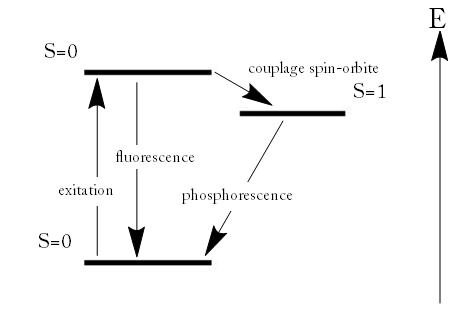
\includegraphics[scale=0.65]{Images1/fluophospho.jpg}
    \caption{Fluorescence VS phosphorescence}
    \label{fig:fluorescence_phosphorescence}
\end{figure}

\subsubsection{Découverte des rayons X (Röntgen, 1895, PN en 1901)}
Les rayons X sont une forme de rayonnement électromagnétique à haute fréquence constitué de photons. L'énergie de ces photons va d'une centaine d'$eV$ à environ un $\si{MeV}$. Anecdote: Röntgen les a appelés rayons <<X>> en référence à l'inconnue mathématique.

Ils sont de même nature que les rayons gamma, mais produits différemment : les rayons X sont produits par des transitions électroniques alors que les rayons gamma proviennent de la désintégration radioactive des noyaux des atomes.

Comment Röntgen les a-t-il découverts? Comme beaucoup de physiciens à l'époque, il se passionnait pour les <<rayons cathodiques>>, étudiés auparavant par William Crookes via les célèbres <<tubes de Crookes>>.

\begin{figure}[ht]
    \centering
    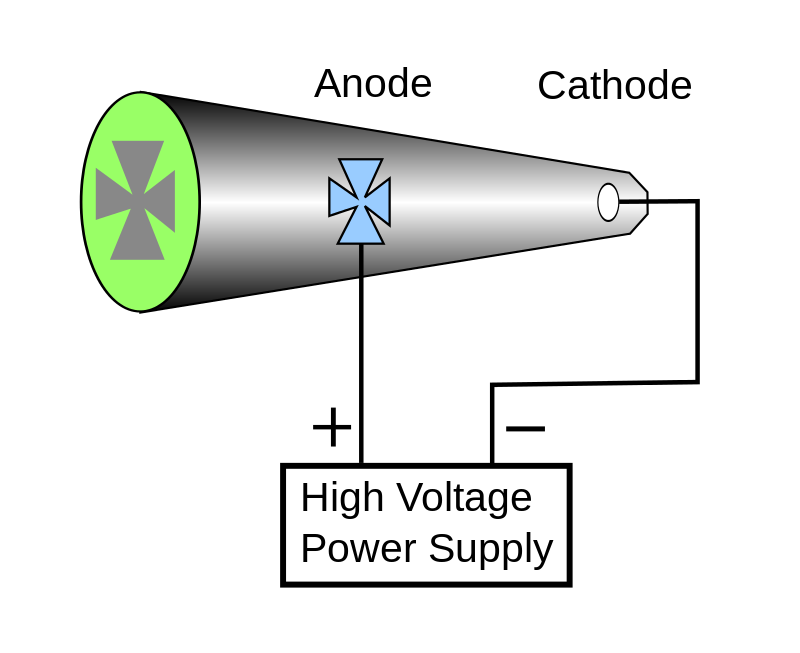
\includegraphics[scale=0.20]{Images1/tubecrookes.png}
    \caption{Schéma d'un tube de Crookes}
\end{figure}

Le tube de Crookes est un tube de verre froid sous vide partiel possédant 2 électrodes de métal, une à chaque extrémité. Quand on applique une forte tension électrique entre les électrodes, le champ électrique induit l'accélération des ions chargés présents dans le gaz résiduel. Ils entrent en collision avec les autres molécules du gaz, leur arrachant au passage des électrons, ce qui crée des cations. Ces derniers sont attirés par la cathode (électrode négative). À l'instant où ils la percutent, ils éjectent un grand nombre d'électrons de la surface métallique, qui sont eux attirés par l'électrode positive, l'anode. Ces électrons sont ce qu'on a appelé plus haut les <<rayons cathodiques>>. Il y a donc un faisceau d'électrons qui traverse le tube depuis la cathode vers l'anode.

Quand on applique une différence de potentiel supérieure ou égale à \SI{5 000}{V} à un tube de Crookes, les électrons sont accélérés à une vitesse telle qu'un rayonnement est émis de l'anode vers le récepteur. Le spectre de ce rayonnement est continu et comporte des pics. Il montre 2 caractéristiques témoignant de 2 phénomènes différents:

\begin{itemize}
    \item \textbf{Le rayonnement continu de freinage (ou Bremsstrahlung)} : les électrons accélérés émettent des rayons X au moment où ils passent à proximité de la charge électrique portée par le noyau atomique des molécules composant la cible et que leur trajectoire est brutalement infléchie. (car ils sont décéléré par le champ électrique des noyaux)
    \item \textbf{la fluorescence X} : quand les électrons rencontrent les <<électrons profonds>> d'un atome de la paroi du tube, ils les placent dans des niveaux d'énergie plus élevés, car ils leur arrachent des électrons sur la couche externe. Les électrons de l'atome doivent alors redescendre d'un niveau d'énergie pour se stabiliser, émettant au passage des rayons X.
\end{itemize}

En 1895, Röntgen manipulait un tube de Crookes recouvert d'un carton noir quand il s'aperçut qu'un des écrans scintillants situé à proximité du tube scintillait un peu. Il en déduit que les rayons issus du tube étaient capables de traverser le carton et faire fluorescer l'écran, même dans l'obscurité. Il observa aussi que les rayons traversaient ses livres et papiers, mais qu'il était plus ou moins pénétrant en fonction de la densité de l'objet à traverser. \\

Aujourd'hui, on produit les rayons X dans des tubes spéciaux (tubes à rayons X figure \ref{fig:tube_rayon_x}) qui sont en quelque sorte une évolution des tubes de Crookes. Contrairement à ces derniers, ils sont chauffés. Une haute tension est établie entre deux électrodes. Il se produit alors un courant d'électrons de la cathode vers l'anode comme expliqué plus haut. Les électrons sont freinés par les atomes de la cible, ce qui provoque un rayonnement continu de freinage ou Bremsstrahlung, dont une partie du spectre est dans le domaine des rayons X. Ces électrons excitent les atomes de la cible, et ceux-ci réémettent un rayonnement X caractéristique par le phénomène de fluorescence X. Le spectre sortant du tube est donc la superposition du rayonnement de freinage et de la fluorescence X de la cible (voir figure \ref{fig:spectre_rayon_x}). Le système représenté en bleu sur le schéma ci-dessous est un dispositif de circulation d'eau pour refroidie le tube, car la dissipation de chaleur est énorme, bien qu'aujourd'hui cet effet soit mieux contrôlé, notamment en faisant tourner l'anode pour qu'elle ne soit pas toujours percutée au même endroit. La bobine est souvent en tungstène.

\begin{figure}[ht]
    \centering
    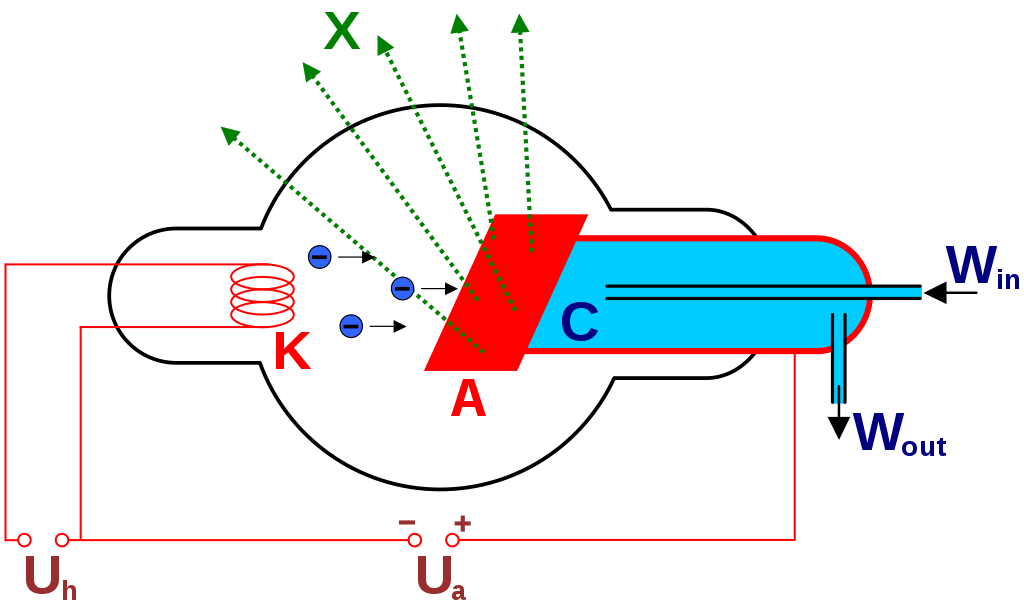
\includegraphics[width=0.5\textwidth]{Images1/rayonsxtube.png}
    \caption{Production de rayons X dans un tube à anode fixe}
    \label{fig:tube_rayon_x}
\end{figure}

\begin{figure}[ht]
    \centering
    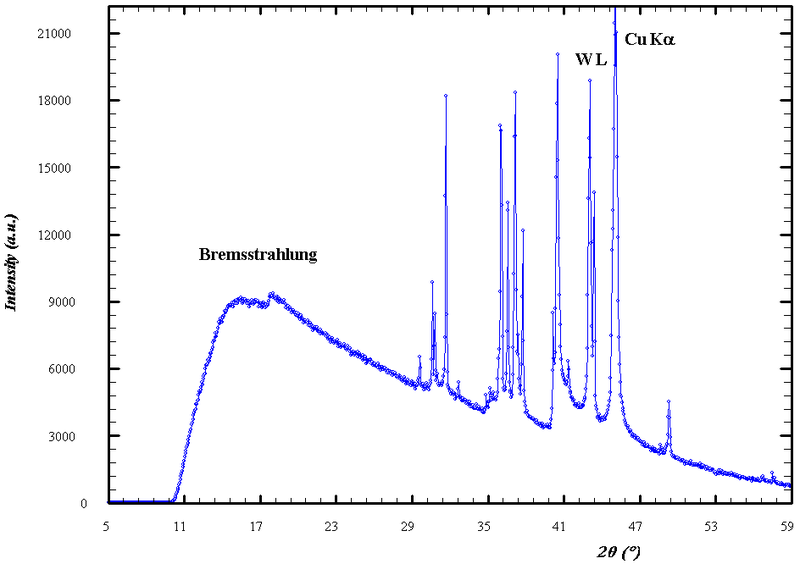
\includegraphics[scale=0.30]{Images1/rayonnement.PNG}
    \caption{Composition du spectre sortant du tube à rayons X}
    \label{fig:spectre_rayon_x}
\end{figure}

\subsubsection{Découverte de la radioactivité naturelle (Becquerel, 1896, PN en 1903)}
En 1896, Henri Becquerel cherche à déterminer si le phénomène de fluorescence des sels d'uranium est de même nature que les rayons X. Il dépose des sels phosphorescents d'uranium sur des plaques photographiques, elles-mêmes enveloppées dans du papier noir et les expose au soleil. Les photographies révèlent l'image des cristaux de sel d'uranium. Becquerel pense donc que l'énergie du soleil est absorbée par l'uranium avant d'être réémise sous forme de rayons X.

Cependant, un jour de mauvais temps, Becquerel doit renoncer à reproduire son expérience et il range donc ses plaques photographiques imprégnées de sels d'uranium dans un placard. Surprise, quelques jours plus tard, les plaques sont quand même impressionnées et Becquerel distingue même l'image négative d'une croix de cuivre qui se trouvait entre l'uranium et l'une de ses plaques photographiques. Il ne peut donc que conclure qu'une substance inerte se montre capable d'émettre des rayons, en l'absence de lumière, qui traversent le papier, mais sont tout de même arrêtés par le métal. \\

On a une loi de comportement pour décrire la désintégration radioactive: dans une boîte avec $N$ particules, le taux de désintégration ne change pas. C'est assez contre-intuitif par rapport à la nature, car si on fait une analogie avec notre classe, dans 50 ans, quelques-uns auront disparu à cause du vieillissement, mais ce nombre de disparus sera encore bien plus important dans 100 ans (rip). \textbf{Cette notion de vieillissement n'existe pas chez les particules}, elles se désintègrent au même taux à tout moment:
\[    \Delta N(t)=-\lambda N(t) \Delta t    \]
où
\begin{itemize}
    \item $N(t)$ est le nombre de noyaux radioactifs de l'espèce initiale existant à l'instant $t$. On suppose qu'il ne varie que très peu dans l'intervalle de temps $[t,t+\Delta t]$
    \item $\Delta N(t)$ est le nombre de noyaux qui se transforment pendant l'intervalle de temps $[t,t+\Delta t]$
    \item $\lambda$ est une constante de proportionnalité ayant les dimensions de l'inverse d'un temps, appelée constante radioactive (remarquons qu'elle ne dépend pas du temps: les atomes ne vieillissent pas)
\end{itemize}
On a donc
\[
    \fdif{N(t)}{t}=-\lambda N(t)
\]
ou encore
\[
    N(t)=N(0)e^{-\lambda t}
\]
N.B: une fois qu'ils ont découvert la radioactivité et ses <<pouvoirs curatifs miraculeux>>, les gens se sont un peu emballés...

\begin{figure}[H]
    \centering
    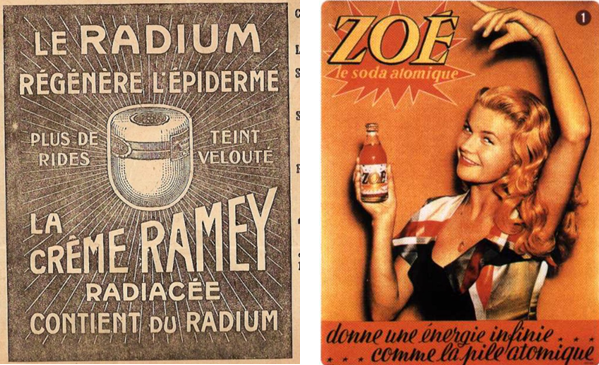
\includegraphics[scale=0.60]{Images1/produits.png}
    \caption{Crème et soda radioactifs}
\end{figure}

\subsubsection{Découverte de l'électron (Thomson, 1897, PN en 1906)}
Les tubes de Crookes furent utilisés dans de très nombreuses expériences afin de déterminer la nature des rayons cathodiques. Deux théories coexistaient : Crookes croyait qu'il s'agissait de <<corpuscules>> ou <<matière radiante>> c'est-à-dire d'atomes chargés électriquement. D'autres chercheurs pensaient qu'il s'agissait de vibrations de l'éther, une nouvelle forme de rayonnement électromagnétique. Le débat continua jusqu'à ce que J. J. Thomson mesure leur masse, prouvant qu'ils avaient affaire à des particules chargées négativement inconnues auparavant, qu'il appela <<corpuscules>>, mais qui furent plus tard appelées électrons. En 1869, on construisit une anode avec une forme de croix de Malte dans le tube. Lorsque le tube était allumé, il projetait une ombre en forme de croix sur la matière fluorescente dans la partie arrière du tube (figure \ref{fig:croix_de_malte}), montrant que les rayons se déplaçaient en ligne droite.

\begin{figure}[ht]
    \centering
    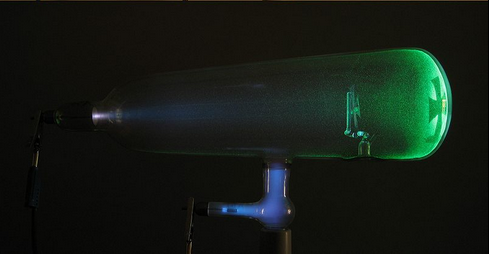
\includegraphics[scale=0.60]{Images1/croixmalte.PNG}
    \caption{Expérience de la croix de Malte}
    \label{fig:croix_de_malte}
\end{figure}

La preuve expérimentale de l'existence des électrons est le résultat de 3 expériences menées par Thomson:

\begin{itemize}
    \item Première expérience: Il cherche à savoir si on peut séparer la charge négative des rayons cathodiques par le biais du magnétisme. La conclusion est que ce n'est pas le cas. (d'où <<interprétation corpusculaire des rayons cathodiques>>)
    \item Deuxième expérience: Il prouve que les rayons cathodiques peuvent être déviés par un champ électrique. Il construit un tube cathodique muni d'une couche de peinture phosphorescente au bout pour détecter des rayons incidents. Thomson démontre une déviation dans un sens, qui indique que la charge des rayons cathodiques est négative. (Fig. \ref{fig:thompson_exp_2})

    \begin{figure}[ht]
        \centering
        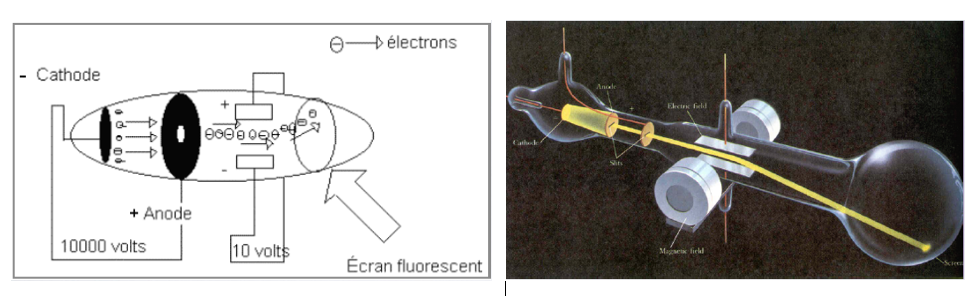
\includegraphics[scale=0.60]{Images1/2eexpthomson.PNG}
        \caption{Deuxième expérience de Thomson - Dispositif expérimental}
        \label{fig:thompson_exp_2}
    \end{figure}

    \item Troisième expérience: Détermination du rapport charge/masse $(e/m)$. Pour déterminer ce rapport, Thomson mesure la déviation et l'énergie cinétique des rayons cathodiques sous l'influence du champ magnétique. Son calcul lui donne un résultat pour $e/m$ mille fois plus élevé que le rapport analogue pour un ion hydrogène, ce qui suggère que les rayons cathodiques contiennent des particules soit très légères soit très hautement chargées. Thomson arrive à la conclusion que les rayons cathodiques sont composés de <<corpuscules>> qui proviennent de l'intérieur des atomes des électrodes, ce qui implique que les atomes sont divisibles. Le <<corpuscule>> découvert par Thomson est l'électron.
    S'en suit la proposition de modèle du <<plum pudding>> pour l'atome.
\end{itemize}

\subsubsection{Détermination de la charge de l'électron}
Elle se fit via l'expérience de la goutte d'huile de Millikan, qui consiste à pulvériser de minuscules gouttes d'huiles électrisées entre les 2 électrodes horizontales d'un condensateur plan chargé. Les gouttes sont soumises à plusieurs forces qui s'équilibrent rapidement, elles se déplacent donc à une vitesse constante qu'on peut mesurer.

\begin{figure}[ht]
    \centering
    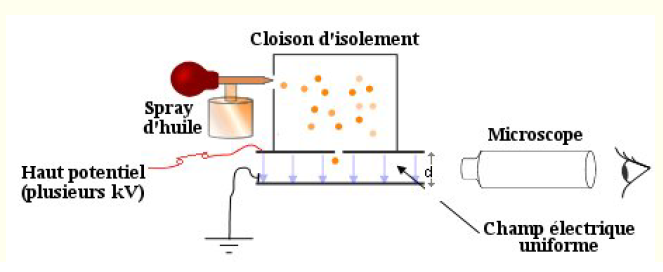
\includegraphics[scale=0.60]{Images1/millikan.PNG}
    \caption{Expérience de la goutte d'huile de Millikan}
\end{figure}

Le principe est de sélectionner une goutte, et  d'analyser son mouvement sous l'action des forces agissant sur elle  à différentes valeurs d'ionisation.

Millikan, mesura la vitesse d'une gouttelette d'huile qu'il ionisait en l'irradiant grâce à des rayons X. Cette mesure de la vitesse fut déterminée par le rapport entre la distance parcourue par la gouttelette d'huile et le temps mis pour effectuer ce déplacement. Ses observations lui firent se rendre compte que toutes les valeurs d'ionisation étaient multiples entiers de $e=\SI{1.592e-19}{C}$, que l'on définit comme la charge élémentaire.

\paragraph{Détails:} Si on modélise simplement le problème, la goutte d'huile subit les 4 forces suivantes:
\begin{itemize}
    \item Son poids $\Vec{P}=\dfrac{4}{3}\pi r^3 \rho_h\Vec{g}$
    \item La force électrostatique $\Vec{F_E}=q\Vec{E}$
    \item La poussée d'Archimède $\Vec{F_A}=-\dfrac{4}{3}\pi r^3 \rho_a \Vec{g}$
    \item La force de trainée (résistance de l'air) $\Vec{F_R}=-6\pi\eta r\Vec{v}$ où $\eta$ est le coefficient de viscosité de l'air et $v$ la vitesse de la gouttelette.
\end{itemize}
On peut mesurer la charge $q$ de la goutte de différentes façons. Considérons la méthode du champ constant, dans laquelle on garde l'amplitude du champ constante et on alterne la polarité du condensateur, de sorte que la force électrique soit dirigée tantôt vers le haut, tantôt vers le bas. \\[0,2cm]
Dans le cas de la force électrique vers le haut (vitesse $v_1$), on a
\begin{equation}
    qE+F_A = mg+6\pi\eta rv_1
    \label{eq:force_elec_haut}
\end{equation}
    Pour la force électrique vers le bas (vitesse $v_2$),
\begin{equation}
    qE+mg = 6\pi\eta rv_2 + F_A
    \label{eq:force_elec_bas}
\end{equation}
Si on soustrait (\ref{eq:force_elec_haut}) et (\ref{eq:force_elec_bas})
\[
    2(mg-F_A)=6\pi\eta r(v_2-v_1)
\]
vu que

\[
mg-F_A=\dfrac{4\pi}{3}r^3g(\rho_h-\rho_a)\quad\text{et}\quad
r=\dfrac{3}{2}\sqrt{\dfrac{\eta(v_2-v_1)}{g(\rho_h-\rho_a)}}
\]
Si on additionne (\ref{eq:force_elec_haut}) et (\ref{eq:force_elec_bas}), on obtient
\[
    2qE=6\pi\eta r(v_2+v_1)
\]
donc
\[
    q=\dfrac{9\pi}{2E}\sqrt{\dfrac{\eta^3(v_2-v_1)}{g(\rho_h-\rho_a)}}(v_2+v_1)
\]
Si on effectue 2 mesures de vitesse pour une goutte donnée, on peut donc déterminer $q$.

\subsection{Perte d'énergie dans la matière}

L'intérêt de l'étude de la perte d'énergie lors d'une interaction particule-matière réside dans le fait que c'est l'outil principal de détection de particule. Commençons par étudier la perte d'énergie des particules lourdes, c'est-à-dire des particules possédant une masse bien supérieure à celle de l'électron. Si elles ont une énergie basse, la perte d'énergie est dominée par leur interaction électromagnétique avec les électrons atomiques: il y a excitation et/ou ionisation de l'atome par transfert d'une partie de l'énergie cinétique de la particule incidente. Si au contraire elles ont une haute énergie, ce sont les interactions nucléaires qui sont importantes.

\subsubsection{Perte d'énergie par ionisation}
La section efficace (cfr section \ref{sec:section_efficace}) étant très petite (de l'ordre de \SI{e-17}{cm^2}), la probabilité de collision est très faible, mais la grande densité d'atomes ($N_A=\SI{6.02e23}{\mole^-1}$) dans un matériau rend la perte d'énergie totale très importante, même pour une faible épaisseur. Par exemple, un proton de 10 \si{MeV} perd toute son énergie dans \SI{0.25}{mm} de cuivre !

L'énergie est perdue par la particule dans des <<collisions inélastiques>> avec les électrons des atomes du matériau. On a un très grand nombre de collisions, par conséquent l'énergie perdue par collision est petite. On dit qu'on a affaire à une diminution \textbf{continue} d'énergie. À la fin du parcours, les électrons sont capturés par la particule jusqu'à ce que l'énergie de cette dernière soit de l'ordre de l'énergie thermique des atomes du milieu.

\begin{rem}
    Le phénomène est décrit à l'aide du terme collision, mais il n'y a pas nécessairement contact entre l'électron incident (ou la particule chargée) et l'électron de l'atome cible. Néanmoins, le phénomène résultant de cette interaction électrostatique de durée très brève peut s'apparenter à une collision.
\end{rem}

Calculons la perte d'énergie se faisant lors du passage à travers une couche $\dif x$ de matière, comme représenté sur la figure \ref{fig:interraction_particule_matiere}.
\begin{figure}[ht]
    \centering
    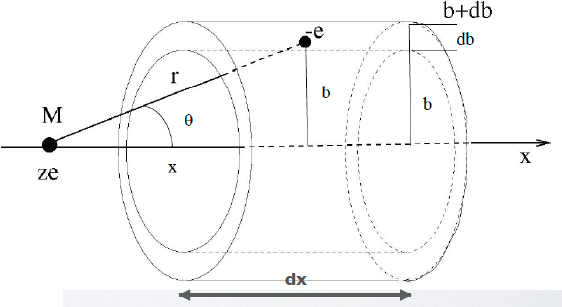
\includegraphics[scale=0.60]{Images1/pertenrj.PNG}
    \caption{Interaction entre particule (ze) et électron de matière}
    \label{fig:interraction_particule_matiere}
\end{figure}
L'impulsion verticale fournie par la particule incidente à un électron atomique à travers la force de Coulomb est
\[
    \Delta P_t=\int_{-\infty}^\infty F_y \dt=\int_{-\infty}^\infty \dfrac{ze^2}{4\pi \epsilon_0 r^2} \sin{\theta}\dfrac{\dif x}{v}
\]
où
\[\begin{cases}
    \dfrac{1}{r^2} &= \dfrac{\sin^2\theta}{b^2} \\[2mm]
    x &= \dfrac{b}{\tan{\theta}} \\[2mm]
    \dif x &= -\dfrac{b}{(\sin{\theta})^2}\dif\theta
\end{cases}\]
Ainsi
\[
    \Delta P_t=\int_{0}^\pi \dfrac{ze^2}{4\pi \epsilon_0}\dfrac{\sin{\theta}}{vb}\dif\theta = \dfrac{ze^2}{2\pi \epsilon_0 vb}
\]
Dans une approche non relativiste, l'énergie transmise à l'électron est
\[
    \dif E_E=\dfrac{p^2}{2m_e}=\dfrac{z^2e^4}{8\pi^2{\epsilon_0}^2v^2b^2m_e}
\]
En admettant une distribution uniforme des électrons, le nombre de <<collisions>> que la particule subit avec des électrons situés à un paramètre d'impact compris entre $b$ et $b+\dif b$ dans une épaisseur $\dif x$ est\footnote{$A$ est la masse molaire, $\dfrac{\rho N_A}{A}$ est donc le nombre d'atomes du milieu par unité de volume.}
\[
    \dif N_e=\dfrac{\rho N_A}{A}Z(2\pi b \dif b \dif x)
\]
qui engendre un transfert d'énergie
\[
    \dif T_e=\dif N_e\dif E_e=\dfrac{z^2e^4}{4\pi \epsilon_0^2v^2bm_e}\Big(\dfrac{\rho N_A}{A}\Big)Z \dif b \dif x
\]
Par unité de distance, on a donc la perte d'énergie
\[
    -\fdif{E}{x}=\int_{b_\text{min}}^{b_\text{max}} \fdif{T_e(b)}{x}=\Big(\dfrac{\rho N_A}{A}\Big)Z\dfrac{z^2e^4}{4\pi \epsilon_0^2m_ev^2}\ln{\Big(\dfrac{b_\text{max}}{b_\text{min}}\Big)}
\]
Cependant, on a un problème puisque cette intégrale diverge. On doit donc en limiter les bornes en utilisant des arguments qualitatifs à savoir les estimations de $b_\text{min}$ et $b_\text{max}$:

\begin{itemize}[label=$\rightarrow$]
    \item \underline{\textbf{b grand $\Leftrightarrow\Delta E(b)$ petit}}\\[0,2cm]
    Les électrons sont liés aux noyaux. Le transfert d'énergie est plus petit que l'énergie moyenne d'ionisation $I$ des électrons et le processus n'est plus efficace. On imposera donc que $\Delta E(b) > I$, ce qui donne
    \[
        \dif E_e=\dfrac{1}{(4\pi \epsilon_0)^2}.\dfrac{2z^2e^4}{b_\text{max}^2v^2m_e}=I
    \]
    \item \underline{\textbf{b petit $\Longleftrightarrow\Delta E(b)$ grand}}\\[0,2cm]
    L'énergie maximale transférable est
    \[
        \Delta E_\text{max}=T_{e,max}=\dfrac{2m_e\beta^2\gamma^2c^2}{1+\left(\dfrac{m_e}{m_0}\right)^2+2\cdot\dfrac{m_e\gamma}{m_0}}
    \]
    où $m_0$ est la masse de la particule incidente.
\end{itemize}
La perte d'énergie par ionisation est donc de la forme
\[
    \dfrac{1}{\rho}\fdif{E}{x} \sim K\dfrac{z^2}{\beta^2}\dfrac{Z}{A}  \ln{\left(\dfrac{T_\text{max}}{I}\right)}
\]

On peut détecter le dépôt d'énergie au moyen de techniques telles que l'émulsion photographique, la chambre à brouillards, la chambre à bulles, le scintillateur, la détection du rayonnement Cerenkov...
On peut voir dans la figure \ref{fig:perte_energie} et \ref{fig:pertes_ionisation} que la première partie de la courbe descend assez fort, la particule rayonne beaucoup.

\begin{figure}[ht]
    \centering
    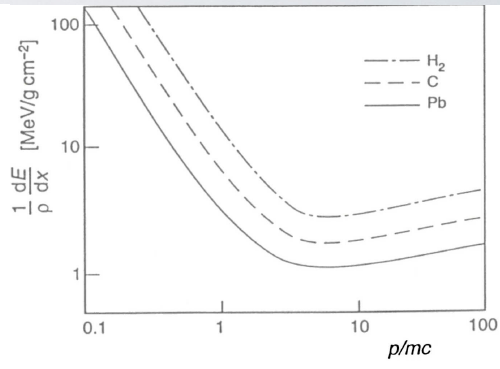
\includegraphics[scale=0.60]{Images1/perteenergie.PNG}
    \caption{Perte d'énergie par ionisation de quelques éléments}
    \label{fig:perte_energie}
\end{figure}

Un calcul plus précis, tenant compte des effets relativistes, et des corrections de densité de charge $\delta$ et $\dfrac{C}{Z}$, a été réalisé par Bethe et Block, et donne:
\[
    -\dfrac{1}{\rho}\fdif{E}{x} = K\dfrac{z^2}{\beta^2}\dfrac{Z}{A} \left[\ln\left(\dfrac{2m_ec^2\beta^2\gamma^2}{I}\right) - \beta^2-\dfrac{\delta}{2} -\dfrac{C}{Z}\right]
\]
où $K=\SI{0.307075}{MeV~g^{-1}~cm^2}$.

\begin{itemize}[label=$\longrightarrow$]
    \item \textbf{La correction de densité de charge} $\delta$ est due au fait que le champ électrique de la particule incidente polarise les atomes près de sa trajectoire. Cette polarisation réduit l'effet du champ électrique sur les électrons les plus éloignés (effet d'écran). Cela réduit la perte d'énergie. Cet effet est plus important si l'énergie des particules augmente (car le champ électrique est plus étendu), ou si la densité du matériau est plus élevée.
    \item \textbf{La correction $\dfrac{C}{Z}$} tient compte des effets de liaison des électrons et est importante à basse énergie.
\end{itemize}

\begin{rem}
    Cette formule met bien en évidence les dépendances de $\fdif{E}{x}$: le terme en $\dfrac{z^2}{\beta^2}$ montre la dépendance en la particule incidente (exemple: une particule $\alpha$ perd 4 fois plus d'énergie qu'un proton, pour un même $\beta$ et un même milieu), et celui en $\dfrac{Z}{A}$ montre la dépendance du milieu.
\end{rem}
\begin{rem}
    La relation entre $\fdif{E}{x}$ et la profondeur de pénétration est appelée courbe de Bragg. La dépendance en $1/v^2$ est marquée par la présence d'un pic appelé pic de Bragg (Figure \ref{fig:pic_bragg}). Cette caractéristique est utilisée en physique médicale dans le traitement de certaines tumeurs (on s'arrange pour que le pic de Bragg arrive pile à l'endroit de la tumeur et lui délivre donc toute son énergie).
\end{rem}

\begin{figure}[H]
    \centering
    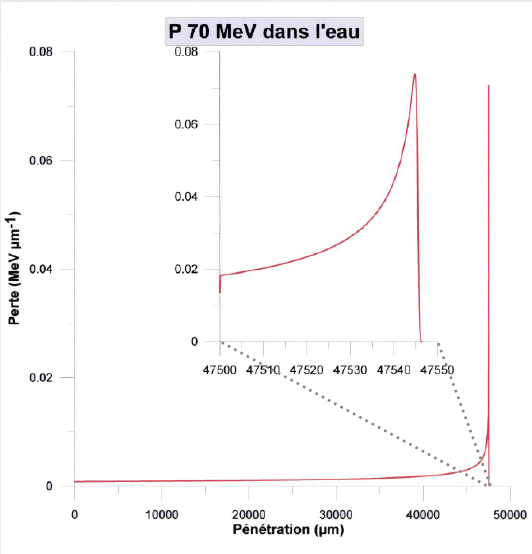
\includegraphics[width=0.5\textwidth]{Images1/picbragg.PNG}
    \caption{Courbe de Bragg théorique pour des protons de 70 \si{MeV} dans l'eau}
    \label{fig:pic_bragg}
\end{figure}

\begin{figure}[H]
    \centering
    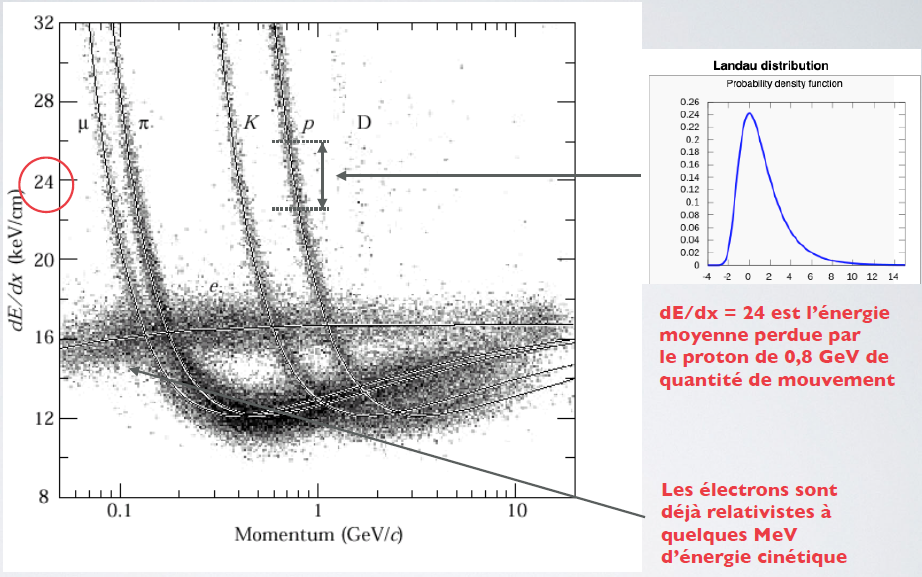
\includegraphics[width=0.66\textwidth]{Images1/perteionisation.PNG}
    \caption{Perte d'énergie par ionisation}
    \label{fig:pertes_ionisation}
\end{figure}

\subsubsection{Perte d'énergie par radiation}
À très haute énergie, les pertes d'énergie par collision deviennent négligeables par rapport aux pertes par radiation. Cet effet n'est important que pour les particules légères.

\begin{figure}[ht]
    \centering
    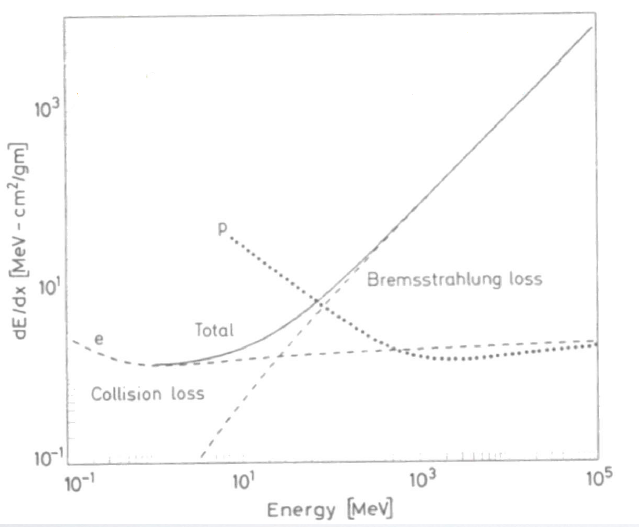
\includegraphics[scale=0.40]{Images1/bremstrucmachin.png}
    \caption{Pertes par collision et par radiation pour des électrons dans du cuivre}
    \label{fig:pertes_collision}
\end{figure}

La courbe qui monte linéairement (attention : graphe logarithmique) en pointillés est le Bremsstrahlung, le rayonnement de freinage qui correspond à l'interaction avec les noyaux n'ayant lieu qu'à hautes énergies, ce qui correspond également au domaine de valeur où la perte par ionisation ou collision (avec les e- des particules cibles) est négligeable. La courbe de cette interaction représentée en pointillés également et est plus ou moins plate, mais remonte à gauche, la zone où elle est prépondérante n'est en fait pas représenté sur le schéma. Le graphe montre également le comportement d'un proton qui réagit donc de manière opposée lors de ces interactions.\\
On constate que quand l'électron devient relativiste ($E>>m$), le rayonnement de freinage (Bremsstrahlung) domine rapidement. Les électrons perdent donc leur énergie par collision sur les électrons du milieu (Möller) et par diffusion élastique sur les noyaux (Mott): il y a déviation de leur trajectoire initiale et rayonnement de freinage. Le rayonnement de freinage varie en $Z^2$ de la cible.

\begin{figure}[ht]
    \centering
    \begin{subfigure}{.5\textwidth}
        \raggedright
        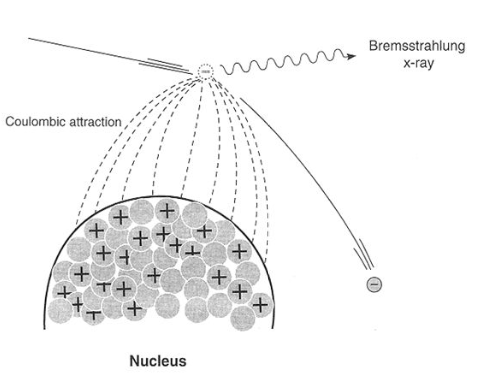
\includegraphics[width=.9\linewidth]{Images1/Bremsstrahlung2.PNG}
        %\caption{A subfigure}
        %\label{fig:sub1}
    \end{subfigure}%
    \begin{subfigure}{.5\textwidth}
        \raggedleft
        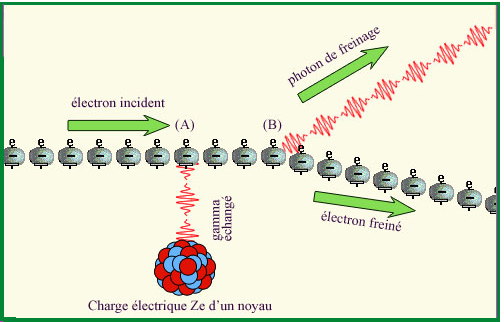
\includegraphics[width=.9\linewidth]{Images1/Bremsstrahlung3.PNG}
        %\caption{A subfigure}
        %\label{fig:sub2}
    \end{subfigure}
    \caption{Mécanisme du rayonnement de freinage}
    \label{fig:rayonnement_freinage}
\end{figure}

\paragraph{Notes supplémentaires sur le Bremsstrahlung:} Le phénomène de rayonnement de freinage (Fig. \ref{fig:rayonnement_freinage}) (Bremsstrahlung en allemand) concerne des particules porteuses d’une charge électrique dont la vitesse est proche de la vitesse de la lumière. Il intervient quand cette particule ultrarelativiste interagit avec un fort champ électrique ou magnétique, qui peut être naturel (le champ électrique d’un noyau) ou produit par l’homme (le champ d’aimants dans un accélérateur de particules). Les électrons et positons qui atteignent facilement des vitesses proches de celle de la lumière du fait de leur très faible masse sont les premiers concernés par le phénomène. \\

Le rayonnement de freinage intervient peu dans le domaine de la radioactivité, les électrons des désintégrations bêta n'étant souvent pas assez énergiques. Par contre, il joue un rôle important dans le rayonnement cosmique et le fonctionnement des accélérateurs de particules. \\

Sous l’effet de l’interaction, l’électron ou le positon, émets un photon qui emporte une partie de son énergie. L’électron est freiné et sa trajectoire modifiée. Le rayonnement de freinage est à l’origine d’une déperdition d’énergie dans de grands accélérateurs de particules comme les collisionneurs où les particules sont soumises à l’action de puissants aimants qui courbent leur trajectoire. Les ingénieurs des accélérateurs doivent compenser en permanence cette déperdition.

\subsubsection{Perte d'énergie des photons}
\begin{figure}[ht]
    \centering
    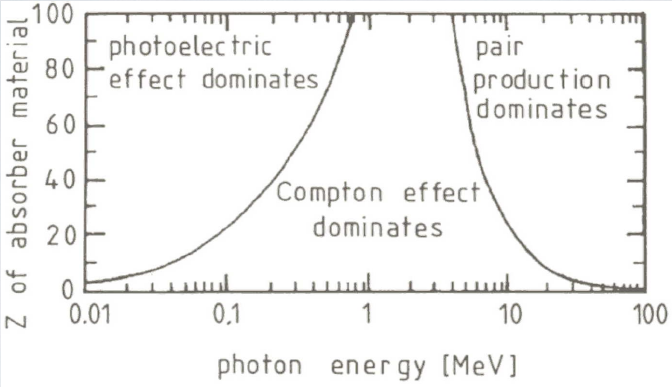
\includegraphics[scale=0.60]{Images1/pertephotons.PNG}
    \caption{Perte d'énergie des photons dans la matière}
    \label{fig:pertes_energie_photos}
\end{figure}
On constate bien sur la figure \ref{fig:pertes_energie_photos} que l'effet Compton est en compétition avec l'effet photoélectrique et la production de paires dans la perte d'énergie par les photons dans la matière\\

La diffusion Compton correspond à la collision d’un photon et d’un électron : le photon rebondit sur un électron cible qui est mis en mouvement et perd de l’énergie. L'électron est arraché à la matière, qui est donc ionisée, et le photon est diffusé. L'effet Compton contribue à l'atténuation des rayons gammas.  Arthur Compton a, en 1923, observé l'allongement de la longueur d'onde du photon dans cette diffusion, effet auquel on a attribué son nom : l'effet Compton.

\begin{figure}[ht]
    \centering
    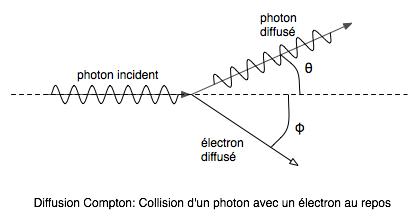
\includegraphics[scale=0.60]{Images1/compton.png}
    \caption{Diffusion Compton}
\end{figure}

La longueur d'onde change selon la formule
\[
    \lambda_f-\lambda_i=\dfrac{h}{m_ec}(1-\cos{\theta})
\]

\subsection{Découverte des rayonnements $\alpha$, $\beta$, $\gamma$}
\subsubsection{Radioactivité}
La radioactivité est le phénomène physique selon lequel des noyaux atomiques instables se transforment spontanément en d'autres atomes (désintégration) en émettant simultanément des particules de matière (électrons, noyaux d'hélium, neutrons, etc.) et de l'énergie (photons et énergie cinétique). Elle a été découverte en 1896 par Henri Becquerel dans le cas de l'uranium, et très vite confirmée par Marie Curie pour le radium. \\

Becquerel étudie le phénomène de phosphorescence. On connaissait déjà ce phénomène via lequel des matériaux émettent de la lumière dans le noir après avoir été exposés à la lumière (éventuellement des rayons X, découverts peu avant). Or, comme expliqué ci-dessus, Becquerel constata le noircissement des émulsions même en l'absence d'exposition à la lumière de sels d'uranium. Il y a donc des substances naturellement radioactives. Serait-ce donc une nouvelle émission similaire aux rayons X ? Quand on met ces substances naturellement radioactives dans une boîte blindée percée d'un petit trou, on observe 3 types de rayonnements: <<positif>>, <<neutre>>, et <<négatif>>, respectivement les rayonnements $\beta$, $\gamma$ et $\alpha$ (Fig. \ref{fig:alpha_beta_gamma}). Ils sont plus ou moins pénétrants dans la matière.

\begin{figure}[ht]
    \centering
    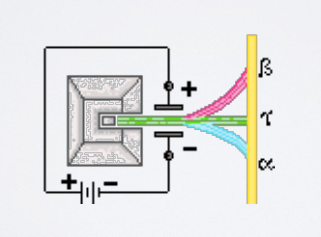
\includegraphics[width=0.4\textwidth]{Images1/rayonnements.PNG}
    \caption{Rayonnements $\alpha$, $\beta$, $\gamma$}
    \label{fig:alpha_beta_gamma}
\end{figure}

\begin{itemize}
    \item \textbf{Rayonnements $\alpha$}: Très vite arrêté par la matière (après une feuille de papier), spectre en énergie sous forme de raies dépendant de l'élément, produits par désintégration $\alpha$. C'est la forme de désintégration radioactive où un noyau atomique X éjecte une particule alpha (forme de rayonnement émis par des noyaux instables de grande masse atomique constitué de deux protons et deux neutrons combinés en une particule identique au noyau d'hélium 4 (hélion)) et se transforme en un noyau Y  de nombre de masse diminué de 4 et de numéro atomique diminué de 2. \\
    Forme générale:
    \[
        ^{A}_{Z}X \longrightarrow ^{A-4}_{Z-2}Y + ^{4}_{2} He ~ (+Q)
    \]
    Exemple:
    \[
        ^{238}U \longrightarrow ^{234}Th + \alpha
    \]
    Bilan énergétique d'une désintégration $\alpha$:
    \[
        Q = T_Y + T_\alpha = [M_{at}(X)-M_{at}(Y)-M_{at}(He)]c^2>0
    \]
    \[
        Q=B(A-4,Z-2)+B(^{4}_{2}He)-B(A,Z)>0
    \]

    \item \textbf{Rayonnements $\beta$}: La radioactivité bêta ou émission bêta est un type de désintégration radioactive dans laquelle une particule bêta (un électron ou un positon) est émise. Aujourd'hui, la désintégration $\beta$ se généralise à toutes les réactions nucléaires impliquant les neutrinos ou antineutrinos. Elle possède un plus grand pouvoir de pénétration (quelques millimètres), et est difficile à observer. Son spectre d'énergie est continu.

    Dans le cas du rayonnement $\beta$, si on trace le graphe de l'énergie des particules (Fig \ref{fig:spectre_beta}), on observe que la conservation de l'énergie n'est pas respectée. C'est ce constat qui inspira l'hypothèse de l'existence du neutrino.

    \begin{figure}[ht]
        \centering
        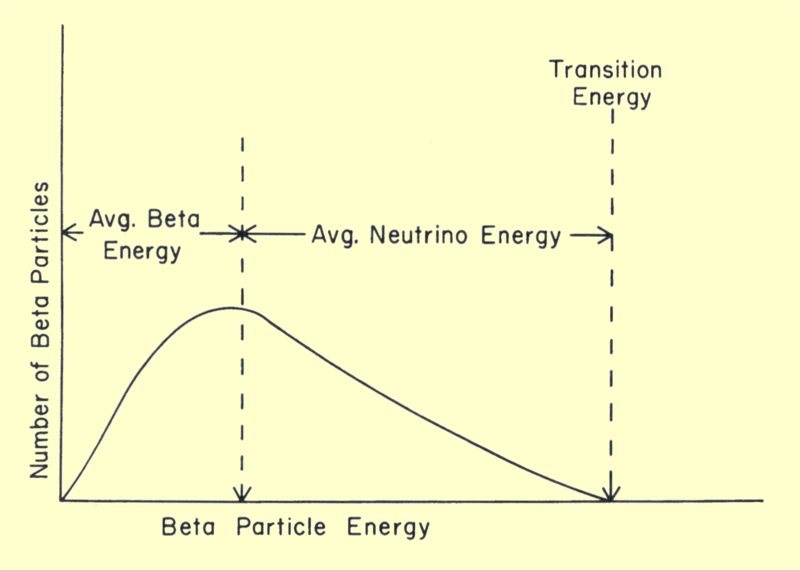
\includegraphics[scale=0.25]{Images1/beta.png}
        \caption{Spectre en énergie de la particule $\beta$}
        \label{fig:spectre_beta}
    \end{figure}

    On parle de désintégration bêta moins ($\beta^{-}$) ou bêta plus ($\beta^{+}$) selon qu'il s'agit de l'émission d'un électron ou d'un positon. Dès lors, on a respectivement les désintégrations suivantes :

    Forme générale:

    \[
        ^{A}_{Z}X \longrightarrow ^{A}_{Z+1}Y + e^- + \bar{\nu}_e
    \]

    \[
        ^{A}_{Z}X \longrightarrow ^{A}_{Z-1}Y + e^+ + \nu_e
    \]

    Exemple:
    \[
        ^{60}_{}Co \longrightarrow ^{60}_{}Ni^{+} + e^- + \bar{\nu}_e
    \]

    \[
        ^{18}_{}F \longrightarrow ^{18}_{}O + e^+ + \nu_e
    \]

    Il peut être intéressant de préciser que l'effet final d'un rayonnement Beta, pour un noyau radioactif instable, est de stabiliser le noyau (rétablir une balance n/p) en convertissant un neutron en proton et inversement (donc en émettant un e$^+$ ou e$^-$).

    \item \textbf{Rayonnements $\gamma$:} Possèdent un pouvoir de pénétration supérieur aux rayonnements alpha et beta et rayons X (ils passent quelques centimètres de plombs), spectre énergétique sous forme de raies. Le mécanisme de production des rayons $\gamma$ est illustré à la figure \ref{fig:rayons_gamma}.
\end{itemize}
\begin{figure}[ht]
    \centering
    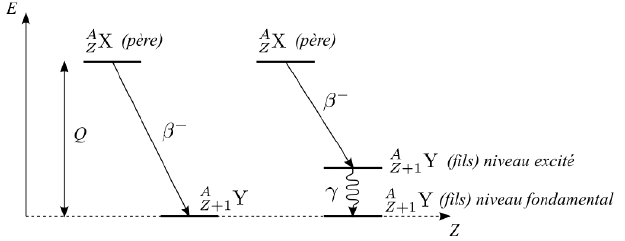
\includegraphics[width=0.8\textwidth]{Images1/gamma.PNG}
    \caption{Rayonnement $\gamma$}
    \label{fig:rayons_gamma}
\end{figure}
Les différents rayonnements obéissent à la loi de désintégration. Leur absorption est également exponentielle:
\[
    I(d)=I_0e^{-\mu d}
\]
où $\mu$ est un coefficient d'absorption\footnote{Ouais il a juste repris de Wikipédia. C'est quand ils passent dans la matière, ils sont absorbés de manière exponentielle et le mu dépend du matériau.}.


\section{Structure du noyau}
\subsection{Concept de section efficace}\label{sec:section_efficace}
\subsubsection{Définition}
Le concept de section efficace (Fig. \ref{fig:section_efficace}) couramment utilisé en physique nucléaire. C'est une grandeur physique reliée à la probabilité d'interaction d'une particule pour une réaction donnée. Son unité est le barn ($1b=10^{-24}cm^2$).
Quand on envoie un faisceau de particules, qu'on assimile à des sphères dures sur une cible, la probabilité d'interaction avec celle-ci est
\[
    \delta P_{int}=\dfrac{\text{Surface des sphères projetées}}{\text{Surface totale}}=\delta N \dfrac{\pi r^2}{S}=n \dif x \pi r^2
\]
où
\begin{itemize}
    \item $\delta N$ est le nombre de boules vues pour une surface S
    \item n est la densité volumique de sphères
    \item $\dif x$ est l'épaisseur de la cible
    \item $\sigma=\pi r^2$ est la section efficace géométrique
\end{itemize}

\begin{figure}[ht]
    \centering
    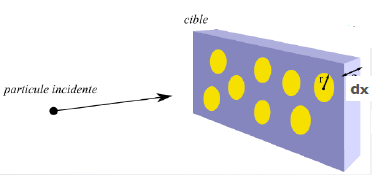
\includegraphics[scale=0.75]{Images1/section_efficace.PNG}
    \caption{Concept de section efficace}
    \label{fig:section_efficace}
\end{figure}
Si on a $N_i$ particules incidentes et $\dif N$ interactions pour une cible d'épaisseur $\dif x$, on admet comme définition de $\sigma$
\[
    \dif N=-N_in\sigma \dif x
\]
La section efficace ne dépend que du projectile et de la cible élémentaire. Pour une section efficace géométrique de l'ordre de \SI{100}{mb}, on a $r_o=\sqrt{\dfrac{\sigma}{\pi}}\sim \SI{e-15}{m} = \SI{1}{fm}$, ce qui est la taille typique des nucléons. Cela explique que, $\sigma(p+\text{noyau})\propto A^{2/3}$ car rayon du noyau $\propto A^{1/3}$.

\subsubsection{Section efficace d'interaction et temps de vie}
On considère une cible de surface S sur laquelle sont projetées des particules pendant une expérience. La section efficace pour cette réaction est $\sigma$. Si $n_0$ est le nombre de noyaux cibles par \si{cm^3}, alors le nombre total de noyaux cibles est $n_0 V$ = $n_0 S x$ et la section efficace de toutes les cibles est $\sigma_{tot}$ = $\sigma n_0 S X$. On peut donc déduire la probabilité qu'il y ait une réaction:
\[
    P=\dfrac{\sigma_{tot}}{S}
\]
et, sachant que $I$ est le nombre de particules incidentes durant toute l'expérience, le nombre de réactions durant l'expérience
\[
    N=I \sigma n_0 x
\]
Définissons maintenant la section efficace en tenant compte des composantes angulaires lors de la diffusion de la particule (Fig. \ref{fig:diffusion_particule}).

\begin{figure}[ht]
    \centering
    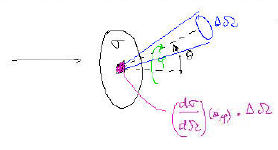
\includegraphics[scale=0.95]{Images1/secdiff.PNG}
    \caption{Représentation de la diffusion d'une particule}
    \label{fig:diffusion_particule}
\end{figure}
\noindent La section efficace telle que la particule part dans l'angle solide $\Delta\Omega$ centré sur $\theta$, $\phi$ est
\[
    \sigma=\int_{4\pi}^{}\fdif{\sigma}{\Omega}\dif \Omega
\]
où $\fdif{\sigma}{\Omega}$ est la section efficace différentielle. On a donc pour le nombre de réactions durant l'expérience
\[
    \dif N=I~n_0~X~\Big(\fdif{\sigma}{\Omega}\Big)~\Delta\Omega \quad\text{avec}\quad \fdif{\sigma}{\Omega}=\dfrac{\dif\sigma}{\dif\phi \dif \;(\cos{\theta})}=\dfrac{1}{2\pi}\fdif{\sigma}{\;(\cos{\theta})}
\]
Pour se représenter la situation, le détecteur correspond à un anneau réalisant toute une révolution autour de l'axe de l'expérience avec un avec $\phi$ (la direction de propagation des particules incidentes) et cela à un certain angle $\theta$.

\subsubsection{Longueur d'atténuation}
On a $\dif N=I_0 n_0 \sigma \dif x=-\dif I$. Si on intègre, on obtient
\[
    \int_{I_{0}}^{I(x)}\dfrac{\dif I}{I}=-\int_0^x n_0.\sigma \dif x
\]
c'est-à-dire que
\[
    I(x)=I_0e^{-n_0.\sigma.x}=I_0.e^{-x/x_0}
\]
On définit $x_0=\dfrac{1}{n_0\sigma}$ comme la longueur d'atténuation.

\subsubsection{Section efficace différentielle}
La section efficace (et donc la probabilité d'interaction) dépend de paramètres géométriques tels que le flux de particules uniforme dans le plan perpendiculaire à la direction de propagation $\Phi=\dfrac{\dif^2N}{\dif t\dif s}$, le nombre de particules diffusées par unité de temps et par unité d'angle solide dans la direction $(\theta, \theta+\dif \theta)$.
\begin{figure}[ht]
    \centering
    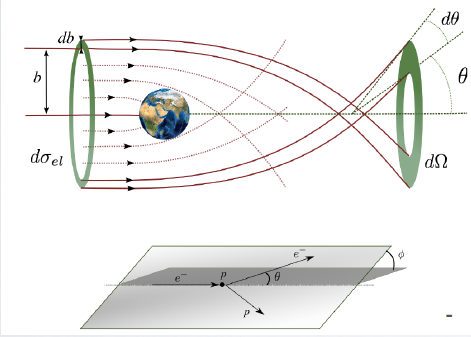
\includegraphics[scale=0.75]{Images1/section_efficace_diff.PNG}
    \caption{Concept de section efficace différentielle}
    \label{fig:section_efficace_diff}
\end{figure}
On a
\[
    \dfrac{\dif^2N}{\dif t\dif \Omega}=\dfrac{\dif^2N}{\dif t\dif \sigma_{el}} \fdif{\sigma_{el}}{\Omega}
\]
Si on mesure le nombre d'électrons à $\theta$ fixé,
\[
    \fdif{\sigma_{el}}{\Omega}=\dfrac{2\pi~b~\dif b}{2\pi \sin{\theta}\dif \theta}
\]
et à angle solide fixé,
\[
    \dif N=N_i~n~\dif x~\dif \Omega~\fdif{\sigma}{\Omega}
\]

\begin{figure}[ht]
    \centering
    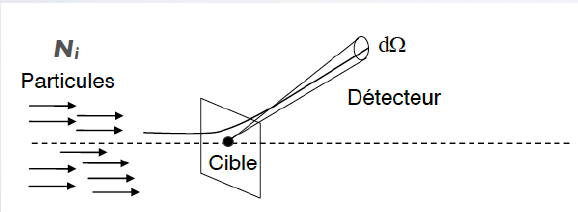
\includegraphics[scale=0.75]{Images1/anglesolide.PNG}
    \caption{Angle solide fixé}
\end{figure}
Remarquons que
\[
    \int(\fdif{\sigma}{\Omega})\dif \Omega=\sigma_{tot}
\]
Du fait de la symétrie, toutes les particules qui ont des paramètres d'impact compris entre $b$ et $b+\dif b$ seront diffusées entre $\theta$ et $\theta+\dif\theta$. Elles sont donc associées à une <<surface>> $2\pi b\cdot \dif b$ perpendiculaire au faisceau (figure \ref{fig:surface_de_diffusion}).
\begin{figure}[ht]
    \centering
    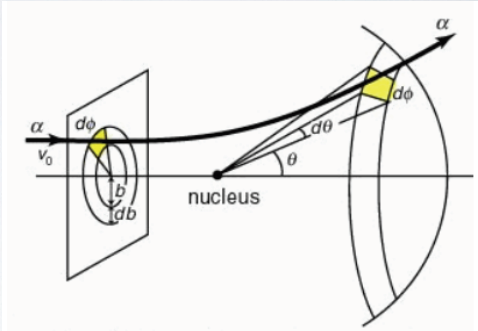
\includegraphics[scale=0.75]{Images1/surface_perp.PNG}
    \caption{<<Surface de diffusion>>}
    \label{fig:surface_de_diffusion}
\end{figure}
Pour une épaisseur x
\[
    \dif N=N_i~n_{\text{cible}}~x~\left(\fdif{\sigma}{\Omega}\right)\dif \Omega
\]
Si on intègre sur l'angle phi, on obtient la définition de \textbf{section efficace différentielle}
\[
    \fdif{\sigma}{\Omega}=\dfrac{2\pi b \dif b}{\dif \Omega}=\dfrac{2\pi~b~\dif b}{2\pi \sin{\theta}\dif\theta}=\dfrac{b}{\sin{\theta}}\abs{\fdif{b}{\theta}}
\]

\subsubsection{Section efficace de Rutherford}
Le développement est très bien expliqué sur \url{http://res-nlp.univ-lemans.fr/NLP_C_M13_G01/co/Contenu17.html}. L'auteur ne fait pas tout à fait comme Lemaître, mais arrive au même résultat.

\subsubsection{Expérience de Geiger et Marsden}
Cette expérience montra que la partie chargée positivement de la matière est concentrée en un espace de petit volume, le noyau atomique. L'expérience est réalisée sous vide. De la matière radioactive émettant des particules $\alpha$ est placée dans une boîte et le faisceau de particules $\alpha$ est orienté en direction d'une très fine feuille d'or (6 000 $\angstrom$). Derrière cette couche d'or, un écran est placé ; il est enrichi d'une substance chimique permettant de visualiser, par un scintillement lumineux, la collision par les particules $\alpha$ (Fig. \ref{fig:geiger_marsden}).

\begin{figure}[ht]
    \centering
    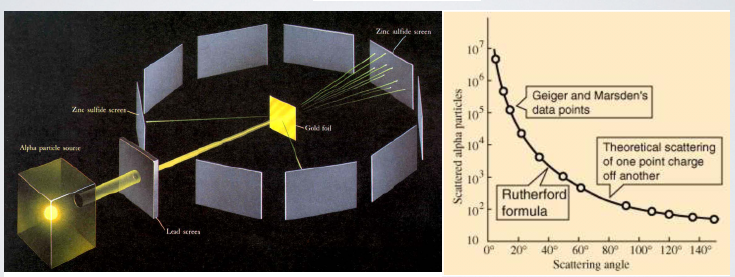
\includegraphics[scale=0.75]{Images1/geiger.PNG}
    \caption{Expérience de Geiger et Marsden : Dispositif - Comparaison prédictions/mesures}
    \label{fig:geiger_marsden}
\end{figure}

Plusieurs minutes après la disposition du matériel, différents points lumineux apparaissent sur l'écran et ces points ne sont pas tous dans l'orientation du faisceau, mais certains étalés sur de grands angles. Rutherford eut ainsi la surprise d'observer une sorte de rebond des particules alpha.

La rétrodiffusion de particules $\alpha$ ne peut s’expliquer que par des chocs élastiques entre les particules alpha et des noyaux atomiques beaucoup plus massifs! Le modèle atomique du flan aux raisins ne résiste évidemment pas à ces observations qui mèneront au modèle de Rutherford (Fig. \ref{fig:mod_rutherford}).
\begin{figure}[ht]
    \centering
    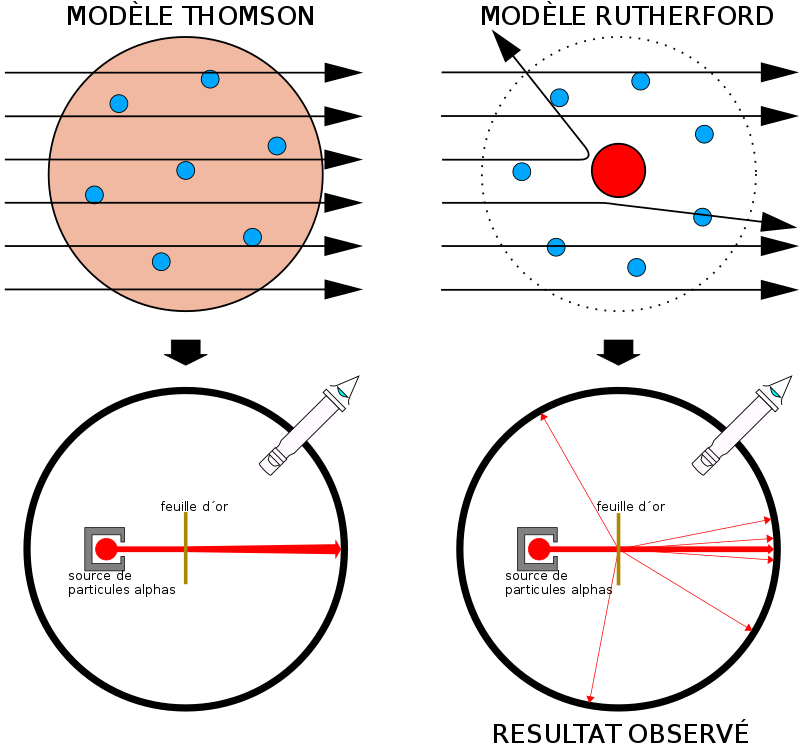
\includegraphics[scale=0.25]{Images1/thom_ruth.png}
    \caption{Modèle de Thomson VS modèle de Rutherford}
    \label{fig:mod_rutherford}
\end{figure}
La distance d'approche minimale calculée par Rutherford satisfait à l'équation

$$\dfrac{1}{2}mv_0^2=\dfrac{1}{4\pi\epsilon_0}\dfrac{Zze^2}{r_\text{min}}$$

Si on projette des $\alpha$ de plus haute énergie sur du plomb par exemple, on observe une diminution du nombre de particules rétrodiffusées à cause de l'interaction forte à courte distance. En effet, les $\alpha$ sont alors absorbés par les noyaux.

\subsection{Découverte du proton}
En 1914, on veut élaborer une théorie du noyau. De quels éléments dispose-t-on ? Le numéro atomique Z, la masse atomique A, le fait qu'un même élément chimique puisse exister sous forme de plusieurs isotopes avec A différents, la radioactivité alpha (il y a des particules alpha, qui sont des noyaux d'hélium, dans certains noyaux), la radioactivité beta (il y a des particules beta, qui sont des électrons, dans certains noyaux). \\
En 1911, Rutherford part des 2 observations que pour la plupart des noyaux, $A \sim 2Z$ et que certains noyaux émettent des particules alpha. Il suggère donc que tous les noyaux, hormis l'hydrogène, sont des assemblages de particules alpha. \\
Cependant, beaucoup d'arguments s'opposent à cette théorie: la moitié des charges électriques Z sont impaires, les masses de la plupart des éléments lourds sont supérieures au double de leur charge électrique, et l'écart s'accroit avec la masse (exemple: du Fer A=56, Z=26 au Plomb A=207, Z=82).  Cela suggère un modèle mixte: hélium + autre chose ? Alors, pourquoi ne pas former directement les noyaux par des assemblages de noyaux d'hydrogène, puisque la plupart des masses atomiques sont des multiples entiers de la masse de l'hydrogène ? Il existe une objection majeure à cette proposition : si on forme le noyau de masse A avec A noyaux d'hydrogène, ce noyau a une charge électrique +Ae, et non +Ze... Rutherford suppose alors à l'époque que le noyau possède en plus A-Z électrons, ce qui expliquerait en plus que les noyaux perdent des électrons dans la radioactivité beta. Cette théorie du noyau avait 2 conséquences:

\begin{itemize}
    \item Il y a des noyaux d'hydrogène dans TOUS les noyaux
    \item Il doit exister un mécanisme séparant les Z électrons dits périphériques des A-Z électrons nucléaires.
\end{itemize}

Le premier point a des conséquences expérimentales un peu étranges que Rutherford mit en avant: en 1915, avec Marsden il bombarde de l'hydrogène avec des particules alpha (source = radon), à l'aide du dispositif illustré ci-dessous. La chambre est remplie de gaz, une source d’alphas (la plaque sur le pied) les projette sur les noyaux du gaz (Fig. \ref{fig:chambre_bombardement_H}). Les alphas, les noyaux du gaz et les protons provoquent des scintillations différentes sur l’écran de sulfure de zinc à droite, observé au microscope. Ils observent des reculs de l'hydrogène, caractérisés par des traces plus fines que celles des alphas.

\begin{figure}[ht]
    \centering
    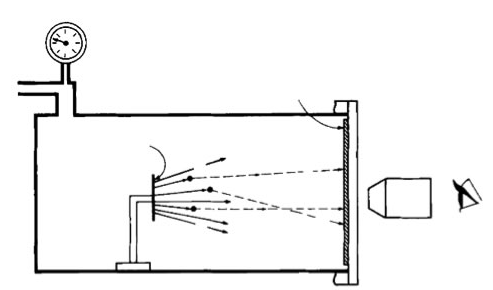
\includegraphics[scale=0.75]{Images1/bombardement.PNG}
    \caption{Chambre de bombardement d'hydrogène}
    \label{fig:chambre_bombardement_H}
\end{figure}

Marsden remarqua une émission d'hydrogène par le radon avant le remplissage de la chambre en hydrogène. Rutherford ne crut pas à une nouvelle forme de radioactivité, mais plutôt à une contamination de l'appareillage par l'hydrogène. Il nota plus tard que s'il remplissait la chambre d'oxygène ou de gaz carbonique, le nombre de scintillations attribuables à l'hydrogène diminuait, comme il s'y attendait, mais ce nombre augmentait quand la chambre était remplie d'air et plus encore quand elle était remplie d'azote ! Ce phénomène de <<fuite d'hydrogène>> n'apparaissait que pour des alphas d'énergie supérieure à 1.21 \si{MeV}. Rutherford supposa donc une ionisation des molécules d'eau présentes dans l'air ou l'azote. Mais après suppression de l'eau, le phénomène persistait, Rutherford en conclut donc que l'azote se transmutait au cours de la collision avec les alphas, et que les noyaux d'hydrogène appartenaient au noyau d'azote. Rutherford pensait observer la réaction
\begin{center}
    alpha + azote $\longrightarrow$ hydrogène + carbone + alpha
\end{center}
et son interprétation fut la suivante en 1919 :

\begin{itemize}
    \item Carbone: masse atomique 12 = 3 alphas
    \item Oxygène: masse atomique 16 = 4 alphas
    \item Azote: masse atomique 14 = 3 alphas + 2 hydrogènes périphériques, facilement arrachables par l’alpha servant de projectile, dès qu’il avait une énergie suffisante (les 1.21 \si{MeV} requis)
\end{itemize}

Cette interprétation a 2 conséquences majeures: les transmutations nucléaires ne sont pas limitées aux éléments lourds (radioactifs) et les collisions d'alphas permettent de sonder en profondeur les noyaux, pas seulement leur cortège d'électrons.

Rutherford a ainsi développé une nouvelle technique de recherche, malheureusement limitée par la faible énergie des alphas. S'en suivit pour remédier à ce problème la conception d'accélérateurs, comme le premier cyclotron, par Lawrence (Fig. \ref{fig:lawrence_cyclo}).

L’utilisation de la chambre de Wilson (ou chambre à brouillard) (Fig. \ref{fig:chambre_wilson}) se révéla bien plus pratique que les écrans au sulfure de zinc, car elle permettait de visualiser, et d’enregistrer, le résultat des collisions sous la forme de traces des particules avant et après collision, et même parfois de mesurer leur charge et leur énergie. En 1920, Chadwick mesura la charge des noyaux Cu, Ag, Pt par diffusion alphas. Ayant démontré qu’il y avait bien des noyaux d’hydrogène dans le noyau d’azote, Rutherford les baptisa proton en 1920.

\begin{figure}[ht]
    \centering
    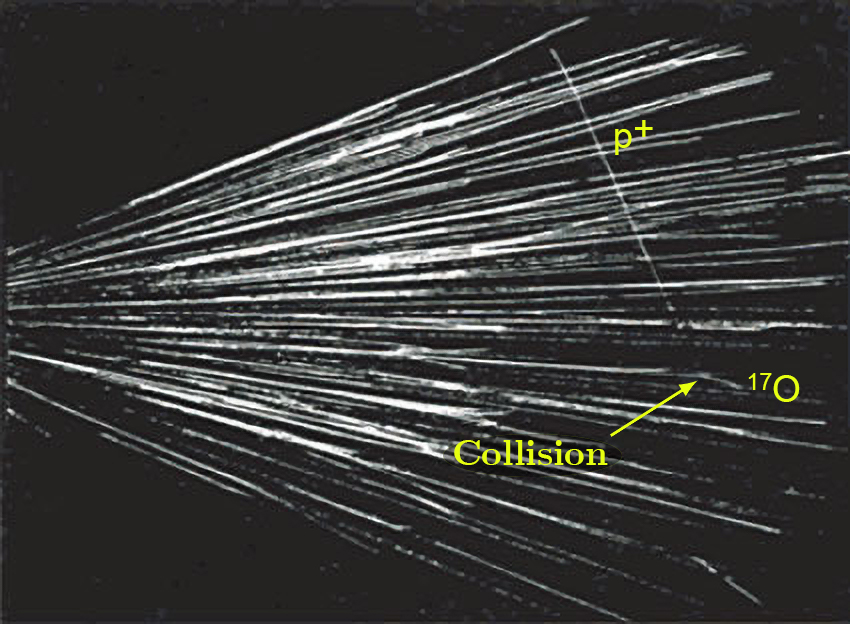
\includegraphics[width=0.7\textwidth]{Images1/collisions_alpha_proton.jpg}
    \caption{La chambre à brouillard de Wilson: des particules alpha provenant d'une source sur la gauche laissent une traînée des gouttelettes dans une chambre à brouillard remplie d'azote. L'une d'entre elles frappe un noyau d'azote à droite, donnant un proton partant vers le haut gauche et un noyau d'oxygène partant vers le bas à droite. (Blackett 1935)}
    \label{fig:chambre_wilson}
\end{figure}

Les expériences de Rutherford validaient --- apparemment --- l’image du noyau comme un assemblage de A protons avec A-Z électrons <<nucléaires>>, associés pensait-il en sous-structures alpha. De nombreux modèles qualitatifs furent élaborés pour rendre compte des régularités empiriques, mais ils étaient peu prédictifs, et surtout ils entrèrent très vite en conflit avec la nouvelle mécanique quantique (Fig. \ref{fig:to_be_continued})...

\begin{figure}[ht]
    \centering
    \begin{minipage}{.5\textwidth}
        \centering
        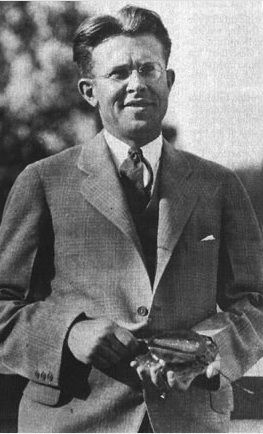
\includegraphics[height=5.5cm]{Images1/cyclo.PNG}
        \captionof{figure}{Lawrence et un bébé cyclotron}
        \label{fig:lawrence_cyclo}
    \end{minipage}%
    \begin{minipage}{.5\textwidth}
        \centering
        
\includegraphics[height=5.5cm]{Images1/mama.png}
        \captionof{figure}{To be continued...}
        \label{fig:to_be_continued}
    \end{minipage}
\end{figure}

\subsection{Découverte du neutron}
En gros:
\begin{itemize}
    \item 1931: Joliot et sa femme Curie bombardent du Béryllium avec une source d'alpha et observent une radiation très pénétrante (Fig. \ref{fig:joliot_curie}).

    \begin{figure}[H]
        \centering
        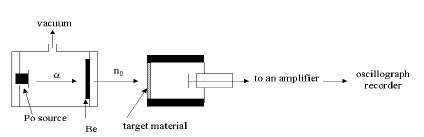
\includegraphics[scale=0.99]{Images1/joliotcurie.PNG}
        \caption{Expérience de Joliot-Curie}
        \label{fig:joliot_curie}
    \end{figure}

    Hypothèse de Bothe et Becker: ce sont des rayons X. Hypothèse de Joliot et Curie: ce sont des rayons gamma, et la réaction est donc similaire à celle de l'effet Compton sur des protons. Ils pensent cela, car ils observent l'émission de protons éjectés d'une cible de paraffine bombardée avec cette radiation. (protons mesurés avec une chambre à ionisation.) Hypothèse de Chadwick: la radiation correspond à une interaction avec une nouvelle particule neutre donc la masse est similaire à celle du proton selon la réaction
    \[
        ^{4}_{2}He + ^{9}_{4}Be \rightarrow ^{12}_{6}C + ^{1}_{0}n
    \]

    \item Il mesure que les protons éjectés ont des vitesses maximales $v=\dfrac{c}{10}$ dans une chambre à brouillard, compatible avec des photons de \SI{50}{MeV} incidents, ce qui est très élevé pour des rayons gamma qui ont normalement une énergie de quelques \si{MeV}.

    \item Il note le recul de noyaux d'azote si l'azote est introduit dans la chambre à brouillard (Fig \ref{fig:recul_azote}) ! Ici aussi, le parcours de l'azote dans le chambre est tel que l'énergie est bien plus élevée que 400 \si{keV} (qui serait l'énergie maximale si on avait des photons de \SI{50}{MeV})


    \begin{figure}[ht]
        \centering
        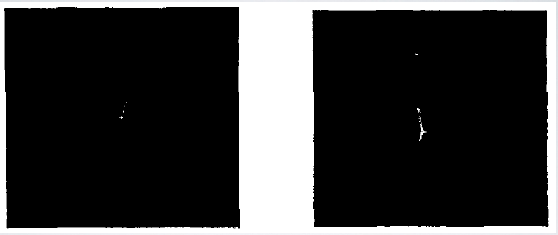
\includegraphics[scale=0.85]{Images1/reculazote.PNG}
        \caption{Gauche: Recul de ce qui pourrait être un ion d'azote - Droite: Recul d'un ion d'azote qui fait interaction élastique avec un autre noyau d'azote}
        \label{fig:recul_azote}
    \end{figure}

    \item Il observe aussi d'autres réactions inélastiques type $n + ^{14}N \rightarrow ^{11}B + \alpha $ (voir figure \ref{fig:coll_inelastique})

    \begin{figure}[ht]
        \centering
        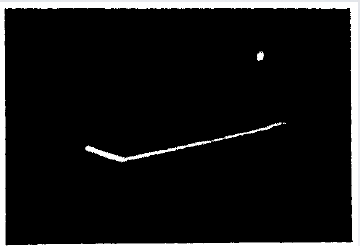
\includegraphics[scale=0.80]{Images1/inelastique.PNG}
        \caption{Réactions inélastiques entre un neutron et l'azote de la chambre}
        \label{fig:coll_inelastique}
    \end{figure}
\end{itemize}
Comment a-t-on déterminé la masse de la nouvelle particule, le neutron ? Pour la collision
\[
    m + M \rightarrow m + M
\]
où m a une vitesse initiale v et M est au repos, on a que la vitesse maximale de M après la collision est
\[
    \dfrac{2mv}{(m+M)}
\]
Sachant que les vitesses maximales pour le proton de recul et l'azote sont respectivement \SI{3.7e9}{cm/s} et \SI{1.7e8}{cm/s}, on obtient $m$ = $90\%~M_\text{proton}$. En bons physiciens, on considère donc que $M_\text{proton}$ = $M_{neutron}$. (En vrai, des mesures plus précises ont indiqué que la différence entre le deux vaut 0,14 pour cent de la masse moyenne du proton et du neutron.)

\subsection{Mesure de la masse des noyaux et énergie de liaison}
Expérimentalement, on détermine la masse des noyaux via la technique de spectrographie de masse (Fig. \ref{fig:spectro_masse}). Elle consiste à identifier les masses des composants d'un échantillon de manière individuelle grâce à un faisceau d'ions. Une source produit ce faisceau possédant une certaine distribution de vitesses. Un sélecteur de vitesses permet seulement aux ions ayant une vitesse particulière de passer (le reste du faisceau est défléchi), et la sélection de moments grâce à un champ magnétique permet l'identification des masses individuelles.
\begin{figure}[ht]
    \centering
    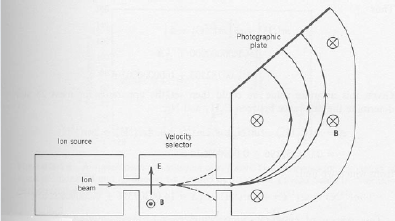
\includegraphics[scale=0.80]{Images1/spectro.PNG}
    \caption{Principe du spectrographe de masse}
    \label{fig:spectro_masse}
\end{figure}
Soit un atome avec A nucléons, Z protons et Z électrons. Sa masse M(A,Z) s'écrit
\[
    M(A,Z) = m(A,Z) + Z \cdot m_e - E^{\text{atome}}_{\text{liaison}}
\]
avec m(A,Z) la masse du noyau de l'atome, définie par
\[
m(A,Z)=Z.m_p+(A-Z)m_n-E^{\text{nucléaire}}_{\text{liaison}}
\]
Définissons l'énergie de liaison de l'atome par
\[
    B=E^\text{atome}_\text{liaison}+E^{\text{noyau}}_{\text{liaison}}
\]
Elle est largement dominée par l'énergie de liaison nucléaire de sorte que dans la suite, on approximera B comme l'énergie de liaison du noyau. Cette énergie de liaison est généralement négligeable devant l'énergie de masse.
En guise d'exemple, on considère le système de 2 nucléons (le deutérium). Évaluons l'énergie de liaison de son noyau, le deuton. On a
\[
    M(^{2}_{}D)=2.014~u
\]
où \[u=\dfrac{1}{12}M(^{12}_{}C)=931.495 \cdot \dfrac{\si{MeV}}{c^2}=\SI{1.66054e-27}{kg}\]
Connaissant les masses du proton, neutron et électron, on trouve que
\[
    B(^{2}_{}D) = \SI{2.227}{MeV}/c^2
\]
soit $0.12\%~M(^{2}_{}D)$.

\subsection{Découverte des rayons cosmiques et de l'antimatière}
Le rayonnement cosmique est le flux de noyaux atomiques et de particules de haute énergie (relativistes) qui circulent dans le milieu interstellaire. La source de ce rayonnement se situe selon les cas dans le Soleil, à l'intérieur ou à l'extérieur de notre galaxie. Certaines astroparticules qui composent le rayonnement cosmique ont une énergie qui dépasse 1020 eV et qui n'est expliquée par aucun processus physique identifié. Le rayonnement cosmique est principalement constitué de particules chargées : protons, noyaux d'hélium, antiprotons, électrons, positrons et particules neutres (rayons gamma, neutrinos et neutrons).\\[0,2cm]
La découverte du rayonnement cosmique a lieu au début du XXe siècle avec les observations de Victor Hess effectuées en 1912 depuis un ballon. Il observe une légère diminution du taux de décharge de l'électroscope entre 0 et 500m d'altitude (mesure effectuée initialement entre la base de la tour Eiffel et son sommet, à 324m d'altitude).

\begin{figure}[ht]
    \centering
    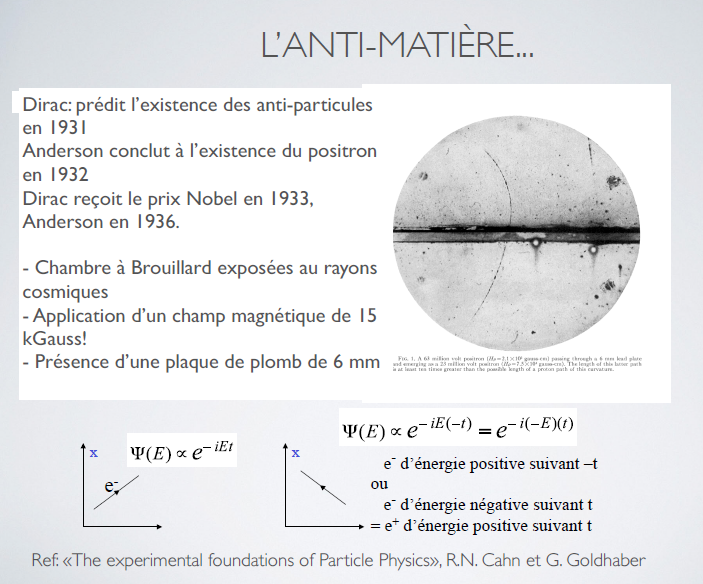
\includegraphics[scale=0.80]{Images1/antimatiere.PNG}
    \caption{Découverte de l'antimatière}
\end{figure}
\newpage


\newpage
\part{Physique atomique (Xavier Urbain et Mariko Terao)}
\begin{center}
    En cas de questions ou de remarques sur cette partie : contactez Eléonore Lieffrig, Justin Gérard %ou Valentin Fonck.
\end{center}
Concernant cette partie, 2 syllabus écrits par Prof. Mariko Terao sont disponibles sur Moodle. Il reste donc les slides de Xavier Urbain à traiter.

\section{Rappels sur l'atome d'hydrogène}

\subsection{Mise en contexte du problème}

Considérons l'atome d'hydrogène où $M$ et $m$ sont respectivement la masse du noyau et la masse de l'électron. Soit $\Psi$ la fonction d'onde du système. L'évolution de cette dernière est bien entendu décrite par l'équation de Schrödinger:

\[\imag\hbar \dfrac{\partial}{\partial t}\Psi=H\Psi\]

où \begin{align}
H&\eq T+V \\
&\eq -\dfrac{\hbar^2}{2\mu}\nabla^2-\dfrac{Ze^2}{4\pi \epsilon_0 r}
\end{align}
avec $\mu=\dfrac{Mm}{(m+M)}$ la masse réduite du système et $r$ la distance entre le noyau et l'électron. Le potentiel $V$ étant dans ce cas indépendant du temps, on peut montrer que les solutions de l'équation de Schrödinger sont de la forme

\[
    \Psi(\Vec{r},t) \eq \Psi_E(\Vec{r}) \cdot \exp(-\dfrac{\imag}{\hbar}Et)
\]


On va chercher les états stationnaires tels que $H\Psi_E=E\Psi_E$ (équation de Schrödinger indépendante du temps), $\Psi_E(\Vec{r})$ étant la fonction d'onde au temps $t=0$. Pour cela, réécrivons la contribution cinétique à l'hamiltonien en coordonnées sphériques. Cela nous permettra de séparer notre équation en une partie radiale et une partie angulaire où apparaîtra l'opérateur moment angulaire $L^2$. Ce dernier sera qualifié de terme "centrifuge" en référence à l'effet de rotation du système, qui est la propriété de $L^2$.

\subsection{Passage aux coordonnées sphériques}

En coordonnées sphériques,

\begin{align*}
    T&\eq
    \dfrac{-\hbar^2}{2\mu}\left[\dfrac{1}{r^2}\dfrac{\partial}{\partial r}\left(r^2\dfrac{\partial}{\partial r}\right)+\dfrac{1}{r^2\sin{\theta}}\dfrac{\partial}{\partial \theta}\left(\sin{\theta}\dfrac{\partial}{\partial \theta}\right)+\dfrac{1}{r^2(\sin{\theta})^2}\dfrac{\partial ^2}{\partial\phi^2}\right]\\
    &\eq-\dfrac{\hbar^2}{2\mu}\left[\dfrac{1}{r^2}\dfrac{\partial}{\partial r}\left(r^2\dfrac{\partial}{\partial r}\right)-\dfrac{\Vec{L}^2}{\hbar^2r^2}\right]
\end{align*}
Les opérateurs $H$, $L_z$ et$\Vec{L}^2$ commutent entre eux. Cela signifie qu'ils possèdent un ensemble commun de fonctions propres. Or, on sait que les fonctions propres des opérateurs $\Vec{L}^2$ et $L_z$ sont les harmoniques sphériques

\begin{align*}
    Y_{lm}(\theta, \phi) \eq (-1)^m \left[ \dfrac{(2l+1)(l-m)!}{4\pi(l+m)!}\right]^{1/2} \cdot P^{l}_{m}(\cos{\theta})e^{im\phi} \qquad m\ge0
\end{align*}
Rappelons donc quelques identités impliquant les harmoniques sphériques:


\[
    Y_{l}^{-m}(\theta, \phi)\eq (-1)^m\left[Y_{l}^{m}(\theta, \phi)\right]^{*}
\]

\[
    L^2Y_{lm}\eq-\hbar^2 \left[\dfrac{1}{\sin{\theta}}\dfrac{\partial}{\partial\theta}\left(\sin{\theta}\dfrac{\partial}{\partial\theta}\right)+\dfrac{1}{\sin{\theta}^2}\dfrac{\partial^2}{\partial\phi^2}\right]Y_{lm}\eq l(l+1)\hbar^2Y_{lm}
\]

\[
    L_zY_{lm}\eq-\imag\hbar\dfrac{\partial}{\partial\phi}Y_{lm}\eq m\hbar Y_{lm}
\]
Les harmoniques sphériques sont donc bien des fonctions propres de $L^2$ (resp. $L_z$) de valeurs propres $l(l+1)\hbar^2$ (resp. $m\hbar$). Etant donné que les opérateurs $H$, $L_z$ et $L^2$ commutent, les harmoniques sphériques sont également fonctions propres de $H$. Ainsi, ces dernières sont forcément de la forme

\[
    \Psi_{Elm}(r,\theta,\phi)\eq R Y_{lm}(\theta,\phi)
\]
où $R$ est un facteur indépendant des coordonnées angulaires. Les fonctions propres de $H$ étant dépendantes de ces coordonnées angulaires mais également de $r$, le facteur $R$ doit donc être fonction de $r$, ce qui donne finalement

\begin{equation}
    \Psi_{Elm}(r,\theta,\phi)\eq R_{Elm}(r) Y_{lm}(\theta,\phi)
    \label{decompopsi}
\end{equation}



\subsection{Constantes du mouvement}
Considérons l'équation de Schrödinger et sa complexe conjuguée:

\[
    \imag \hbar \dfrac{\partial}{\partial t} \Psi \eq H \Psi
\]

\[
    -\imag \hbar \dfrac{\partial}{\partial t} \Psi ^{*}\eq (H \Psi)^{*}
\]
Le taux de variation au cours du temps de la valeur moyenne d'un opérateur $A$ est donc donnée par

\begin{align*}
    \fdif{}{t}  \braket{A} &\eq\fdif{}{t} \int \Psi^{*} A \Psi \dif\vec{r} \\
    &\eq \int\left(\dfrac{\partial\Psi^{*}}{\partial t}A \Psi + \Psi^{*} A \dfrac{\partial \Psi }{\partial t } + \Psi^{*} \dfrac{\partial A}{\partial t}\Psi \right) \dif\vec{r}\\
    &\eq \Big< \dfrac{\partial A}{\partial t} \Big> +\dfrac{1}{\imag \hbar} \int \Psi^{*} (AH-HA)\Psi \dif\vec{r}
\end{align*}
Dans le cas particulier où l'opérateur $A$ est indépendant du temps, on a


\[
  \fdif{}{t}\left<A\right>\eq \dfrac{1}{\imag\hbar}\big<[A,H]\big>
\]
Ainsi, si $A$ commute avec l'hamiltonien $H$, sa valeur moyenne ne varie pas au cours du temps, c'est une constante du mouvement ($\equiv$ grandeur ne variant pas lors de l'évolution du système).


\subsection{Séparation des variables: équation radiale}
Revenons\footnote{pour ceux qui veulent, un développement assez similaire est fait de
manière plus claire dans le chapitre 4 de Quantique 2} à l'équation \eqref{decompopsi}

\[
    \Psi_{Elm}(r, \theta, \phi)\eq R_{El}(r)Y_{lm}(\theta, \phi)
\]
Si on substitue cette décomposition dans l'équation de Schrödinger indépendante du temps $H\Psi_E=E\Psi_E$ avec l'expression de $T$ que l'on avait développée en coordonnées sphériques, on trouve que la fonction radiale $R_{El}$ doit satisfaire à

\begin{equation}
    \left[-\dfrac{\hbar^2}{2\mu}\left[\dfrac{1}{r^2}\fdif{}{r}\left(r^2\fdif{}{r}\right) - \dfrac{l(l+1)}{r^2}\right]+V(r)\right]R_{El}(r)\eq ER_{El}(r)
    \label{44}
\end{equation}
Posons $R_{El}(r)\eq \dfrac{1}{r}u_{El}(r)$. \eqref{44} devient

\[
    \left[-\dfrac{\hbar^2}{2\mu}\ffdif{}{r}+\dfrac{l(l+1)\hbar^2}{2 \mu r^2}+V(r)\right] u_{El}(r)\eq Eu_{El}(r)
\]
$\dfrac{l(l+1)\hbar^2}{2\mu r^2}$ est un terme de répulsion (répulsion centrifuge plus exactement). En r=0, il faut que la fonction d'onde réduite s'annule pour éviter la divergence:

\[u_{El}(0)=0\]
On a

\begin{equation}
    \left[\ffdif{}{r}+\dfrac{2\mu}{\hbar^2}[E-V_\text{eff}(r)]\right]u_{El}(r)\eq 0
    \label{jsp}
\end{equation}
où on a défini le potentiel effectif

\[
    V_\text{eff}(r)\eq -\dfrac{Ze^2}{4\pi \epsilon_0}\dfrac{1}{r}+\dfrac{l(l+1)\hbar^2}{2\mu r^2}
\]
Le premier terme est le potentiel coulombien et le deuxième est le `potentiel' centrifuge. Plus $l$ est grand, plus ce potentiel s'ajoutant au coulombien va être grand près de l'origine, ce qui va pousser la fonction d'onde à plus grande distance. On a un effet similaire sur un carrousel : un point sur un carrousel tournant ressentira une force voulant l'expulser de l'attraction.

la figure \ref{fig:potentieleffectif} représente le potentiel effectif pour différentes valeurs de $l$ (et pour Z=1).

\begin{figure}[htp]
    \centering
    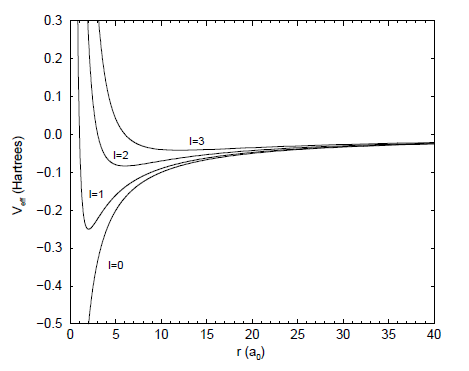
\includegraphics[scale=0.80]{Images2/rad.PNG}
    \caption{Potentiel effectif $V_\text{eff}$ pour Z=1}
    \label{fig:potentieleffectif}
\end{figure}
A courte distance, on observe que le terme en $\dfrac{1}{r^2}$ domine. Sans moment angulaire, on a juste un potentiel coulombien. En ajoutant un terme en $\dfrac{1}{r^2}$ ("potentiel centrifuge", n'existe que quand on a un moment angulaire non nul) on obtient une barrière de potentiel à courte distance. Ainsi, le moment angulaire va empêcher l'électron d'approcher du noyau (c'est-à-dire du proton dans notre cas de l'hydrogène). On s'attend donc, lorsque qu'on va calculer la fonction d'onde radiale, à ce qu'elle soit localisée près du noyau lorsque $l=0$ et de plus en plus loin du noyau au fur et à mesure que $l$ grandit.


Il est possible de faire en sorte que l'équation soit plus simple et en unités réduites. Pour que le comportement colle avec ce qu'on sait déjà, il faut qu'à l'infini la probabilité de présence de l'électron tende exponentiellement vers 0, quelque soit la valeur de $l$ car quand on s'éloigne, on atteint une zone où l'énergie totale est inférieure à l'énergie potentielle donc la probabilité de présence de l'onde dans cette zone doit tendre vers 0. C'est une région qui est classiquement interdite, mais tenant compte des effets tunnels, la fonction d'onde y est présente, mais décroît de façon exponentielle.


Posons, pour simplifier les notations, les quantités sans dimension

\[
    \rho\eq\left(-\dfrac{8\mu E}{\hbar^2}\right)^{1/2}r
\]

\begin{equation}
    \lambda\eq\dfrac{Ze^2}{4\pi\epsilon_0 \hbar}\left(-\dfrac{\mu}{2E}\right)^{1/2}\eq Z\alpha\left(-\dfrac{\mu c^2}{2E}\right)^{1/2}
    \label{lambda}
\end{equation}
où $\alpha=e^2/(4\pi\epsilon_0 \hbar c) \approx 1/137$ est la constante de structure fine. Cela nous permet de réécrire l'équation \eqref{jsp} comme


\begin{equation}
    \left[\ffdif{}{\rho}-\dfrac{l(l+1)}{\rho^2}+\dfrac{\lambda}{\rho}-\dfrac{1}{4}\right]u_{El}(\rho)\eq0
    \label{reduite}
\end{equation}
Lorsque $\rho \rightarrow +\infty$, les termes en $\dfrac{1}{\rho}$ et $\dfrac{1}{\rho^2}$ sont négligeables et alors les 2 solutions de \eqref{reduite} sont de la forme exp$(\pm \rho/2)$. Comme on cherche des solutions bornées, on ne garde que la solution asymptotiquement décroissante et donc on a la condition suivante sur notre solution:

\[
    u_{El}(\rho)\sim e^{-\rho/2} \quad \text{pour} \quad \rho \longrightarrow \infty
\]
Ainsi, la fonction $u_{El}(\rho)$ doit être de la forme

\[
    u_{El}(\rho)\eq e^{-\rho/2}f_{El}(\rho)
\]
avec $f_{El}(\rho)$ satisfaisant l'équation

\begin{equation}
 \left[\fdif{}{\rho^2}-\fdif{}{\rho}-\dfrac{l(l+1)}{\rho^2}+\dfrac{\lambda}{\rho}\right]f_{El}(\rho)\eq0
 \label{fel}
\end{equation}
De plus, quand $\rho \longrightarrow 0$, c'est le terme en $1/\rho^2$ qui devient dominant dans \eqref{reduite}. La solution régulière est de la forme

\[
    u_{El}(\rho) \sim \rho^{l+1} \qquad \text{pour} \qquad \rho \longrightarrow 0
\]
Supposons que $f_{El}(\rho)$ puisse s'écrire sous la forme

\[
    f_{El}(\rho)\eq\rho^{l+1}g_{El}(\rho)
\]
où on développe $g_{El}$ en série:

\[
    g_{El}(\rho)\eq\sum_{k=0}^{\infty} c_k\rho^k \quad c_0 \neq 0
\]
En injectant ce développement de solution dans \eqref{fel}, on obtient l'équation que doit satisfaire $g_{El}(\rho)$:

\begin{equation}
    \left[\rho\ffdif{}{\rho}+(2l+2-\rho)\fdif{}{\rho}+(\lambda-l-1)\right]g_{El}(\rho)\eq0
    \label{gel}
\end{equation}
En y substituant notre développement en série, on obtient la relation de récurrence que doivent satisfaire les coefficients $c_k$:

\begin{equation}
    c_{k+1}\eq\dfrac{k+l+1-\lambda}{(k+1)(k+2l+2)}c_k
\end{equation}
Supposons que $g_{El}(\rho)$ soit un polynôme de degré $n_r$. Comme il doit être fini, il faut que $c_{n_{r}+1}$=0 du coup

\[
    n_r+l+1-\lambda\eq0 \quad \Rightarrow \quad \lambda\eq n_r +l+1
\]
$\lambda$ est donc un nombre entier positif. On l'appelle nombre quantique principal de la solution et on le note $n$. La relation \eqref{lambda} fournit la valeur propre $E_n$ de la solution:

\begin{equation}
    E_n\eq -\dfrac{1}{2n^2}\left(\dfrac{Ze^2}{4\pi\epsilon_0}\right)^2\dfrac{\mu}{\hbar^2}\eq -\dfrac{1}{2}\mu c^2 \dfrac{(Z\alpha)^2}{n^2}
\end{equation}

Le spectre d'énergie de l'atome d'hydrogène (c'est-à-dire les valeurs de l'énergie pour différents $n$) est représenté à la figure \ref{fig:spectreH}.
\begin{figure}[htp]
    \centering
    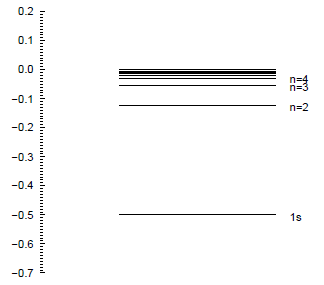
\includegraphics{Images2/spectreH.PNG}
    \caption{Spectre d'énergies de l'atome d'hydrogène. Les énergies sont exprimées en Hartree}
    \label{fig:spectreH}
\end{figure}
Pour chaque nombre quantique principal, on a un certain nombre de sous-niveaux qui est croissant avec $n$ (pour $n=1$ on a le niveau 1s, pour $n=2$ on a 2s et 2p,...). Il y a donc une dégénérescence des niveaux d'énergie qui peuvent donc correspondre à des fonctions d'onde différentes, ce qui va compliquer le spectre. Cette dégénérescence est due (c'est non trivial) à la dépendance en $r^{-1}$ du potentiel coulombien et peut être levée par l'action d'un champ électrique ou magnétique (effets Stark et Zeeman).

Comme la puissance du polynôme $g_{El}$ vaut $n_r=n-l-1$ qui est forcément nul ou positif, il y a $n-1$ valeurs possibles de $l$ pour chaque valeur de $n$: $l=0, 1, ..., n-1$. De plus il y a $2l+1$ valeurs possibles de $m$ pour chaque valeur de $l$: $m=-l, -l+1, ..., l-1, l$. Le degré de dégénérescence du niveau $E_n$ vaut donc

\[
    \sum_{l=0}^{n-1} (2l+1)\eq 2\sum_{l=0}^{n-1} l + n \eq  2 \dfrac{(n-1)n}{2} + n \eq  n^2
\]
On remarque un tassement des niveaux vers la limite d'ionisation (région entre $n=2$ et $n=\infty$).

\subsection{Solution complète}
Il se trouve que les polynômes $g_{El}(\rho)$ sont des polynômes de Laguerre associés. En effet ceux-ci sont définis comme solutions de l'équation différentielle

\begin{equation}
    \left[x\ffdif{}{x}+(K+1-x)\fdif{}{x}+N\right] L_{N}^{K}(x)\eq 0
\end{equation}
L'équation \eqref{gel} est similaire à cette équation, et en les comparant on en déduit même que

\[
    g_{El}(\rho)\eq L_{n-l-1}^{2l+1}(\rho)
\]
En regroupant les résultats des sous-sections précédentes on a donc comme solution pour les fonctions d'onde normalisées des états liés de l'atome d'hydrogène:

\begin{equation}
    \Psi_{nlm}(r,\theta,\phi)\eq -\left[\left(\dfrac{2Z}{na_{\mu}}\right)^3\dfrac{(n-l-1)!}{2n[(n+l)!]^3}\right]^{1/2}e^{-\rho/2}\rho^l L_{n-l-1}^{2l+1}(\rho)Y_{lm}(\theta,\phi)
    \label{sol}
\end{equation}
où on a remplacé l'indice $E$ par $n$ vu que ces 2 quantités sont reliées par une relation univoque.


\subsection{Étude des fonctions d'ondes radiales}
On souhaite développer quelques fonctions radiales pour les états les plus bas du spectre. On considère donc la partie radiale de \eqref{sol} dans laquelle on effectue l'approximation du noyau infiniment lourd ($\mu=m$). Ainsi $a_\mu$ se réduit à

\[
    a_{\mu}\eq \dfrac{4\pi\epsilon_0\hbar^2}{\mu e^2}\eq \dfrac{4\pi\epsilon_0\hbar^2}{me^2}\eq  a_0
\]
qui est le rayon de Bohr. De plus,

\[
    \rho\eq \dfrac{2Z}{n a_{\mu}}r
\]
En s'aidant d'une table contenant les polynômes de Laguerre \textbf{généralisés} (attention il y a les simples et les généralisés !), on obtient les fonctions radiales de la figure \ref{fig:foncrad} pour (dans l'ordre) les états 1s, 2s, 3s, 2p, 3p, 3d.

\begin{figure}[htp]
    \centering
    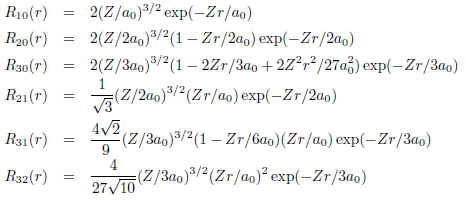
\includegraphics{Images2/foncrad.PNG}
    \caption{Fonctions radiales}
    \label{fig:foncrad}
\end{figure}
On remarque que les fonctions d'onde s ont une amplitude non nulle en $r = 0$, contrairement aux fonctions
d'onde des états $l\neq 0$ qui se comportent en $r^l$ près de l'origine. C'est le potentiel centrifuge $l(l+1)\hbar^2/2\mu r^2$ qui empêche l'électron de pénétrer dans le noyau. Pour une même valeur de n, les états de plus bas $l$ ont une amplitude plus importante près de $r = 0$.

À le figure \ref{fig:fcx_rad_1} sont représentées les fonctions d'onde radiales ($R_{nl}$) et fonctions de distribution radiales ($D_{nl}(r)=r^2|R_{nl}(r)|^2$) (qui est la probabilité par unité de longueur de trouver l'électron à une distance $r$ du noyau) de quelques états de l'atome d'hydrogène ($Z=1$):
\begin{figure}[htp]
    \centering
    \includegraphics[scale=0.8]{Images2/ex.PNG}
    \caption{Fonctions d'onde radiale et de distribution radiale des 4 premiers états s. Le nombre de noeuds est $n-1$}
    \label{fig:fcx_rad_1}
\end{figure}
Quelques remarques à propos de ces figures:

\begin{itemize}[label=$\bullet$]
    \item Si on veut savoir quelle est la probabilité que l'électron se trouve à une distance $r$ du noyau, il faut prendre le carré de la fonction d'onde et intégrer sur le volume, cette probabilité de trouver l'électron dans une coque sphérique comprise entre $r$ et $r+\dif r$ est donc $r^2|R_{nl}(r)|^2\dif r\int \dif\Omega |Y_{lm}(\theta,\phi))|^2$. Il y aura donc apparition d'un facteur $r^2$ venant des coordonnées sphériques. Ce qu'on va calculer c'est donc la densité radiale de probabilité. L'intégrale porte aussi bien sûr sur la partie angulaire de la fonction d'onde mais ce n'est pas ce qui nous intéresse. La densité radiale est en fait la probabilité de présence à une certaine distance $r$ du noyau.
    \item Dans un état 1s, l'électron se trouve à une distance moyenne d'un rayon de Bohr, par définition. Sa distribution est centrée à une unité atomique.
    \item Dans l'état 2s, la majeure partie de la probabilité se trouve à plus grande distance que pour l'état 1s. De 1 u.a. (pour 1s), on est passé à environ 4 u.a. (pour 2s).
    \item Le nuage électronique s'étend rapidement au fur et à mesure que $n$ augmente (évolution en $n^2$)
    \item La courbe de distribution radiale de l'état 1s montre un confinement tout près de $r=0$.
    \item On remarque la présence de lobes sur les courbes, le nombre changeant avec le moment angulaire: en effet les fonction radiales dépendent de $l$.
    \item Les polynômes de Laguerre ont un indice $n-l-1$ et cet indice indique le nombre de noeuds de la fonction.
\end{itemize}

Les figures \ref{fig:fcx_rad_2} et \ref{fig:fcx_rad_3} sont quelques représentations des fonctions d'onde et distributions radiales pour d'autres états.

\begin{figure}[htp]
    \centering
    \includegraphics{Images2/p.PNG}
    \caption{Fonction d'onde radiale et fonction de distribution radiale des 4 premiers états p (courbe 2p bien centrée à 4 rayons de Bohr). La courbe noir correspond à 2p et la courbe bleue à 5p}
    \label{fig:fcx_rad_2}
\end{figure}

\begin{figure}[htp]
    \centering
    \includegraphics{Images2/spdf.PNG}
    \caption{Fonction d'onde radiale et fonction de distribution radiale des états 4s, 4p, 4d et 4f. Le nombre de noeuds est $4-l-1$}
    \label{fig:fcx_rad_3}
\end{figure}

Les états de moment angulaire maximum ($l=n-1$) sont beaucoup plus simples à comprendre que les autres qui ont un comportement ondulatoire (présence de noeuds et ventres dans leur fonction d'onde). En effet, l'électron peut être vu comme une onde piégée dans un potentiel qui va, sous l'action de ce dernier, former une espèce d'onde stationnaire : ce sont les noeuds et les ventres que l'on observe (L'électron a une probabilité de présence nulle sur un noeud et une probabilité forte sur un ventre). On peut donner une image assez classique de ces noeuds et ventres. Lorsqu'on a des noeuds et des ventre, on peut voir l'électron comme une onde stationnaire qui fait des aller-retours entre le noyau et le bord du potentiel. Cependant, lorsque $l$ est maximal (i.e. $l=n-1$), la partie radiale de la fonction d'onde $R_{n,l=n-1}$ ne présente plus qu'un seul ventre sans noeuds. Dès lors, on doit ainsi plus voir l'électron comme orbitant à une distance moyenne constante du noyau. Attention que ceci est une image fort classique pour la mécanique quantique. Cependant plus $n$ est grand, plus on se rapproche de cette image et on peut donc considérer l'électron comme étant une particule classique orbitant autour d'un noyau (surtout à partir de $n=100$).

Plus le nombre quantique $n$ d'un état est élevé, plus l'état correspondant est excité. Un état de grand $n$ est appelé état de Rydberg. A l'échelle atomique, la fonction d'onde d'un tel état s'étend sur de très grandes distances, comme suggère l'expression du maximum de la fonction de distribution radiale

\[
    r\eq \dfrac{n^2}{Z}a_{\mu}
\]
Par exemple, la fonction d'onde radiale de l'état 50s qui est représentée figure \ref{fig:50s} s'étend jusque $5000a_0= \SI{0.27}{\mu m}$.

\begin{figure}[htp]
    \centering
    \includegraphics{Images2/50s.PNG}
    \caption{Fonction d'onde radiale réduite de l'état 50s}
    \label{fig:50s}
\end{figure}





\newpage

\section{Systèmes à électrons non appariés}
\subsection{Introduction : les alcalins}

Les alcalins sont les éléments de la première colonne du tableau périodique. Ils ont une structure électronique à coeur de gaz rare. Ils perdent facilement leur électron de valence célibataire dans la sous-couche externe s. Nous avons par exemple:

\begin{center}
    Li [He:1s$^{2}$] 2s \\
    Na [Ne: 1s$^{2}$2s$^{2}$2p$^{6}$] 3s \\
    K [Ar: 1s$^{2}$2s$^{2}$2p$^{6}$3s$^{2}$3p$^{6}$] 4s
\end{center}
Pour chaque sous-couche pleine, on rappelle qu'on a $\sum_i l_i = 0$.

Nous allons essayer de décrire ces atomes comme un atome d'hydrogène. Tout d'abord, nous nous intéressons au lithium. Dans cette approche de l'atome d'hydrogène on peut voir l'électron 2s comme lié à un ion Li$^{+}$ que l'on peut considérer approximativement comme un proton dans le sens où c'est une charge positive. Puisque c'est un électron 2s, nous savons qu'il a une probabilité de présence non-nulle près du noyau, c'est-à-dire dans le volume occupé par les deux autres électrons.


Étant donné que tout cela est probabiliste, il se peut que l'électron 2s se trouve plus proche du noyau que les autres électrons ("plus proche" d'une façon tout à fait schématique) et que donc il "voit" une charge qui n'est pas $1e$ mais $2e$ ou $3e$ car il n'y a plus d'effet d'écrantage.

Nous avons donc $Z$ qui augmente et l'énergie de liaison $E_n \propto 1/n^2$ aussi. Nous corrigeons par conséquent le nombre quantique principal qui n'est donc plus un nombre entier. Cette correction s’appelle le \textbf{défaut quantique}, notée $\delta_l$, et c’est une bonne solution pour décrire la perturbation de ces électrons dits externes lorsque nous faisons varier le nombre quantique principal.
Le défaut quantique sera toujours du même ordre de grandeur pour tous les alcalins car il ne dépend pas de $n$ mais seulement de $l$. En effet, la probabilité de présence près du noyau de l'électron diminue avec l'augmentation de $l$, donc le défaut quantique sera plus grand pour les plus petits $l$. Pour des moments angulaires plus importants ($l$ élevé), le potentiel effectif (dû au terme centrifuge) va empêcher les électrons externes d’aller à courtes distances et donc ils ne seront pas perturbés par la présence des autres électrons.

\[
    \delta_s>\delta_p>\delta_d>\delta_f\simeq 0
\]
L'énergie de liaison des alcalins obéit à la loi de Balmer modifiée par l’introduction du défaut quantique, qui rend compte de l’écrantage imparfait de la charge du noyau par les autres électrons. Il est d’autant plus grand que l’orbitale a une grande probabilité de présence à courte distance.

\begin{equation}
    E_{nl} \eq  - \dfrac{Ry}{2(n-\delta_l)^2}
    \label{eq:def_quant}
\end{equation}

NB: pas de facteur 2 au dénominateur quand on est en eV ; on est en Hartree dans cette formule.


Si nous nous intéressons maintenant au cas du sodium nous constatons que la correction dépasse 1 pour $l=0$ : $\delta_l = 1.35$. Cela signifie que le remplissage des couches ne se fera pas suivant la règle de Madelung (ou  Klechkowski). \textcolor{red}{Sûr de ça? Parce qu'il y a aussi l'effet joué par la correction du terme $l=1$ à prendre en compte si on veut `classer' les couches}
En effet, pour le potassium (K) par exemple, le 3 de la sous-couche 3d devient 2.75 tandis que le 4 de la sous couche 4s devient 1.81. Par conséquent, l’énergie de la 4s est plus petite que celle du 3d comme l'indique la formule \ref{eq:def_quant}. La sous-couche 4s sera donc remplie avant la 3d.

Ce phénomène ne se limite pas seulement aux alcalins. Pour  n'importe quel atome excité nous pouvons calculer le défaut quantique. (cf exercice sur l'hélium vu en TP).




\subsection{Rayon X}
\subsubsection{Contexte et rappels}


Nous allons ici développer un outil très important pour l'identification des éléments. Il a notamment servi à identifier la présence d'éléments terrestres dans le Soleil, ce qui n'avait a priori rien d'évident. En bombardant un matériau d'électrons de haute énergie, on observe l'émission de rayons X caractéristiques de sa structure.\\

Dans un atome à plusieurs électrons, nous savons que l'énergie ne suit plus exactement la loi de Balmer obtenue pour l'atome d'H ($E_n \propto Z/n^2$). En effet, il y a un effet dû aux autres électrons. Comme nous l'avons vu, cet effet peut être pris en compte en considérant un `défaut quantique' (formule \ref{eq:def_quant}). Cependant, une autre façon de voir les choses est d'utiliser une charge effective mais de laisse le nombre quantique inchangé. Cette charge effective $Z^{*}$ perçue par chaque électron est définie comme \[ Z^{*}=Z-\sigma \] où $\sigma$ représente l'effet d'écran produit sur l'électron d'intérêt par les électrons plus proches du noyau. Dès lors, l'énergie s'exprime comme

\begin{equation}
    E_n \eq -\dfrac{1}{2} \dfrac{(Z-\sigma_n)^2}{n^2} \; [\si{ua} = \si{Ha}]
    \label{eq:energie_effective}
\end{equation}
Comme vu dans l'introduction, lors du passage d'un électron de haute énergie dans un milieu matériel, l'électron subit une perte d'énergie continue sous forme de rayonnement de freinage (pour de hautes énergies de l'électron incident, on peut ignorer la perte sous forme d'ionisation, voir figure \ref{fig:Résumé pertes}). La figure idéalisée de ce rayonnement selon la longueur d'onde de l'électron incident\footnote{On observe donc bien entendu pour un même électron une variation de cette longueur d'onde au cours de sa progression.} se trouve à la figure \ref{fig:Freinage idéalisé} où l'\textit{intensité relative} correspond à l'intensité du rayonnement, autrement dit $\fdif{E}{x}$ la perte d'énergie par unité de distance pour l'électron [\si{J/m}].

\begin{figure}[htp]
    \centering
    \includegraphics[scale=0.8]{Images2/RésuméPerte.PNG}
    \caption{Perte d'énergie par unité de longueur en fonction de l'énergie incidente. On a ici représenté les 2 effets de perte d'énergie dans un matériau : le rayonnement de freinage et la perte par ionisation}
    \label{fig:Résumé pertes}
\end{figure}%
\begin{figure}[htp]
    \centering
    \includegraphics[scale=1.0]{Images2/FreinageIdéalisé.PNG}
    \caption{Rayonnement de freinage sans phénomène de résonance avec les atomes de la cible}
    \label{fig:Freinage idéalisé}
\end{figure}%

Dans la réalité, la perte d'énergie par unité de longueur en fonction de la longueur d'onde incidente est du type de la courbe représentée à la figure \ref{fig:Rayonnement freinage} (et non de la courbe représentée à la figure \ref{fig:Freinage idéalisé} qui n'est qu'une approximation négligeant complètement un phénomène important). Ainsi, pour des longueurs d'onde particulières, la perte d'énergie est drastiquement augmentée. Le phénomène responsable de cette perte drastique est dû à la résonance entre l'énergie de l'électron incident et (dans notre cas présent) des électrons de coeur : l'énergie perdue par les électrons lors de cette résonance correspond à l'énergie des photons associés aux rayons X observés dont nous discuterons dans un instant.\\
\begin{figure}[htp]
    \centering
    \includegraphics[scale=1.0]{Images2/RayonnementFreinage.PNG}
    \caption{Rayonnement de freinage avec résonance avec les niveaux profonds des atomes cibles}
    \label{fig:Rayonnement freinage}
\end{figure}


\subsubsection{Émission de rayons X}


Les fréquences auxquelles on observe les phénomènes de résonance dans le spectre du rayonnement de freinage (= les fréquence où on a des pics d'absorption) correspondent aux fréquences des transitions d'orbitales $n = 2$ vers $n = 1$. Pour caractériser ces transitions, on peut se servir de la loi empirique de Moseley, qui n'est qu'une généralisation des différentes séries de Lyman, Balmer, etc\footnote{En fait, on peut l'obtenir en faisant simplement la différence entre deux niveaux d'énergie distincts via la formule \ref{eq:energie_effective} où on considère un écrantage `moyen' (=la moyenne des écrantages des deux niveaux dont on fait la différence)}.
\begin{equation}
    h\nu
    \eq E_{n_1} - E'_{n_2}
    \eq \dfrac{1}{2}(Z-\sigma_{n_1})^2\left(\dfrac{1}{n_1^2}-\dfrac{1}{n_2^2}\right)
    \label{eq:Moseley}
\end{equation}

Mais dis-moi Jamy, pourquoi est-ce que les atomes émettent ces rayons X? Hé bien Fred, c'est très simple : lors du passage de la particule incidente dans l'atome, on va observer des chocs entre elle et les électrons de coeur (de $n=1$ voire $n=2$) qui sont fortement liés au noyau (en effet, les électrons proche du noyau ne subissent aucun effet d'écrantage atténuant l'action du noyau). Ces chocs avec les électrons de coeur entraînent des trous dans la couche qui sera comblé par la transition d'un électron d'un couche de $n$ plus élevé ($n=2$ sur la figure \ref{fig:Rayons X}). Le rayon X est donc l'émission qui s'associe au passage de l'électron d'une orbitale d'un $n$ élevé à l'orbitale de coeur qui a perdu un électron.
\begin{figure}[htp]
    \centering
    \includegraphics[scale=0.8]{Images2/Rayons X.PNG}
    \caption{Schéma de l'émission de rayons X suite à une ionisation de coeur.}
    \label{fig:Rayons X}
\end{figure}
Grâce aux rayons X, on peut calculer l'effet d'écran d'un certaine couche, c'est-à-dire "de combien la charge du noyau diminue quand on se trouve au-delà de cette couche et donc que les électrons de cette couche agissent comme un écran?". Lors d'une ionisation depuis $n=1$, on a deux électrons dans la couche s1 et donc l'écrantage est approximativement 2. Après ionisation, il ne reste plus qu'un seul électron dans cette couche et par conséquent l'effet d'écran n'est plus que 1 approximativement : Z est à peu près diminué de 1. Ainsi, l'ionisation a bien diminué l'effet d'écran de 1.\\
Pour ce qui est des ionisations de la couche (complète : 8 électrons) $n=2$, on observe après ionisation un effet d'écran de 7.4 dans cette couche de 7 électrons, ce qui est cohérent. Ces valeurs de correction ont été découvertes empiriquement (cfr. l'équation de Moseley \ref{eq:Moseley}).
On calcule donc les fréquences des photons associées aux transitions $2\rightarrow1$ et $3\rightarrow2$:
\[
    \nu_{12}
    \eq \nu_{K_\alpha}
    \eq k (Z - 1)^2 \;[Hz]
\]
\[
    \nu_{23}
    \eq \nu_{L_\alpha}
    \eq k' (Z - 7.4)^2 \;[Hz]
    \;\approx\;  k' (Z - 7)^2 \;[Hz]
\]
où $k$ et $k'$ sont des constantes numériques issues de la formule \ref{eq:Moseley}.



\subsubsection{Émission d'électrons \emph{Auger}}



On sait par la formule \ref{eq:Moseley} que la différence d'énergie entre le seuil d'ionisation et le niveau $n = 2$ est toujours inférieure à la différence d'énergie entre les niveaux 1 et 2. Intéressons-nous à l'émission des "électrons Auger", comme représenté à la figure \ref{fig : Auger}. En fait, lorsqu'un rayonnement ionisant ionise l'électron $1s$, les électrons des couches externes vont venir boucher ce trou en émettant des rayons X. Or, comme rappelé au début de ce paragraphe, l'énergie entre 1s n'importe quel autre niveau est supérieure à l'énergie d'ionisation d'un électron d'un niveau de $n>2$.

Dès lors, dans notre exemple à la figure \ref{fig : Auger}, le rayon X libéré par l'électron $^2P_{1/2}$ a une énergie suffisante pour ioniser l'autre électron $^2P_{1/2}$. Cet autre électron, ionisé, est appelé "électron Auger" et peut en pratique se situer n'importe où ailleurs dans l'atome (il ne se trouve pas forcément au même terme que l'électron qui bouche la couche 1s). Ainsi, on se retrouve avec un atome ayant perdu 2 électrons au total. En outre, on peut avoir 3 électrons manquant à la fin si le rayonnement provoqué par l'ionisation de l'électron Auger ionise encore un autre électron (ce phénomène est moins intense cependant).

Il est dès lors probable que, à la place d'émettre un rayon X, notre atome émette un électron. Cette électron émis aura l'énergie du rayon X (qui est la différence entre les niveaux d'énergie) diminuée du potentiel d'ionisation. On peut ainsi observer un spectre de fréquence à la figure \ref{fig:SpectreAuger} pour ces électrons émis, et ce spectre est structuré de la même façon que le spectre d'émission des rayons X. En fait, la seule différence entre le spectre d'émission d'électrons et le spectre d'émission de rayons X par un atome soumis à un rayonnement ionisant est le potentiel d'ionisation : les électrons doivent effectuer un travail pour sortir de la matière, contrairement aux photons.
\begin{figure}[htp]
    \centering
    \includegraphics[scale=0.8]{Images2/Auger.PNG}
    \caption{Schéma de l'émission d'électrons Auger suite à une ionisation de coeur.}
    \label{fig : Auger}
\end{figure}
\begin{figure}[htp]
    \centering
    \includegraphics[scale=1.0]{Images2/Spectre Auger.PNG}
    \caption{Spectre en fréquence des électrons Auger}
    \label{fig:SpectreAuger}
\end{figure}








\subsection{Le laser}

\subsubsection{Émission spontanée, émission et absorption stimulés}




On détaille ici les équations qui gouvernent ces phénomènes. L'analogie avec la cinétique chimique pour des réactions d'ordre 1 ou la radioactivité est directe. "Un atome ne vieillit pas" et un état non plus, la probabilité de transition par unité de temps est donc une constante.\\
Nous allons donc dans cette section décrire les différents phénomènes d'émission et d'absorption à l'aide d'équations différentielles. Nous allons également utiliser des taux de transitions $A_{ij}$ et $B_{ij}$ (= probabilité de transition par seconde) tel que $i$ est l'état de départ et $j$ l'état d'arrivée.
\begin{figure}[htp]
    \centering
    \includegraphics[scale=0.8]{Images2/Emission Spontanée.PNG}
    \label{fig:emission_spont}
\end{figure}
où $N_2(t)$ est la population atomique dans l'état d'énergie $E_2$.
\begin{figure}[htp]
    \includegraphics[scale=0.85]{Images2/Absorption stimulée.PNG}
    \label{fig:absorb_stimul}
\end{figure}
\begin{figure}[htp]
    \includegraphics[scale=0.9]{Images2/Emission stimulée.PNG}
    \label{fig:emission_stimul}
\end{figure}
Avant de continuer, quelques remarques :
\begin{itemize}[label=$\bullet$]
    \item L'émission `spontanée' n'existe pas vraiment. En effet, il faut toujours qu'il y ait une excitation qui pousse un électron à émettre un rayonnement. Ce qu'on dénote par "émission spontanée" est l'émission d'un photon par l'électron sous une excitation interne à l'atome (pas de photon externe à l'atome venant l'exciter). Ces photons "internes" sont les photons du champ E : selon la QED, le champ EM est composé de photons virtuels et ce sont ces photons virtuels qui excitent nos électrons.
    \item L'émission stimulée, bien que contre-intuitive, découle simplement de la micro-réversibilité de l'absorption stimulée : Einstein savait que la physique aimait la "micro-réversibilité" et il devait par conséquent avoir un phénomène opposé à l'absorption stimulée.
    \item Pour ce qui est des émissions (stimulée comme spontanée), on se rend bien compte que la solution à l'équation différentielle sera une exponentielle décroissante avec le temps. D'une certaine population, on va avoir une atténuation exponentielle avec un temps de vie caractéristique qui est l'inverse de la constante $A_{ij}$ ou $B_{ij}$. Ceci n'est valide que lorsqu'on a uniquement de l'émission stimulée ou uniquement de l'émission spontanée.
    \item On a ici décomposé l'élément de la matrice de perturbation associé aux états concernés $W_{ij}(\nu)$ en un facteur indépendant de l'onde incidente $B_{ij}$ et la densité d'énergie incidente $\rho(\nu)$.
    \item On a pas de relation à ce stade entre $B_{12}$ et $B_{21}$.
\end{itemize}
On peut exprimer, de manière tout à fait générale, l'évolution des populations\footnote{le terme `population' désigne le nombre de particules dans un certain état dans un système. Plus précisément on parle dans notre cas d'une population d'électrons ayant la même énergie dans un gaz macroscopique par exemple} en fonction des taux de transition ($A_{ij}$ et $B_{ij}$) et de la densité énergétique ($\rho(\nu)$).\\
En effet, dans un système à deux états, l'évolution de la population $N_1$ est dictée par son approvisionnement depuis l'état 2 (émissions spontanée et stimulée) en même temps que sa dépopulation pour aller vers l'état 2 (absorption stimulée):
\begin{equation}
\boxed{
    \fdif{N_1}{t}
    \eq  [B_{21}\rho(\nu) + A_{21}]N_2 \;-\; B_{12} \rho(\nu)N_1
    }
    \label{eq:N2}
\end{equation}
De façon tout à fait équivalente pour $N_2$, la population de l'état 2:
\begin{equation}
\boxed{
    \fdif{N_2}{t}
    \eq - [A_{21} + B_{21} \rho(\nu)]N_2 \;+\; B_{12}\rho(\nu)N_1
    \label{eq:N1}
    }
\end{equation}
En sommant les équations \ref{eq:N1} et \ref{eq:N2}, on observe bien la conservation du nombre de particules (du nombre d'électrons pour nous). Ceci se généralise très facilement lorsqu'on a plus que 2 états.
\begin{equation}
\boxed{
    \fdif{N_1}{t}\;+\;\fdif{N_2}{t} \eq 0
    }
\end{equation}



\subsubsection{L'équilibre thermodynamique}



Grâce à la théorie quantique du corps noir (on n'a plus l'évolution en $T^4$ de l'intensité en fonction de la longueur d'onde), on peut écrire l'expression de la densité énergétique \textbf{à l'équilibre thermodynamique} émise par une matière chauffée à une température $T$ donnée en fonction de la fréquence émise $\nu$.
\begin{equation}
    \rho(\nu) \eq \dfrac{8\pi h \nu^3}{c^3(\exp(\dfrac{h\nu}{k_BT})-1)}
\end{equation}
\begin{figure}[htp]
    \centering
    \includegraphics[scale=1.1]{Images2/corps_noir.png}
    \caption{Spectre d'un corps noir à divers températures}
    \label{fig : Corps noir}
\end{figure}
Nous savons que la répartition entre les états 1 et 2 doit respecter la distribution de Maxwell-Boltzmann en prenant en compte les dégénérescences en énergie. Ces dégénérescence sont notées $g_1$ et $g_2$. L'excitation depuis l'état fondamental 1 vers l'état excité 2 qui est plus probable se fait thermiquement (via l'énergie $k_BT$) et est d'autant plus probable que $h\nu$, la différence d'énergie entre l'état 1 et l'état 2, est petite :
\[
    N_2 \eq \dfrac{g_2}{g_1} \; \exp\left(\dfrac{-h\nu}{k_BT}\right) \;N_1
\]
En partant des conditions d'équilibre thermodynamique et en substituant, on obtient :
\[
    \fdif{N_1}{t} \eq \fdif{N_2}{t} \eq 0
\]
\[
    \fdif{N_2}{t}
    \eq 0
    \eq - \left[\;A_{21} + B_{21} \rho(\nu) + B_{12}\rho(\nu) \dfrac{g_1}{g_2} \; \exp\left(\dfrac{h\nu}{k_BT}\right) \;\right] N_2
\]
\[
    \rho(\nu)
    \eq \dfrac{A_{21}}{B_{12}\rho(\nu) \cdot \dfrac{g_1}{g_2} \exp(\dfrac{h\nu}{k_BT}) - B_{21}}
    \;\equiv\; \dfrac{8\pi h \nu^3}{c^3\left(\exp(\dfrac{h\nu}{k_BT})-1\right)}
\]
Cette dernière égalité n'est pas triviale : en effet, nous égalisons la densité d'énergie classique obtenue avec la théorie du corps noir et la densité d'énergie du rayonnement. On peut aisément comprendre cette égalité en considérant le gaz compris dans un corps noir : à l'équilibre thermodynamique, l'énergie thermique transmise de la paroi à nos atomes est égale à l'énergie émise par rayonnement des atomes.\\
En isolant les taux de transition, on obtient ces deux relations qui seront très utiles.
\begin{equation}
    B_{21} \eq \dfrac{g_1}{g_2}B_{12}
    \label{eq:equilire1}
\end{equation}
\begin{equation}
    \dfrac{A_{21}}{B_{21}}
    \eq \dfrac{8\pi h \nu^3}{c^3}
    \eq \dfrac{\hbar \omega^3}{\pi^2c}
    \label{eq:equilire2}
\end{equation}
On remarque donc que pour un $A_{21}$ important par rapport à $B_{21}$, l'émission de lumière ultraviolette est bien plus probable que l'émission d'infrarouge.


\subsubsection{Principe de fonctionnement du LASER et inversion de population}



\begin{figure}[htp]
    \centering
    \includegraphics[scale=0.7]{Images2/Laser.png}
    \caption{Schéma d'un laser à hélium-néon}
    \label{fig:Laser}
\end{figure}
Le concept du laser est relativement simple : en se servant de l'émission stimulée, on met en place une réaction en chaîne qui transformera l'énergie fournie au système (via le courant créé par les électrodes) en émission de lumière dans une gamme extrêmement précise de fréquences. En pratique, l'amplification se fait dans la chambre à gaz, la lumière se propage selon l'axe $z$ jusqu'à un miroir à 99\% qui permet de laisser sortir une partie du faisceau (celle dont on se sert) et de réfléchir le reste dans le système pour à nouveau l'amplifier.

On s'était permis plus tôt une hypothèse simplificatrice que l'on ne peut conserver : on avait supposé que les états absorbaient de la lumière à toutes les fréquences. C'est le cas pour un solide cristallin possédant suffisamment d'états (de degrés de liberté) mais c'est faux pour un gaz dont les fréquences d'absorption sont celles des atomes : il n'y a pas de forme macroscopique dans un gaz pour créer beaucoup de niveaux d'énergie. Pour remédier à cela, nous introduisons une fonction $g(\nu - \nu_0)$ qui doit représenter l'atténuation de la stimulation dès qu'on s'éloigne de la fréquence de résonance $\nu_0$. On repart des équations \ref{eq:N1} et \ref{eq:N2} et des relations qu'on a trouvées grâce à l'équilibre thermodynamique \ref{eq:equilire1} et \ref{eq:equilire2}. On réécrit cependant les taux de transition $A_{ij}$ et $B_{ij}$ avec $\tau_{sp}$, le temps de vie de l'état 2:
\[
    \dfrac{g_1}{g_2}W_{12} \eq W_{21}^{st} \eq B_{21} \rho(\nu) g(\nu - \nu_0)
\]
\[
    W_{21}^{sp} \eq A_{21} \eq \dfrac{1}{\tau_{sp}} \eq \dfrac{8\pi \nu^3}{c^3}B_{21}
\]
\[
    W_{21}^{st} \eq \dfrac{c^3}{8\pi h \nu^3}\dfrac{\rho(\nu) g(\nu - \nu_0)}{\tau_{sp}}
\]
Intéressons-nous maintenant au rayon qui traverse notre gaz. On peut facilement imaginer que le phénomène d'amplification aura une forme exponentielle : une réaction émet $x$ photons qui donneront lieu à $x$ émissions stimulées.\\

On définit un facteur d'amplification $\gamma\ [\si{m^{-1}}]$, un gain qui représentera le comportement de notre faisceau le long de l'axe z (ou, de façon équivalente, au cours du temps via $c\dif t = \dif z$). On exprime également l'intensité lumineuse $I\ [\si{W/m^2}]$ comme un flux d'énergie à travers une surface, ce qui revient à multiplier la densité énergétique $\rho(\nu)\ [\si{J/m^3}]$ par la vitesse de propagation $c\ [\si{m/s}]$:
\[
    \fdif{I_\nu}{z} \eq \dfrac{\dif I_\nu}{c\dif t} \eq \gamma I_\nu
\]
\[
    I_\nu(z) \eq I_\nu(0) e^{\gamma z} \eq c\rho(\nu)
\]
%pas sûr d'avoir très bien compris comment intégrer la dépendance en z dans l'expression avec rho mais grosso modo c'est ça
On a ici négligé l'émission spontanée, elle a pourtant bien lieu mais son caractère isotrope l'empêche de contribuer significativement au mécanisme. Il s'agit néanmoins d'une limitation technique qui entraîne une perte pour le système en fonctionnement.
Pour avoir un gain, il nous faut donc une augmentation du nombre de photons, on exprime donc la variation du nombre de photons par unité de volume [\si{1/m^3}], $N_{ph}$, au cours du temps. On a deux contribution à la variation de $N_{ph}$ : l'émission depuis l'état 2 vers l'état 1 (terme positif) et l'absorption depuis l'état 1 vers l'état 2 (terme négatif).
\[
    \fdif{N_{ph}}{t}
    \eq N_2 W_{21}^{st} - N_1 W_{12}
    \eq W_{21}^{st} (N_2 - \dfrac{g_2}{g_1}N_1)
\]
La variation de la densité énergétique au cours du temps est la variation du nombre de photons multipliée par l'énergie d'un photon. On passe ensuite à l'intensité via la vitesse de propagation $c$.
\begin{align*}
    \dfrac{1}{c}\fdif{I}{t}
    &\eq  \fdif{\rho}{t}\\
    &\eq  h\nu\fdif{N_{ph}}{t}\\
    &\eq  h\nu (N_2 - \dfrac{g_2}{g_1}N_1) \dfrac{c^3}{8\pi h \nu^3}\dfrac{\rho(\nu) g(\nu - \nu_0)}{\tau_{sp}}\\
    &\;\equiv\;  c\rho(\nu)\gamma
\end{align*}
En définitive, nous obtenons l'expression suivante pour le facteur d'amplification $\gamma$ :
\begin{equation}
    \boxed{
        \gamma \eq \dfrac{c^2}{8\pi\nu^2}\dfrac{g(\nu - \nu_0)}{\tau_{sp}}(N_2 - \dfrac{g_2}{g_1}N_1)
    }
\end{equation}
\[
\boxed{
    \gamma > 0 \; \longrightarrow \; \dfrac{N_1}{g_1} < \dfrac{N_2}{g_2}
    }
\]
On s'aperçoit donc que pour avoir une amplification du faisceau, il nous faut inverser les populations 1 et 2\footnote{Selon Wikipédia, \textit{une inversion de population se produit lorsqu'un système [...] se trouve dans un état dans lequel la majorité des éléments sont dans un état excité plutôt que dans leur état fondamental}}. Augmenter le courant ne ferait qu'échauffer le gaz qui suit la distribution de Maxwell-Boltzmann : cette dernière contraint la population de l'état fondamental à être au moins autant peuplée que tout autre état\footnote{Pour s'en convaincre, on peut se souvenir du modèle à deux états de la physique statistique pour lequel une température infinie entraîne une probabilité d'occupation de $\dfrac{1}{2}$ pour chaque état.}. On va donc devoir tricher.


\subsubsection{L'inversion de population en pratique}


La subtilité réside ici dans les petits termes en bas du contrat : cette limitation n'est valable en l'état que pour un système homogène\footnote{Sous-entendu : composé d'un seul type de corps}. On va donc choisir un mélange de gaz pour remplir notre laser, et comme souvent en science on ne va pas faire les choses au hasard.\\

Pour expliquer l'inversion de population, l'auteur, dans sa grande sagesse, a choisi une analogie claquée au sol. Imaginons avoir un escalier et un ensemble de billes. Imaginons que par la décision d'un Dieu mesquin ou d'une loi de la Nature quelconque, le nombre de billes par marche aille toujours décroissant alors qu'on monte dans les marches. Autrement dit, pour toute marche, la marche supérieure doit toujours contenir moins de billes (ou autant) que la marche du dessous.

\begin{figure}[htp]
    \centering
    \includegraphics[scale=1.0]{Images2/escalier2.jpg}
    \caption{Un joli petit escalier}
    \label{fig:escalier}
\end{figure}
Imaginons maintenant que, bravant la volonté divine, on amène une échelle (= une grosse marche à côté de l'escalier) d'où l'on fait monter des billes. Dès lors, on se retrouve avec plus de billes sur la marche desservie par cette échelle que sur la marche d'en dessous : nous ne sommes plus à l'équilibre. Par conséquent, les billes vont tomber progressivement de marche en marche pour ré-obtenir la configuration d'équilibre recherchée : il y a plus de billes sur la dernière marche que sur l'avant-dernière. Nous avons ainsi obtenu une inversion de population grâce à notre échelle : nous avons réussi à avoir plus de billes dans un état excité (marche du haut) que dans un état fondamental (marche du bas).\\



Dans cette analogie, vous aurez compris que les marches représentent les niveaux d'énergie, les billes les électrons. Quand nous n'avions pas l'échelle, nous nous contentions d'exciter le système "par le bas" : seule l'excitation thermique (distribution de Maxwell-Boltzmann) nous permettait de faire monter les billes. Amener l'échelle est donc équivalent à un procédé qui permettrait d'amener en une fois les électrons à un niveau d'énergie bien supérieur. Ce procédé correspond au choc entre des atomes d'hélium chargés avec des atomes de néon.\\

L'Hélium étant un composé à faible Z, la différence d'énergie entre son fondamental et son premier état excité est nettement plus grande que la même différence pour le Néon. Lors du passage du courant à travers le gaz, l'Hélium s'excite donc naturellement à ce niveau (on amène donc les billes en haut de l'échelle). De son côté, le Néon subit également des excitations qui amènent des électrons à des niveaux supérieurs d'énergie mais conformément à la volonté de notre Dieu mesquin, marche par marche.

Or, les atomes de Néon subissent également des chocs avec les atomes d'Hélium de l'enceinte contenant le mélange des deux gaz. L'énergie est donc transférée de l'un à l'autre et amène des électrons du néon à de hauts niveaux d'énergie : on a notre inversion de population ! Il s'ensuit une \textbf{cascade radiative} qui ramène progressivement les électrons de l'Hélium à leur état fondamental. Pour donner la fin qu'elle mérite à cette analogie, on a mis en contact l'escalier de l'Helium (composés de hautes marches = échelles) à l'escalier du Néon (composé de petites marches) afin de provoquer l'inversion de population des billes dans le Néon. En tombant de marche en marche (voire plusieurs marches à la fois), les billes retombent dans leur état d'équilibre : cette descente est une cascade radiative.

Quantitativement, on a donc ici une émission de \SI{632.8}{nm}, ce qui correspond à une transition entre les états 1s$^2$2s$^2$2p$^5$5s et 1s$^2$2s$^2$2p$^5$3p.

\begin{figure}[htp]
    \centering
    \includegraphics[scale=1.0]{Images2/Escalier 1.png}
    \caption{Un joli petit escalier et une jolie petite échelle}
    \label{fig:Analogie}
\end{figure}
On a choisi pour ce laser le néon et l'hélium car le premier niveau d'excitation du second correspond très bien avec un état de haute énergie du second, la longueur de l'échelle correspond à une marche précise et haute de l'escalier en somme.\\
\begin{figure}[htp]
    \centering
    \includegraphics[scale=0.8]{Images2/hélium-néon.png}
    \caption{Schéma du fonctionnement du laser}
    \label{fig:schema_helium-neon}
\end{figure}



\newpage
\section{Transitions dipolaires}
\subsection{Expression du taux de transition}



Selon la théorie des perturbations dépendantes du temps au premier ordre\footnote{Voir le cours de MQ2 donné par Christophe Ringeval}, pour un système hydrogénoïde, le taux de transition $W$ (nous considérons un cas générique que nous appliquerons après à nos taux de transition $A_{21}$, $B_{12}$ et $B_{21}$) d'un état a d'énergie $E_a$ vers un état b d'énergie $E_b$ par absorption ou émission d'un photon de fréquence angulaire $w=|E_b-E_a|$ et sous une intensité $I$ est

\begin{equation}
    W\eq \dfrac{4\pi^2 \alpha \hbar}{m^2 w^2}I|M_{ba}|^2
\end{equation}
où $M_{ba}$ est l'élément de matrice de transition

\begin{equation}
    M_{ba}\eq \bra{\Psi_b}e^{-\imag\vec{k}\Cdot \vec{r}}\hat{\epsilon}\cdot\nabla \ket{\Psi_a}
    \label{Mba}
\end{equation}
où

\begin{itemize}[label=$\bullet$]
    \item $\vec{k}$ est le vecteur de propagation de l'onde
    \item $\hat{\epsilon}$ est le vecteur de polarisation
\end{itemize}
On peut tronquer le développement de Taylor de l'exponentielle

\begin{equation}
    e^{-\imag\vec{k}\Cdot\vec{r}}\eq 1-\imag\vec{k}\Cdot\vec{r}+\dfrac{1}{2!}(\imag\vec{k}\Cdot\vec{r})^2+...
    \label{eq:dvpl_expo}
\end{equation}
Si on garde seulement le premier terme de ce développement, on effectue ce qu'on appelle l'approximation dipolaire (physiquement, on néglige en fait les "effets de retard" à l'échelle de l'atome : si le photon a une longueur d'onde nettement supérieure à la taille de l'atome, tous les électrons de l'atome ressentiront le même champ E) et dans ce cas \eqref{Mba}, qu'on définit comme "le moment dipolaire dans la représentation de vitesse" devient
\[
    M_{ba} \;\simeq\; \bra{\Psi_b}\hat{\epsilon}\Cdot\nabla\ket{\Psi_a}
\]
De plus, on a que
\[
    m\vec{v}\eq \vec{p}\eq -\imag\hbar \nabla
\]
Donc
\[
    M_{ba} \simeq \dfrac{\imag m}{\hbar}\hat{\epsilon}\Cdot\bra{\Psi_b}\vec{v}\ket{\Psi_a}
\]
On sait aussi\footnote{Ceci vient directement de l'évolution de la valeur moyenne d'un opérateur au cours du temps : $\fdif{}{t}\langle A \rangle \eq \dfrac{1}{\imag\hbar}\langle[A,H] \rangle$} que $\vec{v}=\dot{r}=\dfrac{1}{\imag\hbar}[\vec{r},H_0]$ ce qui nous amène au moment dipolaire dans la représentation de longueur
\begin{align*}
    \bra{\Psi_b}\dot{\vec{r}}\ket{\Psi_a}
    &\eq
    \dfrac{1}{\imag\hbar}\bra{\Psi_b}\vec{r}H_0-H_0\vec{r}\ket{\Psi_a}\\
    &\eq
    \dfrac{1}{\imag\hbar}(E_a-E_b)\bra{\Psi_b}\vec{r}\ket{\Psi_a}\\
    &\eq
    \dfrac{1}{\imag\hbar}(-\hbar \omega)\bra{\Psi_b}\vec{r}\ket{\Psi_a} \\
    &\eq
    i \omega \bra{\Psi_b}\vec{r}\ket{\Psi_a} \\[5pt]
    \Longrightarrow \quad M_{ba} &\;\simeq\;
    -\dfrac{m \omega}{\hbar}\hat{\epsilon}\Cdot\bra{\Psi_b}\vec{r}\ket{\Psi_a}
\end{align*}
En remplaçant cette dernière expression de $M_{ba}$ dans l'expression du \textbf{taux de transition} $W$, on a
\[
    W\eq \dfrac{4\pi^2 \alpha}{\hbar}I |\hat{\epsilon}\Cdot\vec{r}_{ba}|^2
\]
On peut encore simplifier l'expression du taux de transition générique en prenant se valeur moyenne:
\[
    \int_{0}^{\pi/2} |\hat{\epsilon}\Cdot\vec{r}_{ba}|^2\sin{\theta} \dif\theta\eq |r_{ba}|^2\int_{0}^{\pi/2}\cos{\theta}^2\sin{\theta}\dif\theta\eq \dfrac{1}{3}|r_{ba}|^2
\]
Ainsi
\begin{equation}
    \overline{W}_{ba}\eq \dfrac{4\pi^2 \alpha}{3 \hbar}I |r_{ba}|^2
\end{equation}



    \subsection{Coefficients d'Einstein}



Les transitions radiatives sont caractérisées par les "coeffients d'Einstein", qui décrivent les taux de transition par émission spontanée $A_{2\Rightarrow1}$, émission stimulée $B_{2\Rightarrow 1}$ et absorption $B_{1\Rightarrow2}$.\\
Conformément aux équations \eqref{eq:equilire1} et \eqref{eq:equilire1}, ces coefficients sont donnés par

\begin{equation}
    B_{ba}\eq \dfrac{\overline{W}_{ba}}{\rho}\eq \dfrac{c\overline{W}_{ba}}{I}\eq \dfrac{4\pi^2 c \alpha}{3 \hbar}|r_{ba}|^2
\end{equation}

\begin{equation}
    A_{ba}\eq \dfrac{\hbar w^3}{\pi^2 c^3}B_{ba}\eq \dfrac{4 \alpha}{3 c^2}w_{ba}^3|r_{ba}|^2
\end{equation}





\subsection{Cas d'un atome à $N$ électrons}

Dans le cas d'un atome à $N$ électrons, le terme d'interaction radiative s'écrit :

\begin{equation}
    H_\text{rad}(t)\eq -\dfrac{\imag\hbar e}{m}\sum_{i=1}^{N} \vec{A}(\vec{r}_i,t).\nabla_i
\end{equation}
En unités atomiques, l'élément de matrice de transition dipolaire en représentation de longueur est ($\hat{\bm{\epsilon}}$ est, pour rappel, un vecteur) :

\begin{equation}
    M_{ba} \eq
    -\omega \hat{\bm{\epsilon}}\cdot\bra{\Psi_b}\sum_{i=1}^{N} \bm{r}_i\ket{\Psi_a}
    \eq
    -\omega \bra{\Psi_b}\hat{\bm{\epsilon}} \cdot \bm{D}\ket{\Psi_a}
    \eq
    -\omega \sum_{q=0,\pm 1}\bra{\Psi_b}\hat{\epsilon}_q^* D_q\ket{\Psi_a}
\end{equation}
où nous avons défini le vecteur $\bm{D}$, avec $i$ l'indice dénotant l'électron :

\[
    \bm{D} \;\equiv\; \sum_{i=1}^N \bm{r}_i
\]
et utilisé la définition du produit scalaire:

\begin{equation}
    \hat{\bm{\epsilon}}\Cdot \bm{r} \eq \hat{\epsilon}_xx + \hat{\epsilon}_yy + \hat{\epsilon}_zz \eq \sum_{q=0,\pm 1}  \hat{\epsilon}_q^* r_q
\end{equation}
L'opérateur $\bm{D}$ est un opérateur vectoriel, c'est-à-dire un opérateur tensoriel irréductible de rang 1. La généralisation des règles de sélection découle du théorème de Wigner-Eckart (qui, apparemment, découle de la théorie des groupes et qui est vachement long à démontrer donc on le prend comme acquis et on ne cherche pas vraiment à le comprendre) :

\begin{equation}
    \bra{\tau ` J'M'}D_q\ket{\tau JM}\eq \dfrac{1}{\sqrt{2J'+1}}\bra{\tau `J'}|\vec{D}|\ket{\tau J}\bra{J1Mq}\ket{J'M'}
\end{equation}
Les coefficients de Clebsch-Gordan sont donc nuls sauf si

\[
    J'\eq |J-1|, |J-1|+1, ..., J+1
\]

\[
    M+q\eq M'
\]

On a donc les règles de sélection pour une transition dipolaire électrique (E1):

\begin{equation}
    \Delta J\eq 0, \pm1 \quad \text{et} \quad \Delta M\eq 0, \pm 1 \quad \text{et        changement de parité}
\end{equation}


\newpage %je pense que c'est le mieux pour avoir les images au bon endroit (NP)
\subsection{Résumé des règles de sélection}

De façon tout à fait équivalente, mais en considérant le terme en $\vec{k}\Cdot\vec{r}$ dans l'équation \eqref{eq:dvpl_expo}, nous pouvons trouver les règles de sélection pour les transitions interdites. Tout ceci est fait dans le syllabus du Pr. Terao-Dunseath.


\begin{figure}[htp]
    \centering
    \includegraphics[scale=0.8]{Images2/regles.PNG}
    \caption{Règles de sélection des transitions radiatives}
    \label{fig:regles_transision_radiatives}
\end{figure}

\subsection{Diagramme de Grotrian}

Un diagramme de Grotrian indique les transitions permises entre les niveaux d'énergie des atomes. Il tient compte des règles de sélection liées aux changements de moment cinétique orbital et de spin des électrons.

\begin{figure}[htp]
    \centering
    \includegraphics[scale=0.5]{Images2/grotrian.PNG}
    \caption{Exemple de diagramme de Grotrian}
    \label{fig:grotrian}
\end{figure}





%-------------------------------------------- 2e Partie Urbain ----------------------------------------------
\newpage
\section{Hamiltonien spin-orbite et hyperfin}
\subsection{Hamiltonien spin-orbite}


L'électron possède un spin et un moment cinétique orbital. Nous avons donc une charge en mouvement, ce qui provoque un moment magnétique orbital. Ces deux moments magnétiques (de spin et orbital) interagissent ensemble et cette interaction est décrite pas l'hamiltonien de spin-orbite\footnote{D'où le <<SO>> du $W_\text{SO}$}, qui peut être traité comme une perturbation de l'hamiltonien $H_0$. L'hamiltonien associé à l'interaction du moment magnétique de spin avec le champ magnétique de l’électron en mouvement s'écrit

\[
    W_\text{SO} \eq  -\vec{\mu_\text{s}}\Cdot\vec{B}'
\]

avec $-\vec{\mu_\text{s}}$ le moment magnétique de spin. On rappelle les quantités suivantes:

\begin{enumerate}
    \item Moment magnétique créé par une boucle de courant :
    \[
        \vec{\mu} \eq \vec{I}\cross \vec{A} \eq -\dfrac{e\vec{v}}{2\pi r}\cross \pi r^2\hat{r} \eq -\dfrac{e}{2m}\vec{l}
    \]
    Attention : $\hat{r}$ désigne le vecteur $\dfrac{\vec{r}}{\abs{\vec{r}}}$ sa norme est donc égale à 1, $\vec{A}$ désigne le vecteur radial dont la norme représente la surface de la boucle de courant. On part de l'expression classique $\vec{\mu} = i\vec{S}$ où l'intensité $i = \dfrac{e|\vec{v}|}{2\pi r}$ et $S = \pi r^2$. Pour avoir un vecteur $\vec{S}$ perpendiculaire à la surface, on prend le produit vectoriel de $\vec{r}$ et $\vec{v}$. $\vec{l}$ est le vecteur moment orbital et s'écrit $m\vec{v}\cross\vec{r}$.
    \item Magnéton de Bohr et son implication pour le moment magnétique créé par une boucle de courant :
    \[
        \mu_\text{B} \eq \dfrac{e\hbar}{2m} \quad \Leftrightarrow \quad \vec{\mu} \eq -\mu_\text{B}\dfrac{\vec{l}}{\hbar}
    \]
    \item Par analogie à l'expression du moment magnétique créé par une boucle de courant (point au-dessus), nous pouvons écrire le moment magnétique de spin comme:
    \[
        \vec{\mu_\text{s}} \eq -g\mu_\text{B}\dfrac{\vec{s}}{\hbar} \qquad \textrm{avec } g=2.
    \]
    où nous avons utilisé le rapport gyromagnétique $g$, qui est défini comme étant \emph{le rapport entre le moment magnétique  et le moment cinétique d'une particule}.
    % utile le truc avec les unités?
    Pour mieux comprendre ce qu'on fait, on peut raisonner sur les unités : $\vec{\mu} = [\si{m^2kg/s}] = [\si{Js}]$. $\hbar$ a donc les unités d'un moment angulaire.
    \item Champ magnétique :
    \[
        \vec{B}' \eq \dfrac{\vec{B} - \vec{v}\cross \dfrac{\vec{E}}{c^2}}{\sqrt{1-\dfrac{v^2}{c^2}}} \simeq -\dfrac{\vec{v}\cross \vec{E}}{c^2}
    \]
    On ignore donc ici le boost de Lorentz lié à la correction relativiste.
    \item Champ électrique :
    \[
        \vec{E} \eq  -\dfrac{1}{e}\dfrac{\partial U}{\partial r}\hat{r}
    \]
\end{enumerate}

On peut donc réécrire l'interaction $W_\text{SO}$ comme suit,

\begin{equation}
    W_\text{SO} \eq  \dfrac{1}{2m^2c^2}\dfrac{1}{r}\dfrac{\partial U}{\partial r}(\vec{l}\Cdot\vec{s}) \eq  \zeta(r)\vec{l}\Cdot\vec{s}
    \quad\Longrightarrow\quad
    W_\text{SO}^{tot} \eq \sum_i\zeta(r_i)\vec{l_i}\Cdot\vec{s_i}
    \label{eq:Hamilt_SO}
\end{equation}

avec $\vec{l}$ le moment angulaire et $\sum_i...$ la somme sur les opérateurs mono-électroniques. Il y a différentes façons de dériver l’hamiltonien spin-orbite : on peut partir de l’équation de Dirac\footnote{Il s'agit d'une équation de Schrödinger relativiste pour les fermions, donc les électrons} ou alors traiter l’hamiltonien spin-orbite comme étant l’interaction du moment de spin, qu’on définit par analogie avec le moment magnétique d’une boucle de courant pour autant qu’on introduise le rapport gyromagnétique ($g$) à peu près égal à 2. A coté de ça, on a un champ magnétique $B$ qui est essentiellement causé par la présence d’un champ électrique dans le voisinage du noyau. Ce champ électrique pointe dans la direction radiale si on a un potentiel à symétrie centrale.\footnote{Ou alors on peut utiliser le raisonnement fait en quantique 2 en disant que c'est le proton qui tourne autour de l'électron et que le spin de l'électron interagit avec la champ magnétique créé par le noyau.}\\

Pour chaque électron, cette interaction spin-orbite est proportionnelle au produit scalaire du moment angulaire de cet électron et du spin de ce même électron (l'interaction spin-orbite concerne un électron et son propre moment angulaire). La fonction $\zeta(r)$ cache un peu tout ce qui va dépendre de la distance électron-noyau. Le facteur en $\dfrac{1}{r}$ implique que ce potentiel agit essentiellement au voisinage du noyau : l'interaction SO se passera donc surtout proche du noyau. Quand on a plusieurs électrons on va faire une somme.

Nous allons maintenant effectuer une approximation de l'expression \eqref{eq:Hamilt_SO} : nous allons remplacer la somme d’opérateurs mono-électroniques par le produit scalaire du moment angulaire total et du spin total. Étant donné que nous devons travailler en terme de $\vec{J}$ et non en terme de $\vec{L}$ ou $\vec{S}$, on va travailler avec des états de $\vec{J}$ total défini (pas de $\vec{L}$ ou de $\vec{S}$ défini). On peut donc passer d’une base à l’autre en réécrivant l’opérateur $\vec{L}\Cdot\vec{S}$.

\begin{equation}
    \vec{L}\Cdot\vec{S} \eq  \dfrac{1}{2}(J^2-L^2-S^2) \qquad \mathrm{avec} \quad \vec{J} \eq  \vec{L}+\vec{S}
    \label{eq:JLS}
\end{equation}
On se retrouve avec un élément de matrice de la forme donnée à l'équation \eqref{eq:Hamilt_SO_J1} où nous avons introduit un préfacteur $A(\gamma L S)$\footnote{Le $gamma$ représente les autres noöbres quantiques, si jamais on a un ECOC avec plus d'observables} qui cache la structure atomique mais qui est supposé représenter le facteur $\zeta(r_i)$. Nous avons donc une expression ne faisant plus intervenir que le moment angulaire total et non plus sur le moment angulaire de chaque électron.

\begin{align}
    \langle \gamma LSM_LM_S|H_\text{SO}|\gamma LSM_L'M_S' \rangle &\eq  A(\gamma LS)\langle \gamma LSM_LM_S|\vec{L}\Cdot\vec{S}|\gamma LSM_L'M_S' \rangle
    \label{eq:Hamilt_SO_J1}    \\
    &\eq
    \dfrac{1}{2}A(\gamma LS)\left( J(J+1)-L(L+1)-S(S+1)\right)
    \label{eq:Hamilt_SO_J2}
\end{align}
La formule \eqref{eq:JLS} nous permet d’écrire l'équation \eqref{eq:Hamilt_SO_J2}, et cette formulation nous permet d'établir la règle de Landé (cfr. figure \ref{fig:RegleLandé} où la colonne des $J$ est celle des états de structure fine) : pour une même valeur de $L$ et de $S$, l’écart en énergie entre le niveau $J$ et le niveau $J-1$ est proportionnel à $J$.

\begin{figure}[htp]
    \centering
    \includegraphics[scale=0.50]{Images2/regleLande.jpg}
    \caption{Règle de Landé.}
    \label{fig:RegleLandé}
\end{figure}

Donc il y a une première opération qui consiste à chercher les termes et vérifier que le terme de plus basse énergie est celui de multiplicité de spin la plus grande (règle de Hund). Ensuite, il faut encore coupler $\vec{L}$ avec $\vec{S}$ (pour obtenir $\vec{J}$) et pour un même couple $(L,S)$, on a les états de structure fine avec la correction de spin-orbite, sur lesquels on peut appliquer la règle de Landé.

En réalité, il existe d'autres corrections comme la monoconfiguration ou la correction au fait que nous avons considéré le moment angulaire total et le spin total au lieu des moments angulaires et de spin individuels (remplacement de la somme d'opérateurs monoélectroniques de l'équation \eqref{eq:Hamilt_SO}). Notre approximation a donc un impact sur la précision de la formule de Landé.

Mais on n’en a pas fini, il y a aussi la structure hyperfine! Nous avons donc pris en compte la correction de spin-orbite (couplage du moment magnétique de spin avec le moment magnétique orbital). Il nous reste à tenir compte de \textbf{l’interaction du spin du noyau, avec d'une part le spin des électrons, et d'autre part leur moment angulaire.}



\subsection{Hamiltonien hyperfin}

Nous allons ici considérer l'interaction du spin nucléaire, noté $\vec{I}$, avec d'une part le spin des électrons et d'autre part le moment magnétique des électrons. Pour commencer, et par analogie avec le moment magnétique de spin des électrons, notons le moment magnétique de spin du noyau (que nous couplerons après) :

\begin{equation}
    \vec{\mu_\text{I}}
    \eq -g_\text{I}\mu_\text{N}\dfrac{\vec{I}}{\hbar}
    \eq  g_\text{I}'\mu_\text{B}\dfrac{\vec{I}}{\hbar}
    \label{eq:momt_magn_nucl}
\end{equation}
avec $g_\text{I}$ le rapport gyromagnétique, $\mu_\text{N}$ le magnéton nucléaire, $\mu_\text{B}$ le magnéton de Bohr et $g_\text{I}'=\dfrac{m_e}{M_\text{N}}g_\text{I}$. Nous avons ici réintroduit le magnéton de Bohr en faisant apparaître le rapport de la masse de l’électron sur celle du noyau. Ce rapport étant très petit, le moment magnétique nucléaire est beaucoup plus petit que le moment magnétique électronique.

Pour exprimer le champ magnétique (créé par le moment orbital des électrons), on repart de la loi (classique $\longrightarrow$ approximation !) de Biot-Savart : la circulation des électrons génère un champ magnétique à la position du noyau.
\begin{equation}
    \vec{B}' \eq
    -\dfrac{\mu_0}{4\pi}e\dfrac{\vec{r}}{r^3}\cross \vec{v} \eq
    -\dfrac{\mu_0}{2\p\imag\hbar}\dfrac{\vec{l}}{r^3}
    \label{eq:champ_B}
\end{equation}
En combinant les résultats des équations \eqref{eq:momt_magn_nucl} et \eqref{eq:champ_B}, c'est-à-dire en couplant le moment magnétique nucléaire avec le champ magnétique, nous obtenons la contribution hyperfine du spin du noyau à l'hamiltonien :

\[
    W_\text{hyp} \eq
    - \vec{\mu_I} \Cdot \vec{B}'
    \eq
    \dfrac{\mu_0}{2\p\imag\hbar^2} g_\text{I} \mu_\text{N} \mu_\text{B} \dfrac{\vec{l}\Cdot\vec{I}}{r^3}
\]
On rajoute maintenant les termes d'interactions entre spins nucléaire et électronique et on obtient

\begin{equation}
    W_\text{hyp} \eq  \dfrac{\mu_0}{2\p\imag\hbar^2}g_\text{I}\mu_\text{N}\mu_\text{B}\dfrac{1}{r^3}\left( \vec{l}\Cdot\vec{I}-\vec{s}\Cdot\vec{I} + 3(\vec{s}\Cdot\hat{r})(\vec{I}\Cdot\hat{r}) \right).
\end{equation}
Le premier produit scalaire correspond à l'interaction entre le champ magnétique induit par déplacement du noyau dans le champ électrique créé par l'électron. Il s'agit donc de la situation analogue à l'interaction spin-orbite pour le noyau. Les deux autres termes représentent l'interaction du spin orbital avec le spin nucléaire, de l'alignement de leurs boussoles. La forme a été dérivée explicitement dans le cours de Mécanique Quantique 2.\\
En posant $\vec{G} = \vec{L} - \vec{S} + 3(\vec{S}\Cdot\hat{r}) \hat{r}$, l'hamiltonien hyperfin devient :

\begin{equation}
    W_\text{hyp} \eq  \dfrac{\mu_0}{2\p\imag\hbar^2}g_\text{I}\mu_\text{N}\mu_\text{B}\langle\dfrac{1}{r^3}\rangle \vec{G}\Cdot\vec{I}.
\end{equation}
Pour avoir l’énergie d’interaction résultant de la prise en compte du spin nucléaire, il nous faut évaluer le produit scalaire $\vec{G} \Cdot \vec{I}$. Ce produit scalaire n’est sous une forme que nous pouvons utiliser mais nous allons le réécrire via le théorème de Wigner-Eckart. On notera que lorsqu’on a un opérateur vectoriel $\vec{K}$, ses éléments de matrice peuvent toujours se réexprimer comme des éléments de matrice du moment cinétique $\vec{J}$.



\subsubsection{Théorème de Wigner-Eckart (corollaire)}

Soit $K_q$ la q$^\text{ème}$ composante standard d'un opérateur vectoriel $\vec{K}$ et $J_q$ celle du moment cinétique $\vec{J}$. Soient $|\tau JM\rangle$, $|\tau JM'\rangle$ deux vecteurs appartenant au même sous-espace. Alors,

\[
    \langle\tau JM|K_q|\tau JM'\rangle \eq   \langle\tau JM|J_q|\tau JM'\rangle\dfrac{ \langle\tau JM|\vec{J}\Cdot\vec{K}|\tau JM'\rangle}{J(J+1)}.
\]
De plus,

\[
    \langle |\vec{G}\Cdot\vec{I}| \rangle \eq  \dfrac{\langle |\vec{G}\Cdot\vec{J}| \rangle\langle |\vec{J}\Cdot\vec{I}| \rangle}{\hbar^2J(J+1)}
\]
\textbf{Démonstration :}
\[
    \bra{b}\vec{G}\ket{a}
    \eq c\bra{b}\vec{J}\ket{a}
\]
\begin{align*}
    \bra{b}\vec{G} \Cdot \vec{J}\ket{a}
    &\eq  c\sum_k \bra{b}\vec{J}\ket{k}\bra{k}\vec{J}\ket{a}\\
    &\eq  c\bra{b}J^2\ket{a}\\
    &\eq  c\hbar^2 J(J+1)
\end{align*}
\[
    \bra{b}\vec{G}\ket{a} \eq \dfrac{\bra{b}\vec{G} \Cdot \vec{J}\ket{a}}{\hbar^2 J(J+1)}\bra{b}\vec{J}\ket{a}
\]
On a donc :

\[
    \langle |\vec{G}\Cdot\vec{I}| \rangle \eq  \dfrac{\langle |\vec{G}\Cdot\vec{J}| \rangle\langle |\vec{J}\Cdot\vec{I}| \rangle}{\hbar^2J(J+1)}
\]
et \footnote{\text{On obtient $(\vec{S}\Cdot\hat{r})^2 = \dfrac{S^2}{3}$ par isotropie de la norme de l'opérateur vectoriel.}}

\begin{align*}
    \vec{G}\Cdot\vec{J}
    &\eq  (\vec{L}-\vec{S}+3(\vec{S}\Cdot\hat{r})\hat{r}).(\vec{L}+\vec{S})\\
    &\eq L^2 + \vec{L}\Cdot\vec{S} -\vec{L}\Cdot\vec{S} - S^2 + 3 (\vec{S}\Cdot\hat{r})\underbrace{(\vec{L}\Cdot\hat{r})}_{= 0} + +\underbrace{3(\vec{S}\Cdot\hat{r})^2}_{=S^2}\\
    &\eq  L^2
\end{align*}
Utilisant ces résultats, notre terme de correction hyperfine devient :

\begin{equation}
    W_\text{hyp} \eq  \dfrac{\mu_0}{2\p\imag\hbar^2}g_\text{I}\mu_\text{N}\mu_\text{B}\langle\dfrac{1}{r^3}\rangle \dfrac{L^2}{J^2}\vec{J}\Cdot\vec{I}.
\end{equation}
Cette correction fait intervenir tous les états de même $J$. On définit un nouvel opérateur $\vec{F}$ tel que $\vec{F} = \vec{I} + \vec{J}$. Dès lors, puisque $\vec{J}\Cdot\vec{I} \eq  \dfrac{1}{2}(F^2-I^2-J^2)$, la correction hyperfine  de l'énergie devient (la démonstration de ce théorème n'est pas reprise ici):

\begin{align*}
    \Delta E_\text{hyp} &\eq  \dfrac{\mu_0}{2\p\imag\hbar^2}g_\text{I}\mu_\text{N}\mu_\text{B}\langle\dfrac{1}{r^3}\rangle\dfrac{L(L+1)}{J(J+1)}\left( F(F+1) - J(J+1) - I(I+1) \right)\\
    &\;\equiv\;
    \dfrac{C}{2} \left( F(F+1) - J(J+1) - I(I+1) \right)
\end{align*}
(Bien que ce soit répris tel quel dans les slides, nous avons un doute quant à l'absorption du facteur $\dfrac{L(L+1)}{J(J+1)}$ par la constante $C$).

En prenant maintenant toutes les corrections que nous avons faites à $H_\text{HF}=H_\text{Hartree-Fock}$ (c'est-à-dire $H_\text{corr}$\footnote{Corrections dues aux différents termes}, $H_\text{SO}$ et $H_\text{Hyperfin}$), nous obtenons à la figure \ref{fig:regle_lande2} une généralisation de la figure \ref{fig:RegleLandé} pour un atome de Na ($I=\dfrac{3}{2}$). Nous obtenons ainsi la généralisation de la règle de Landé qui inclut la correction hyperfine : la différence entre deux niveaux consécutifs (en terme de $F$) de même $L$, $S$ et $I$ est proportionnel à $F$.
En outre, on remarque que le nombre de niveaux hyperfins va augmenter au fur et à mesure qu'on va monter en moment angulaire total $J$.
\begin{figure}[htp]
    \centering
    \includegraphics[scale=0.8]{Images2/règle_Landé2.png}
    \caption{Règle de Landé dans le cas d'une correction hyperfine. Pour le Na, $I=\dfrac{3}{2}$}
    \label{fig:regle_lande2}
\end{figure}


Nous venons donc de traiter d'une correction hyperfine, celle traitant du spin du noyau. Pour le fun, nous pouvons également calculer la correction hyperfine liée à la non-sphéricité du noyau grâce à l'opérateur $\vec{K}$. Ce calcul est fort compliqué (selon les dires du professeur) et c'est pourquoi nous ne présentons que le résultat (Fig. \ref{fig:eq_correcK}), en se rappelaqnt que $\vec{F} \eq \vec{J} \; + \; \vec{I}$.
\begin{figure}[htp]
    \centering
    \includegraphics[scale=0.80]{Images2/CorrecK.PNG}
    \caption{Correction de non-sphéricité}
    \label{fig:eq_correcK}
\end{figure}
En résumé, nous avons la correction énergétique suivante (Fig. \ref{fig:eq_resume_correct}), en tenant compte du couplage spin-orbite, du spin du noyau et de la non-sphéricité du noyau:
\begin{figure}[htp]
    \centering
    \includegraphics[scale=0.80]{Images2/résuméCorrec.PNG}
    \caption{Résumé des corrections hyperfines}
    \label{fig:eq_resume_correct}
\end{figure}
où A,B et C sont des constantes déterminées pour chaque atome décrivant ces interactions.


\newpage
\subsection{Applications expérimentales}
\subsubsection{Différencier deux isotopes}



Dans le cas de deux isotopes d'un même élément, on va observer deux graphes identiques jusqu'à la correction hyperfine de volume nucléaire. Là, on observera deux spins nucléaires différents qui permettront de déterminer l'isotope observé.\footnote{Rappel : le neutron est un fermion de spin $\dfrac{1}{2}$.} Prenons deux isotope de l'atome de Rubidium par exemple :
\begin{figure}[htp]
    \centering
    \includegraphics[scale=0.8]{Images2/ComparaisonRb.PNG}
    \caption{Structure hyperfine du $^{87}Rb$ et du $^{85}Rb$}
\label{eq:struct_hyperfine}
\end{figure}
On remarque tout de suite que la correction hyperfine de non-sphéricité se distingue beaucoup plus pour les niveaux de basse énergie que pour les niveaux de haute énergie (le graphe n'est pas à l'échelle). En effet, cette correction hyperfine n'est, à basse énergie, pas "gommée" par des corrections fines. On remarque également que la règle de Landé est satisfaite.\\
Sachant que le Rb est un métal alcalin (sa structure électronique est celle d'un gaz rare + un électron), nous savons que $S = \dfrac{1}{2}$ et, par conséquent, nous pouvons identifier $I = \dfrac{3}{2}$ pour $^{87}$Rb et $I = \dfrac{5}{2}$ pour $^{85}$Rb. Il s'agit du critère qui nous permet de différencier les isotopes.



\subsubsection{Spectroscopie par absorption}


Nous souhaitons observer expérimentalement toutes ces transitions, dont les fréquences ont un même ordre de grandeur. Une schéma expérimental possible pour observer ces transitions est donné à la figure \ref{fig:SchemaAbso}.
\begin{figure}[htp]
    \centering
    \includegraphics[scale=1.0]{Images2/SchémaAbso.PNG}
    \caption{Schéma d'une expérience par absorption}
    \label{fig:SchemaAbso}
\end{figure}
De la lumière est émise dans un spectre contrôlé de fréquence sur un échantillon d'atomes selon l'axe z. Une partie de l'intensité émise est absorbée par des phénomènes de résonance avec les niveaux d'énergie des atomes du milieu. On a donc en sortie de l'expérience un graphe d'absorption (avec des bosses) on de transmission (avec des creux).\\

Expérimentalement, le fait de ne pas travailler à température nulle entraîne des effets Doppler qui nous empêchent d'observer des pics bien définis aux fréquences de transition. Plus explicitement, seules les transition concernant des atomes se déplaçant perpendiculairement à la direction z vont se faire à la fréquence définie. Les autres atomes subissent un redshift s'ils se déplacent vers la droite ou un blueshift s'ils se déplacent vers la gauche. On observe donc une gaussienne conformément à la distribution de Maxwell-Boltzmann. A noter que l'on peut donc extraire à partir de ce genre d'expérience la température du milieu (applications en astrophysique). On obtient en sortie ce genre de figure.\\

\begin{figure}[htp]
    \centering
    \includegraphics[scale=1.0]{Images2/Absorption.PNG}
    \caption{Figure de transmission pour deux isotopes du rubidium}
    \label{fig:abso}
\end{figure}

La montée générale en transmission en augmentant la fréquence (en allant vers la gauche donc, attention à l'axe) provient du comportement des diodes émettrices et n'est pas liée à un phénomène physique dans l'enceinte.

En plus de l'effet Doppler, il y a également une limitation fondamentale propre à la mécanique quantique qui nous empêche d'avoir des pics de largeur infinitésimale. Le temps de vie des états excités est typiquement assez faible, par le principe d'incertitude temps/énergie on a donc des ré-émissions dans une gamme d'énergie "inexactes" et cela tout à fait indépendamment du dispositif expérimental. En mots profanes, dû au temps de vie très faible des atomes (très faible incertitude sur leur temps de vie), les atomes introduisent une part d'incertitude dans les fréquences qu'ils ré-émettent (gamme très large d'énergie) après désexcitation à cause du principe d'Heisenberg (pour le temps et l'énergie).\\

Sur la figure \ref{fig:abso}, on peut donc distinguer deux isotopes. Comme dit précédemment, la différence hyperfine de spectre entre les deux est induite par une modification du spin nucléaire par l'ajout de deux neutrons. L'intensité relative des pics (=hauteur/profondeur des gaussiennes) nous informe sur la composition isotopique du mélange. Attention cependant, dans ce genre d'expériences on surestime toujours largement la température de l'environnement car la gaussienne est le produit de la superposition de plusieurs gaussiennes plus petites correspondant à des transitions entre états excités. Pour faire apparaître le détail de ces petites gaussiennes, on se sert de la spectroscopie pas absorption saturée.


\subsubsection{Spectroscopie par absorption saturée}
Avis au lecteur : cette partie s'inspire fortement de Wikipédia ; on a essayé de recouper l'article avec le cours.\\
\begin{figure}[htp]
    \centering
    \includegraphics[width=\textwidth]{Images2/AbsoSatu.PNG}
    \caption{Schéma expérimental pour l'absorption saturée}
\label{fig:absoSatu}
\end{figure}
L'idée de ce montage expérimental est d'exploiter notre contrôle sur la direction de propagation de la lumière. On va superposer deux faisceaux de même fréquence : d'une part nous auront un faisceau \textbf{sonde} (\textit{probe}) de faible intensité allant dans la direction $+z$ et d'autre part nous auront un faisceau \textbf{pompe} (\textit{pump}) de forte intensité allant dans la direction $-z$. On note également que ce qui est observé dans le détecteur est le résultat de la propagation du faisceau "sonde" dans l'environnement ; le faisceau pompe n'a aucune incidence directe sur notre détecteur.

Supposons que la fréquence des faisceaux soit légèrement désaccordée vers le rouge par rapport à la fréquence propre des atomes. Alors le faisceau pompe va interagir avec les atomes dont la vitesse suivant l'axe $z$ sera positive, qui se rapprochent de la source de photons ; ainsi grâce à l'effet Doppler le faisceau pompe est à la bonne fréquence pour ces atomes. Le faisceau sonde, lui va interagir avec d'autres atomes, à savoir ceux dont la vitesse suivant l'axe $z$ est négative. Un même raisonnement peut être tenu pour une fréquence légèrement décalée vers le bleu. Ce comportement est représenté à la figure \ref{fig:vit2}. Attention il ne s'agit pas d'un motif que l'on retrouve expérimentalement (car les vitesse étant isotropes, les effets symétriques se compensent).

\begin{figure}[htp]
    \centering
    \includegraphics[scale=1.0]{Images2/Vitesse2.PNG}
    \caption{Figure d'absorption pour des classes de vitesse différentes}
\label{fig:vit2}
\end{figure}

Si maintenant les faisceaux sont exactement à la fréquence propre des atomes, alors les faisceaux pompe et sonde interagissent avec les mêmes atomes, ceux dont la vitesse suivant l'axe $z$ est nulle (pas besoin d'effet Doppler pour être résonnant). Comme le faisceau pompe est intense, il sature la transition atomique, ce qui signifie qu'un photon issu de la sonde arrivant sur un atome dont la vitesse selon $z$ est nulle a une forte probabilité de trouver l'atome dans son état excité. L'interaction entre le photon et l'atome n'est alors pas une absorption mais correspond au phénomène d'émission stimulée, et a pour conséquence que le photon issu de la sonde continue son chemin et fini par sortir de l'échantillon : le faisceau sonde est beaucoup moins absorbé qu'en l'absence du faisceau pompe (ce qui correspondrait à une spectroscopie classique). En regroupant les résultats du détecteur pour différents fréquences des faisceaux sonde et pompe, on voit donc apparaître un profil gaussien dû à l'effet Doppler, et au milieu de ce profil un pic étroit qui correspond à une transmission à nouveau élevée : la position de ce pic correspond à la fréquence de transition de l'atome.

En pratique ces pics plus étroits permettent d'identifier des transitions hyperfines qui étaient cachées par la largeur de la gaussienne principale.
\begin{figure}[htp]
    \centering
    \includegraphics[scale=1.0]{Images2/Vitesse1.PNG}
    \caption{Figure d'absorption pour des classes de vitesse équivalentes}
\label{fig:vit1}
\end{figure}


%Les deux faisceaux se propageant dans des sens opposés, ils subissent les effets du décalage Doppler. C'est ce qui est illustré à la figure \ref{fig:vit2}. Attention il ne s'agit pas d'un motif que l'on retrouve expérimentalement (car les vitesse étant isotropes, les effets symétriques se compensent). Il permet néanmoins d'exprimer que pour une classe de vitesse particulière (non perpendiculaire à $x$), un ensemble d'atomes du gaz se déplaçant donc dans la même direction à la même vitesse, l'interaction avec le faisceau est symétriquement opposée. L'un subit un blueshift, l'autre un redshift.
%Cependant, lorsque la particule se déplace perpendiculairement à l'axe de propagation de la lumière elle interagit avec les faisceaux sonde et pompe (pas d'effet Doppler). On a donc une diminution de l'absorption par rapport au cas "sonde seule". En effet, les atomes concernés, appartenant à la classe de vitesse perpendiculaire donc, ont déjà été excités par le faisceau pompe. On observe donc pour ces atomes une émission stimulée qui permet au photon qui la subit de continuer son chemin à la même fréquence entraînant donc cette chute caractéristique de l'absorption au centre de la gaussienne. Il s'agit du seul changement qu'on observe expérimentalement.\\
%En pratique ces pics plus étroits permettent d'identifier des transitions hyperfines qui étaient cachées par la largeur de la gaussienne principale.




\subsection{Effet Zeeman}



\textbf{Définition :} l'effet Zeeman décrit la levée de dégénérescence et plus généralement la modification des niveaux d'énergie d'un atome plongé dans un champ \textbf{magnétique} extérieur.\\
Il s'agit donc ici d'évaluer l'interaction entre la spire de courant que sont les électrons et le champ magnétique extérieur $\vec{B}$. On écrit donc l'Hamiltonien d'interaction ainsi que le moment magnétique total $\vec{\mu}$, avec
\begin{itemize}[label=$\bullet$]
    \item $\vec{\mu}_{s}$, le moment magnétique de spin
    \item $\vec{\mu}_{l}$, le moment magnétique orbital
    \item $\mu_\text{B}$, le magnéton de Bohr
    \item $g$, le rapport gyromagnétique tel que $g \approx 2$
\end{itemize}

\[
    H_B \eq -\vec{\mu} \Cdot \vec{B}
\]
\[
    \vec{\mu} \eq \vec{\mu}_{s} + \vec{\mu}_{l} \eq \sum_i \vec{\mu}_{s_i} + \vec{\mu}_{l_i} \; \approx \; \dfrac{\mu_\text{B}}{\hbar}\left( \vec{L} + g\vec{S}\right)
\]
On réécrit donc l'Hamiltonien d'interaction \emph{pour un champ $\vec{B}$ purement selon $z$} ainsi :

\[
    H_B \;\approx\; \dfrac{\mu_\text{B}}{\hbar}\left( L_z + 2 S_z\right)B_z \eq \dfrac{\mu_\text{B}}{\hbar}\left( J_z + S_z\right)B_z
\]
On applique de nouveau le théorème de Wigner-Eckart pour réexprimer l'élément de matrice de $\vec{S}$ comme le multiple de l'élément de $\vec{J}$.

\begin{equation}
    \bra{bJ}\vec{S}\ket{aJ} \eq c \bra{bJ}\vec{J}\ket{aJ}
    \label{random}
\end{equation}
\begin{align*}
    \bra{b}\vec{S}\Cdot\vec{J}\ket{a}
    &\eq
    \bra{b} \sum_{i=x,y,z}S_i J_i\ket{a} \\
    &\eq
    \bra{b} \sum_{i=x,y,z} \left[ S_i \sum_k \ket{k}\bra{k} J_i \right] \ket{a} \\
    &\eq
    \sum_{i=x,y,z} \sum_k \bra{b}S_i\ket{k} \bra{k}J_i\ket{a} \\
    &\eq
    \sum_{i=x,y,z} \sum_k c\bra{b}J_i\ket{k} \bra{k}J_i\ket{a} \\
    &\eq
    \sum_{i=x,y,z} c\bra{b}J_iJ_i\ket{a} \\
    &\eq
    c\bra{b}J^2\ket{a} \eq c \hbar^2 J(J+1)
\end{align*}
\[
    c \eq \dfrac{\bra{b}\vec{S}\Cdot\vec{J}\ket{a}}{\hbar^2 J(J+1)}
\]
On a donc obtenu l'expression de $c$\footnote{Il manque selon nous un delta de Dirac $\delta_{ab}$} et on l'injecte dans l'équation \ref{random} en nous rappelant qu'il s'agit de matrices et qu'il faut donc faire le produit matriciel via la somme sur $k$ (il me semble qu'on peut aussi voir ça comme l'introduction de la relation de fermeture).

\begin{align*}
    \bra{b}S_z\ket{a}
    &\eq
    \dfrac{\sum_k \bra{b}\vec{S}\Cdot\vec{J}\ket{k}\bra{k}J_z\ket{a}}{\hbar^2 J(J+1)}\\
     &\eq
    \dfrac{\sum_k \bra{b}\vec{S}\Cdot\vec{J} \ket{k} \; m_J\hbar \delta_{ka}}{\hbar^2 J(J+1)}\\
    &\eq
    \dfrac{\hbar m_J}{\hbar^2 J(J+1)} \bra{b}\vec{S}\Cdot\vec{J}\ket{a}
\end{align*}
On s'aperçoit déjà à ce stade qu'un état de moment magnétique total nul (i.e. dont $m_J = 0$) ne subira pas l'effet Zeeman. On peut comprendre cela simplement : l'interaction d'une boucle de courant avec un champ magnétique se fait via un produit scalaire, or un état possédant un  $m_J = 0$ présente donc une projection de son moment magnétique sur l'axe z nulle. Il est donc tout à fait logique que le produit scalaire du vecteur le représentant avec $\vec{B}$ soit nul car les deux vecteurs sont perpendiculaires.\\
On a donc obtenu précédemment que l'élément de matrice associé à $S_z$ est proportionnel à celui de $\vec{S}\Cdot\vec{J}$, on va donc essayer de réexprimer ce dernier. On se sert pour cela de notre petit tour de passe-passe habituel.

\[
    \vec{L} \eqq \vec{J} - \vec{S}
\]
\[
    L^2 \eq J^2 + S^2 - 2\vec{J}\Cdot \vec{S}
\]
\[
    \vec{J}\Cdot \vec{S} \eq \dfrac{J^2 + S^2 - L^2}{2}
\]
\begin{align*}
    \bra{b}S_z\ket{a}
    &\eq
    \dfrac{\hbar m_J}{\hbar^2 J(J+1)} \bra{b}\vec{S}\Cdot\vec{J}\ket{a}\\
    &\eq
    \dfrac{\hbar m_J}{\hbar^2 J(J+1)} \bra{b}  \dfrac{J^2 + S^2 - L^2}{2}  \ket{a}\\
    &\eq
    \dfrac{\hbar m_J}{\hbar^2 J(J+1)} \dfrac{\hbar^2 \left[J(J+1) + S(S+1) - L(L+1) \right]}{2}\delta_{ab}\\
    &\eq
    \hbar m_J \dfrac{J(J+1) + S(S+1) - L(L+1) }{2J(J+1)} \delta_{ab}
\end{align*}
On constate donc que l'effet Zeeman couple les états de même $m_J$ mais de $J$ différents. On va donc constater un couplage entre des états appartenant à des $n$ différents. En effet, la représentation matricielle de l'interaction aura des entrées non-nulles par exemple pour $J_1\neq J_2$ mais $S_1\neq S_2$ et $L_1 \eq L_2$, ce qui correspond à un état de $J$ différent mais de même $m_J$. Il s'agit d'états non-diagonaux. Ils se traduiront dans le graphe d'énergie par un repoussement de ces états de même $m_J$ mais de $J$ différents.\\
D'autre part, on a bien évidemment :

\[
    \bra{b}J_z\ket{a} \eq \hbar m_J \delta_{ab}
\]
On peut donc finalement réécrire l'élément de matrice de $H_B$ comme fonction de $m_J$ et d'autres nombres quantiques.

\[
    \bra{\tau J M_J}H_B\ket{\tau J M'_J} \eq \delta_{M_J M'_J} \;\mu_\text{B} \; m_J \; g_J \; B_z
\]
avec $g_J$, le facteur de Landé défini comme suivant et tel que $1\leq g_J \leq 2$

\[
    g_J \eq  1 + \dfrac{J(J+1) + S(S+1) - L(L+1)}{2J(J+1)}
\]
Avis au lecteur : dans les notes c'est $\bra{a}$ et non $\bra{\tau J M_J}$ mais comme après il y a la même erreur mais qu'il l'a corrigée, je pense que c'est ici aussi une erreur. Le delta est aussi un ajout qui semble coller aux conclusions et à nos calculs personnels mais n'est pas repris dans les slides.\\

Dans cette expression de $g_J$, on comprend facilement que si on s'était limité au moment angulaire orbital $\vec{L}$ on aurait eu que le terme 1 ($S=0 \rightarrow J=L$). Le reste de l'expression provient du couplage spin-orbitale et s'exprime d'ailleurs de façon tout à fait analogue à la correction fine de couplage SO. De manière générale, on observe deux couplages simultanés:
\begin{itemize}[label=$\bullet$]
    \item le couplage des moments magnétiques (de spin et d'orbite) ensemble : il s'agit de la correction spin-orbite, c'est ce qui nous oblige à travailler en terme de $\vec{J}$ et non $\vec{L}$ et $\vec{S}$.
    \item l'interaction du moment magnétique total avec le champ extérieur
\end{itemize}
Dans le cas d'un champ magnétique important $B>>\SI{1}{T}$, on s'aperçoit en comparant ces deux effets que le couplage spin-orbite est négligeable. Il nous reste donc séparément le couplage du moment magnétique orbital avec $B$ et le couplage du moment magnétique de spin avec $B$. On va donc pouvoir découpler $L$ et $S$. On obtient tout simplement cette expression :

\[
    \bra{a}H_B\ket{a} \; \approx \; \mu_\text{B}(m_L + 2m_S)B_z
\]
On peut tenir exactement le même raisonnement pour le nombre quantique $F$ et les états hyperfins, on obtient alors ce genre de graphe :

\[
    \bra{a'}H_B\ket{a} \eq \mu_\text{B} \; m_F \; g_F \; B_z \;\delta_{a'a}
\]
avec $g_J$, le facteur de Landé défini comme suivant et tel que $1\leq g_J \leq 2$ :

\[
    g_F \eq  g_J \dfrac{F(F+1) + J(J+1) - I(I+1)}{2F(F+1)}
\]
De façon analogue à ce qui a été dit pour le cas $I=0$, cette interaction va mettre en relation des états de même $m_F$ mais de $F$ différents. Nous pouvons illustrer ceci à l'aide de la figure \eqref{fig:Zeeman} :
\begin{figure}[htp]
    \centering
    \includegraphics[width=\textwidth]{Images2/ZeemanHyperfin.PNG}
    \caption{Modification des états hyperfins initialement dégénérés en $m_F$ selon le champ magnétique externe $B_z$}
    \label{fig:Zeeman}
\end{figure}
Commençons par le graphe de droite. La subtilité ici est que les deux familles d'états représentés sont très éloignées en énergie et donc n'interagissent quasiment pas (voir théorie des perturbations). On a donc ici le cas simple d'une modification linéaire selon $B_z$ des niveaux d'énergie, ce qui est bien ce qu'on observe. On peut également le comprendre en voyant que la matrice d'interaction ne contient que des termes diagonaux. En effet, les termes non-diagonaux sont divisés par le différentiel d'énergie entre les états couplés, il ets ici très grand et on néglige donc ces termes.\\

Pour ce qui est du graphe de gauche, il correspond à un autre terme atomique. Ici, à cause de la valeur de spin non-nulle, la valeur maximale de $F$ est plus grande et, par conséquent, le nombre d'états de $F$ différent associés à une même valeur de $m_F$ est plus grand. A cause de la proximité en énergie des niveaux, ils vont donc avoir des comportements non-linéaires en fonction du champ magnétique $B_z$, car leurs termes non-diagonaux ne seront pas négligeables cette fois. On peut le voir aisément pour l'état $(F = 0;m_F = 0)$ qui interagit avec les trois autres états $(F=1,2,3;m_F = 0)$ : son comportement est fortement non-linéaire. On voit également que les états $(F = 3;m_F = \pm3)$ ont bien un comportement linéaire car ils ne sont couplés avec aucun autre état (ce sont les seuls états ayant $m_F=\pm3$) leurs termes sont donc uniquement diagonaux.\\

Enfin, de manière générale, l'effet de la perturbation entre deux états liés est de créer une répulsion entre eux.




\subsection{Effet Stark}

L'effet Stark est l'équivalent de l'effet Zeeman pour un champ électrique constant dans le temps. Nous allons cependant l'aborder sous un angle légèrement différent grâce à la théorie des perturbations. On définit le moment dipolaire comme suit. On peut se le représenter comme le "centre de charge" pris au même sens que le centre de masse de la mécanique classique. $\vec{\epsilon}$ représente le vecteur champ électrique extérieur.

\[
    H \eq H_0 + \lambda H'
\]
\[
    \vec{\mu} \eq \sum_i q_i \vec{r}_i \eq -e\sum_i \vec{r}_i\;\equiv\; \textrm{moment dipolaire}
\]
\[
    H' \eq -\vec{\epsilon}\cdot\vec{\mu}
\]
\[
    \expval{H'} \eq e\bra{\psi}\sum_\imag\vec{r}_i\ket{\psi}\cdot \vec{\epsilon} \eq -\vec{D}\cdot\vec{\epsilon}
\]
En temps normal, un atome isolé n'a pas de moment dipolaire permanent : sa symétrie sphérique l'en empêche. Cependant, sous l'action d'un champ électrique extérieur, ses électrons peuvent se délocaliser : le nuage se déplace dans le sens inverse du champ, entraînant ainsi une polarisation de l'atome. Sous ce champ $E$, notre atome devient donc un dipôle induit.

\[
    \vec{D} \eq \vec{D}_0 + \vec{D}_\text{induit}
\]
\[
    \vec{D}_\text{induit} \eq \alpha \vec{\epsilon} \;\; \text{où}\; \alpha \; \text{est la polarisabilité dipolaire statique de l'atome}
\]
On présente ensuite le développement classique de la théorie des perturbation (cf Mécanique Quantique 2).

\[
    H\psi_n \eq E_n \psi_n
\]
\[
    E_n \eq \sum_{i=0}^{\infty} \lambda^i E_n^{(i)}\; ; \; \psi_n \eq \sum_{i=0}^{\infty} \lambda^i \psi_n^{(i)}
\]
A l'ordre 0 en $\lambda$, l'Hamiltonien non-perturbé correspond aux fonctions de bases à l'ordre 0. L'ensemble des fonctions $\{\psi_k^{(0)}\}$, avec $k$ prenant toutes les valeurs possibles, est donc une base de l'espace des solutions.

\[
    H_0 \psi_n^{(0)} \eq E_n^{(0)} \psi_n^{(0)}
\]
\[
    H_0 \psi_n^{(1)} + H' \psi_n^{(0)} \eq E_n^{(1)} \psi_n^{(0)} + E_n^{(0)} \psi_n^{(1)}
\]
Comme $\{\psi_k^{(0)}\}$ est une base, on peut développer $\psi_n^{(1)}$ sur celle-ci.

\[
    \psi_n^{(1)} \eq \sum_k a_{nk}^{(1)} \psi_k^{(0)}
\]
\[
    \left(H_0 - E^{(0)}_n\right)\sum_k a_{nk}^{(1)} \psi_k^{(0)} + \left(H' - E^{(1)}_n\right)\psi_n^{(0)} \eq 0
\]
On multiplie par le bra $\bra{\psi^{(0)}_l}$, ce qui revient à multiplier par le conjugué de la fonction d'onde associée à $l$ et à intégrer sur $\dif r^3$.

\begin{align*}
    \int \psi^{(0)*}_l\left[ \left(H_0 - E^{(0)}_n\right)\sum_k a_{nk}^{(1)} \psi_k^{(0)} + \left(H' - E^{(1)}_n\right)\psi_n^{(0)}\right] \;\dif r^3 &= a^{(1)}_{nl}(E^{(0)}_l-E^{(0)}_n) \;+\; H'_{ln} - E^{(1)}_n\delta_{ln})\\
    &= 0
\end{align*}
On distingue donc deux cas selon si on se trouve sur la diagonale des éléments de matrice ou non.

\[
    n \eq  l\;:\;\;\; H'_{nn} \eq E^{(1)}_n
\]
\[
    n \neq l\;:\;\;\; a^{(1)}_{nl} \eq \dfrac{H'_{ln}}{E^{(0)}_n-E^{(0)}_l}
\]
On a donc ici une correction diagonale à l'énergie sous la forme de $E^{(1)}_n$ qui ne concerne que l'état lui-même\footnote{A priori, car nous allons voir tout de suite que la symétrie sphérique de l'atome entraîne que cette correction est nulle.} et une correction non-diagonale aux vecteurs propres qui fait potentiellement intervenir d'autres états couplés par l'effet Stark avec l'état $n$. On va donc développer à l'ordre deux pour obtenir la correction à l'énergie entraînée par ce couplage.

%il faudrait taper cette partie en LaTeX plutot qu'une image
%À l'ordre 2 en $\lambda$:
%\[
%    H_0 \Psi_n^{(2)} + H'\Psi_n^{(1)} \eq E_n^{(0)}\Psi_n^{(2)} + E_n^{(1)} \Psi_n^{(1)} + E_n^{(2)} \Psi_n^{(0)}
%\]

\begin{figure}[H]
    \centering
    \includegraphics[scale=0.65]{Images2/ordre2.1.PNG}
\end{figure}
On obtient donc $E_n^{(2)}$ qui représente la correction en énergie au second ordre pour le $n^\text{ème}$ état. On voit que, contrairement à la correction au premier ordre qui était diagonale et ne faisait donc intervenir que l'état corrigé, la correction au second ordre n'est pas diagonale et fait donc intervenir d'autres états. On dit que la perturbation couple les états $k$ et $n$ si l'élément de couplage $|H'_{kn}|^2$ n'est pas nul. On regarde ensuite la correction aux vecteurs propres.
\begin{figure}[H]
    \centering
    \includegraphics[scale=0.65]{Images2/ordre2.2.PNG}
\end{figure}

En faisant explicitement le calcul de $H'_{nn}$, on fait l'intégrale du produit d'une fonction paire, $|\psi|^2$, et d'une fonction impaire, $\sum_i \vec{r}_i$ : le résultat est donc nul. On retrouve bien le résultat pressenti : un atome ne peut posséder de dipôle permanent car sa parité est définie, ce qui est une condition analogue ici à présenter une symétrie sphérique.

Par le calcul de la correction à l'énergie au second ordre $E_n^{(2)}$, on a obtenu une expression pour la polarisabilité de l'atome $\bar{\alpha}$.

Pour ce qui est de l'atome d'hydrogène, sa polarisabilité au niveau fondamental vient du couplage de son orbitale s avec des états de parité opposée.



\subsubsection{Cas particulier : états (quasi) dégénérés de parité opposée}

Dans l'atome d'hydrogène, dû à la forte symétrie de sa structure, les états de même $n$ sont tous dégénérés (ce n'est plus le cas dans la structure hyperfine, mais les états demeurent très proches en énergie).

\[
    \ket{nlm}\eq \ket{200},\ket{210},\ket{211},\ket{21\bar{1}}\;\;\text{sont dégénérés}
\]
On représente donc ce mélange d'orbitales de parité différentes par la décomposition sur la base des $\{\psi_{nlm}\}$. Attention on conserve $m = 0$ car la projection du moment angulaire orbital sur l'axe z doit rester le même. %Honnêtement je suis pas sûr d'avoir compris à 100% pourquoi

\[
    \psi_n^{(0)} \eq \sum_l c_l \psi_{nl0}
\]
On réexprime donc la correction en énergie au premier ordre, le produit scalaire transforme le vecteur de position de l'unique électron $\vec{r}$ en $z$.

\[
    E_n^{(1)} \eq e\bra{\psi_n}z\ket{\psi_n}\epsilon \;\neq \; 0
\]
Grâce à l'hybridation des orbitales, le moment dipolaire permanent de l'hydrogène à l'état fondamental n'est pas nul. En effet, l'opérateur z couple les parties de parité différente de la décomposition de $\psi_n^{(0)}$. Par exemple : $\bra{\psi_{n10}}z\ket{\psi_{n20}}\epsilon \neq 0$.\\

\begin{figure}[H]
    \centering
    \includegraphics[scale=0.5]{Images2/hybridation.png}
\end{figure}

\textbf{Pour le cas général :}\\

\begin{figure}[H]
    \centering
    \includegraphics[scale=0.8]{Images2/correcordre.PNG}
\end{figure}

On voit tout de suite que seuls les états proches en énergie seront couplés par la perturbation, ce qui veut explique que l'hybridation d'orbitales dans l'hydrogène fonctionne si bien car les états hybridés sont (quasi) dégénérés en énergie, on a donc un fort couplage entre eux. En somme, on peut alors parler de polarisabilité de multiplets car cette notion ne concerne de toute façon que les états d'énergies proches, c'est-à-dire situés dans le même multiplet.\\

On se retrouve donc avec un état fondamental particulier pour l'atome d'hydrogène. Cette particularité sous un champ électrique va nous permettre de réaliser des transitions exotiques. On va par exemple pouvoir réaliser des transitions entre le 2s perturbé (mélange de 2s et 2p) vers l'état 4s (mélange de 4s, 4p, 4d, 4f) ce qui est normalement impossible. On va également pouvoir réaliser des transitions entre ce 2s et le 3s ce qui est normalement impossible à cause de la parité des états.\\

\begin{figure}[H]
    \centering
    \includegraphics[width=0.65\textwidth]{Images2/EffetStark.PNG}
\end{figure}

On exprime $\psi$ la fonction d'onde sous perturbation comme une combili des $\psi_a$ et $\psi_b$, les fonctions d'onde du système non-perturbé. En diagonalisant la matrice de l'Hamiltonien perturbé, on obtient $E^{\pm}$. On distingue deux régimes, soit les énergies sont éloignées $(E_a - E_b)^2 >> 0$ on obtient donc $E^+ = E_a$ et $E^- = E_b$. On a donc pas d'effet pour des énergies très éloignées. Si $4e^2\bra{b}\sum_iz_i\ket{a} = 4|H'_{ba}|^2<<(E_a - E_b)^2 $, par le développement de Taylor de $(1 + x)^2\eq 1 + \dfrac{x}{2} - \dfrac{x^2}{8} + \bigO(x^3)$ ; $x<<1$, on a une modification quadratique en $\epsilon$ des niveaux d'énergie. Si on ne peut pas faire ce raisonnement, on a une évolution linéaire (Fig. \ref{fig:stark_lin}).

\begin{figure}[htp]
    \centering
    \includegraphics[scale=0.7]{Images2/GrapheStark.PNG}
    \caption{Effet Stark}
    \label{fig:stark_lin}
\end{figure}

On a finalement une évolution en $n^2$ pour l'orbite moyenne (bien qu'il ne s'agisse plus d'orbite de Bohr), la section géométrique ou encore la surface occupée dans l'espace évolue comme le carré du rayon en $n^4$, le moment dipolaire de $L$ à L+1 varie en $n^2$, la polarisabilité en $n^7$, le temps de vie en $n^3$, le moment dipolaire en en $\dfrac{1}{n^4}$ pour le potentiel d'ionisation. Comme la polarisabilité augmente très vite, on peut s'en servir pour guider les atomes via un champ électrique. En condensé :

\[
    a_B \; \propto\; n^2
\]
\[
    S_{at} \; \propto\; n^4
\]
\[
    \mu_\text{dip} \; \propto\; n^2
\]
\[
    \alpha \; \propto\; n^7
\]
\[
    \tau_\text{vie} \; \propto\; n^3
\]
\[
    E_\text{ion} \; \propto\; \dfrac{1}{n^4}
\]

Quand on augmente le nombre quantique principal n, les électrons deviennent moins liés au noyau et donc plus polarisables, l'effet Stark est d'autant plus important. Finalement, pour des $n$ importants, on arrive dans une situation chaotique où les nombres quantiques vont se mélanger et on obtient le genre de graphe présenté au-dessus. A un certain stade, le potentiel coulombien est tellement déformé qu'il laisse s'échapper l'électron comme représenté sur le dessin suivant (Fig. \ref{fig:fig_stark}).\\

\begin{figure}[H]
    \centering
    \includegraphics[width=\textwidth]{Images2/DessinStark.PNG}
    \caption{Représentation de l'effet Stark sur le potentiel}
    \label{fig:fig_stark}
\end{figure}
\begin{figure}[H]
    \centering
    \includegraphics[width=\textwidth]{Images2/TableauStark.PNG}
\end{figure}




\subsubsection{Les aurores boréales}

Dans la haute atmosphère, le $O_2$ entre en collision avec les électrons de haute énergie émis par le soleil. Ces collisions peuvent ioniser $O_2$. La molécule se dissocie ensuite en deux molécules d'oxygène avant de se recombiner

\begin{align*}
    O_2^+ \; + \; e^- \; &\longrightarrow \;O(^3P)\; +\; O(^1S)  \\
    &\longrightarrow\; O(^3P)\; +\; O(^1D)
\end{align*}

Les deux termes excités de même configuration que l'état fondamental sont $^1D$ et $^1S$ (singulet D et singulet S). Chaque processus d'ionisation-recombinaison va produire soit l'un soit l'autre dans certaines proportions mesurables ainsi qu'un $O(^3P)$. On va donc avoir des longueurs d'onde bien précises qui correspondent à deux transitions interdites parce que ces termes sont de mêmes configuration donc forcément de même parité. Dans la cascade de désexcitation de l'oxygène $^1S$ on va avoir une longueur d'onde de \SI{527}{nm} de couleur verte qui correspond à une transition E2 (quadripolaire électrique, transition interdite) de  $^1S$ vers $^1D$, pas de changement de spin, pas de changement de parité. Un temps de vie de 0.7 secondes est associé à cette transition.\\

Si on regarde la transition du $^1D$ vers le $^3P$, on observe une transition beaucoup plus lente (108 secondes) car on a un changement de spin. Il s'agit donc d'une transition de type M1, dipolaire magnétique avec deux longueurs d'onde possibles car deux états de J possibles. On a pas accès à $J=0$ mais $J=1,2$ sont possibles car on avait $J=2$ dans l'état $^1D$. Dans une phase gazeuse à haute pression donc basse altitude, il est impossible que l'atome passent 108 secondes sans choc avec un autre atome. Par contre à haute altitude, la densité d'atomes est bien inférieure et il devient possible pour un atome de ne rencontrer aucun autre corps sur son temps de désexcitation (108 secondes) et de donc rester exciter jusque émission. Il y a donc une altitude minimale pour une aurore boréale de ce type, sous cette altitude elle change de régime.\\

Résumons : on a une injection de particules chargées le long des pôles (ceinture de Van Allen) par le vent solaire, ce qui va créer un arc le long duquel vont se former les aurores boréales. Les phénomènes d'ionisation-recombinaison émettent des photons à des longueurs bien spécifiques et caractéristiques de transitions interdites dans la molécule d'oxygène. On a deux régimes différents séparés par une limite d'altitude, au-dessus de celle-ci la transition de type M1 (rouge) à long temps de vie a le temps de se faire car la densité gazeuse est assez faible pour lui permettre de ne heurter aucune autre molécule entre-temps. Sous cette altitude, on observe uniquement la transition E2 de court temps de vie de couleur verte. On a donc dans certains cas, des aurores boréales de couleurs vertes et rouges qui semblent superposées suite à ce phénomène, comme sur la photo.\\

Dans la réalité, il y a bien plus de types d'aurores boréales avec des corps plus lourds comme des molécules ou d'autres atomes.\\

\begin{figure}[htp]
    \centering
    \includegraphics[scale=0.8]{Images2/AuroreBoréale.PNG}
    \caption{Mécanisme des aurores boréales}
    \label{fig:meca_aurores_boreales}
\end{figure}
\begin{figure}[htp]
    \centering
    \includegraphics[scale=0.6]{Images2/photoAurore.jpg}
\end{figure}

%\newpage
%\part{Physique moléculaire (Clément Lauzin)}
%\begin{center}
%    En cas de questions ou de remarques sur cette partie : contactez Florian Dupont.
%\end{center}
%


\section{Introduction}


Le but de cette partie est de comprendre ce qu'est une molécule, d'un point de vue électronique et nucléaire. Pour la partie électronique, on étudiera les liaisons chimiques entre atomes, principalement sur des molécules très simples, comme H$^+_2$. Pour la partie nucléaire, on va de nouveau séparer le mouvement des noyaux en une partie vibratoire, vue comme un oscillateur harmonique, et une partie rotationnelle, vue comme un rotateur rigide.


\subsection{Ordres de grandeur}


En physique moléculaire, les longueurs caractéristiques seront déterminées par la taille des liaisons chimiques entre les atomes, qui sont de l'ordre de l'Ångström, soit \SI{e-10}{m}. En partant de la longueur caractéristique d'une liaison chimique ($\Delta x \sim \SI{1}{\angstrom}$) et de la relation d'incertitude d'Heisenberg, on peut déterminer l'énergie caractéristique des liaisons :
\[
    \Delta x\cdot \Delta P \geq \hbar
\]
\[
    E_\text{el} \approx \dfrac{P^2}{2m} \approx \dfrac{\hbar ^2}{2mx^2} \approx \SI{6e-19}{J}
\]
L'ordre de grandeur des énergies en action sera donc de l'ordre de l'électron-volt, voire moins, contrairement à celles utilisées en physique nucléaire, qui dépassent allègrement le \si{MeV}. C'est pourquoi on utilisera plus volontiers le \si{cm^{-1}} comme unité, reliée à l'\si{eV} par la relation $E = \dfrac{\hbar c}{\lambda}$, qui permet de calculer : $\SI{1}{eV} = \SI{8065.54}{cm^{-1}}$.


Si on représente maintenant une liaison chimique comme un électron oscillant entre deux noyaux à la manière d'un oscillateur harmonique, on peut y associer une fréquence $\omega_\text{el} = \sqrt{k/m}$. De la même manière, on peut associer une fréquence de vibration aux noyaux de la molécule : $\omega_\text{Nu} = \sqrt{k/M}$. Le rapport des énergies de ces deux vibrations sera donc :


\[
    \dfrac{E_\text{Nu}}{E_\text{el}} = \dfrac{\hbar \omega_\text{Nu}}{\hbar\omega_\text{el}} = \sqrt{\dfrac{m}{M}}
\]
Avec $m$, la masse de l'électron et $M$ la masse du noyau ($M \approx \SI{2000}{m}$). On peut donc donner un ordre de grandeur pour l'énergie de vibration des noyaux :


\[
    E_\text{Nu} = \sqrt{\dfrac{m}{M}}E_\text{el} \sim \SI{0.01}{eV}
\]
Enfin, l'ensemble de la molécule peut avoir un mouvement de rotation sur elle-même dont l'énergie sera :
\[
    E_\text{rot} = \dfrac{J^2}{2I} \approx \dfrac{\hbar^2}{Ma^2} = \dfrac{m}{M}\dfrac{\hbar^2}{ma^2} = \dfrac{m}{M}\cdot E_\text{el}
\]
Cette énergie sera donc de l'ordre du \si{MeV}, et d'autant plus petite que la molécule est grosse. Nous avons donc trois types d'excitation moléculaire, associés chacun à un ordre d'énergie, et donc de fréquence et de temps, tels que représentés dans la Figure \ref{fig:niv_excitation_mol}. Des énergies supérieures à une dizaine d'\si{eV} provoqueront une photoionisation de la molécule.


\begin{figure}[htpb]
    \centering
    \includegraphics[scale=0.80]{Images3/Types d'excitation moléculaire.PNG}
    \caption{Niveaux d'excitation moléculaire}
    \label{fig:niv_excitation_mol}
\end{figure}



\section{Hamiltonien}
\subsection{Représentation adiabatique de l'Hamiltonien moléculaire}


Pour résoudre l'Hamiltonien associé à une molécule, on va d'abord le séparer en une partie nucléaire et une partie électronique. Donc avec $R$ les coordonnées des noyaux et $r$ celles des électrons, on aura :
\[
    H_\text{mol}(r,R)  \Psi(r,R) = E\Psi(r,R)
\]
\[
    H_\text{mol}(r,R) \to [H_\text{el}(r,R) + T_\text{Nu}(R)]\Psi(r,R) = E\Psi(r,R)
\]
On peut développer les fonctions propres de l'Hamiltonien global en termes des fonctions propres de $H_\text{el}$ et $T_\text{Nu}$, que l'on notera $\psi^\text{el}_m(r;R)$\footnote{(r;R) signifie que $R$ est fixé et $r$ varie.} et $\phi^\text{Nu}_m(R)$.
\[
    \Psi(r,R) = \sum\limits_m \psi^\text{el}_m(r;R) \phi^\text{Nu}_m(R)
\]
Avec, bien entendu, les relations :
\[
    H_\text{el}\psi^\text{el}_m(r;R) = E^\text{el}_m\psi^\text{el}_m(r;R) \quad \textrm{et} \quad \braket{\psi^\text{el}_m(r;R)}{\psi^\text{el}_n(r;R)} = \delta_{mn}
\]
Si on applique l'Hamiltonien, on aura donc :
\[
    T_\text{Nu} \sum\limits_m \psi^\text{el}_m \phi^\text{Nu}_m + H_\text{el}\sum\limits_m \psi^\text{el}_m \phi^\text{Nu}_m  = E\psi^\text{el}_m\phi^\text{Nu}_m
\]
En multipliant à gauche par $\bra{\psi^\text{el}_n}$, on obtient :

\begin{equation}\label{eq:1}
    \sum\limits_m \mel{\psi^\text{el}_n}{T_\text{Nu}}{\psi^\text{el}_m \phi^\text{Nu}_m} + \delta_{mn}E^\text{el}_m\phi^\text{Nu}_m = E \delta_{mn}\phi^\text{Nu}_m
\end{equation}
Sachant que $T_\text{Nu} = \sum\limits_{\alpha}-\dfrac{\hbar^2}{2M_{\alpha}}\nabla_{\alpha}^2$, avec $\alpha$ les différents noyaux, la somme de l'équation \ref{eq:1} devient :

\begin{equation}\label{eq:2}
    \begin{split}
        \sum\limits_m \mel{\psi^\text{el}_n}{T_\text{Nu}}{\psi^\text{el}_m \phi^\text{Nu}_m} = & - \dfrac{\hbar^2}{2}\sum\limits_{\alpha}\dfrac{1}{M_{\alpha}}\nabla_{\alpha}^2\phi^\text{Nu}_m\delta_{mn} \\
        & - \hbar^2\sum\limits_{\alpha}\dfrac{1}{M_{\alpha}}\nabla_{\alpha}\phi^\text{Nu}_m\nabla_{\alpha}\psi^\text{el}_m \\
        & - \dfrac{\hbar^2}{2}\sum\limits_{\alpha}\dfrac{1}{M_{\alpha}}\nabla_{\alpha}^2\psi^\text{el}_m\phi^\text{Nu}_m
    \end{split}
\end{equation}
Dans l'équation \ref{eq:2}, la première ligne correspond à l'Hamiltonien du noyau, la seconde aux interactions entre les noyaux et les électrons, que l'on notera $C_{nm}^{(1)}$, et la troisième aux interactions des électrons entre eux, notée $C_{nm}^{(2)}$. On remarquera que les termes $C_{ii}^{(1)}$ sont nuls, et que $C_{nm}^{(1)} = - C_{mn}^{(1)}$
L'Hamiltonien moléculaire total en représentation adiabatique ressemblera donc à :

\[
    H_\text{mol} =
    \begin{pmatrix}
        T_\text{Nu} + \epsilon_o^\text{el} + C_{00}^{(2)} & C_{01}^{(1)}+C_{01}^{(2)} & C_{02}^{(1)}+C_{02}^{(2)} & \cdots \\
        C_{10}^{(1)}+C_{10}^{(2)} & T_\text{Nu} + \epsilon_1^\text{el} + C_{11}^{(2)} & C_{12}^{(1)}+C_{12}^{(2)} & \cdots \\
        \vdots  & \vdots  & \vdots & \ddots  \\
    \end{pmatrix}
\]
Ou encore :

\[
    \mel{\psi^\text{el}_n}{H_\text{mol}}{\psi^\text{el}_m} = \delta_{mn}T_\text{Nu} + \delta_{mn}E_m^\text{el} + C_{nm}^{(1)} + C_{nm}^{(2)}
\]
Partant de cette représentation, on pourra faire deux approximations différentes :
\begin{itemize}
    \item La représentation adiabatique, dans laquelle on va négliger les éléments non-diagonaux.
    \item L'approximation de Born-Oppenheimer, dans laquelle on va négliger tous les $C_{nm}$.
\end{itemize}
Cette dernière approximation va supprimer complètement la dépendance en la masse du noyau de l'énergie électronique. En pratique, en calculant les solutions pour un certain nombre de $R$ différents, on pourra obtenir une hyper-surface d'énergie potentielle sur laquelle les noyaux peuvent se trouver. Elles auront une dimension égale à $3N - 5$ pour une molécule linéaire, et $3N - 6$ pour une molécule non-linéaire. Avec $N$ le nombre d'atomes. Chacune de ces hyper-surfaces aura des sous-niveaux d'énergies correspondant aux états de vibration et de rotation des noyaux.


\subsection{Limites de l'approximation de Born-Oppenheimer}

L'approximation de Born-Oppenheimer peut se résumer à l'équation suivante :

\[ [\hat{H}-E_m]\ket{\psi_m} = 0 \]
Si on dérive cette expression par rapport aux coordonnées des noyaux, on obtient :

\begin{equation}\label{eq:3}
    [\hat{H}'-E_m']\ket{\psi_m} + [\hat{H}-E_m]\ket{\psi_m'} = 0
\end{equation}
Que l'on peut multiplier par $\bra{\psi_m}$ :

\begin{align*}
    \mel{\psi_m}{H'}{\psi_m} - \mel{\psi_m}{E_m'}{\psi_m} + \mel{\psi_m}{H}{\psi_m'} + \mel{\psi_m}{E_m}{\psi_m'} & = 0 \\
    \mel{\psi_m}{H'}{\psi_m} - E_m'\braket{\psi_m}{\psi_m} + \braket{H\psi_m}{\psi_m'} - E_m \braket{\psi_m}{\psi_m'} & = 0 \\
    \mel{\psi_m}{H'}{\psi_m} - E_m' + E_m\braket{\psi_m}{\psi_m'} - E_m \braket{\psi_m}{\psi_m'} & = 0 \\
    \mel{\psi_m}{H'}{\psi_m} & = E_m'
\end{align*}
Le passage de $\mel{\psi_m}{H}{\psi_m'}$ à $\braket{H\psi_m}{\psi_m'}$ est correct, car $H$ est un opérateur auto-adjoint.

Si on reprend l'équation \ref{eq:3} et qu'on la multiplie, cette fois, par $\bra{\psi_m}$, on obtient :
\begin{align*}
    \mel{\psi_n}{H'}{\psi_m} - \mel{\psi_n}{E_m'}{\psi_m} + \mel{\psi_n}{H}{\psi_m'} + \mel{\psi_n}{E_m}{\psi_m'} & = 0 \\
    \mel{\psi_n}{H'}{\psi_m} - E_m'\braket{\psi_n}{\psi_m} + \braket{H\psi_n}{\psi_m'} - E_m \braket{\psi_n}{\psi_m'} & = 0 \\
    \mel{\psi_n}{H'}{\psi_m} + E_n\braket{\psi_n}{\psi_m'} - E_m \braket{\psi_n}{\psi_m'} & = 0 \\
    \dfrac{\mel{\psi_n}{H'}{\psi_m}}{E_n-E_m} & = \braket{\psi_n}{\dfrac{\p\psi_m}{\p R_{\alpha}}}
\end{align*}
Le terme de droite de la dernière égalité étant proportionnel à $C_{nm}^{(1)}$, qui a été négligé dans les deux approximations, le terme de gauche doit être très petit dans nos approximations. Or il est inversement proportionnel à $E_n-E_m$, donc lorsque deux états auront des énergies très proches, l'approximation ne tiendra plus. Ce <<problème>> arrive ssi:

\begin{equation}\label{eq:etats_proches}
    \begin{split}
        & \mel{\psi_1}{H}{\psi_1} = \mel{\psi_2}{H}{\psi_2} \\
        & \mel{\psi_1}{H}{\psi_2} = \mel{\psi_2}{H}{\psi_1} = 0\\
    \end{split}
\end{equation}
Les équations \ref{eq:etats_proches} donnent 2 contraintes supplémentaires, sauf dans le cas où $\psi_1$ et $\psi_2$ sont de symétrie différentes\footnote{Par symétrie différente, on veut dire que les observables de l'ECOC sont différents pour les deux états.}, car alors on a toujours : $\mel{\psi_1}{H}{\psi_2} = 0$, et seule la première équation est une contrainte. La dimension du domaine de croisement sera donc égale à $D-2$ pour des états de même symétrie, et à $D-1$ pour des états de symétries différentes, avec $D$ la dimension des hyper-surfaces d'énergie.



\subsection{Définitions rapides}
On appellera $D_0$ l'énergie de dissociation, déterminée expérimentalement comme la différence d'énergie entre la molécule liée et les atomes entièrement séparés.
On appellera $D_e$ la profondeur du puits de potentiel, la différence entre l'énergie des atomes complètement séparés et le minimum d'énergie possible dans le modèle considéré (ici Born-Oppenheimer).
Ces deux grandeurs sont très proches, mais pas égales. Par exemple, dans le cadre de B-O, on ne prend pas en compte la masse des noyaux, donc H$^+_2$ et D$^+_2$ auront la même valeur de, $D_e$ mais des $D_0$ différents. Enfin, on appellera $r_e$ (ou $R_e$), la distance d'équilibre, définie comme la distance pour laquelle le potentiel est minimal.


\begin{figure}[htpb]
    \centering
    \includegraphics[scale=0.80]{Images3/400px-Morse-potential-fr.png}
    \caption{Illustration de $D_0$ et $D_e$}
\end{figure}


\subsection{Système de coordonnées}
Pour diminuer le nombre de couplages entre les degrés de liberté, on va changer de système de coordonnées. Par défaut, on utilisait, pour la molécule H$^+_2$, les coordonnées $r_\text{oi}, R_A, R_B$, avec $r_\text{oi}$ la position de l'électron et $R_A$ et $R_B$ les positions des deux protons. Le tout par rapport à une origine arbitraire.


\begin{figure}[htpb]
    \centering
    \includegraphics[scale=0.65]{Images3/Coordonnées.png}
    \caption{Coordonnées}
\end{figure}


La première étape consiste à remplacer les coordonnées des noyaux ($R_A$ et $R_B$) par les coordonnées du centre de masse ($R_N$) et les coordonnées du noyau $B$ par rapport au centre de masse ($R$). $R$ et $R_N$ sont donc définis par :


\begin{align*}
    R &= R_A - R_B \\
    R_N &= \dfrac{M_AR_A + M_BR_B}{M_A+M_B}
\end{align*}
On peut donc réécrire l'Hamiltonien dans ces coordonnées :
\begin{align*}
    \dfrac{\p}{\p R_A} &=  \dfrac{\p}{\p R}\dfrac{\p R}{\p R_A} + \dfrac{\p}{\p R_N}\dfrac{\p R_N}{\p R_A} = \dfrac{\p}{\p R} + \dfrac{\p}{\p R_N} \\
    \dfrac{\p}{\p R_B} &= -\dfrac{\p}{\p R} + \dfrac{M_B}{M_A+M_B}\dfrac{\p}{\p R_N} \\
    \nabla^2_{R_A} &= \nabla^2_{R} + 2\dfrac{M_A}{M_A+M_B}\nabla_{R}\nabla_{R_N} + \left(\dfrac{M_A}{M_A+M_B}\right)^2\nabla^2_{R_N} \\
    \nabla^2_{R_B} &= \nabla^2_{R} - 2\dfrac{M_B}{M_A+M_B}\nabla_{R}\nabla_{R_N} + \left(\dfrac{M_B}{M_A+M_B}\right)^2\nabla^2_{R_N} \\
    H &= -\dfrac{\hbar^2}{2}\left(\dfrac{1}{M_A}+\dfrac{1}{M_B}\right)\nabla^2_{R} - \dfrac{\hbar^2}{2(M_A+M_B)}\nabla^2_{R_N} - \dfrac{\hbar^2}{2m}\sum\limits_i \nabla^2_{r_\text{oi}} +V
\end{align*}
La deuxième étape va remplacer les coordonnées du centre de masse des noyaux ($R_N$) par les coordonnées du centre de masse de la molécule complète ($R_\text{CM}$), et redéfinir les coordonnées des électrons par rapport au centre de masse. On aura donc des coordonnées : {$r_i$, $R$, $R_\text{CM}$}, avec :
\begin{align*}
    r_i &\equiv r_\text{oi} - R_N \\
    R_\text{CM} &\equiv \dfrac{m\sum r_\text{oi}+(M_A+M_B)R_N}{M}
\end{align*}
Avec $M$ la masse totale. En définissant $\mu$ comme la masse réduite des deux noyaux, on peut une nouvelle fois réécrire l'Hamiltonien :
\begin{align*}
    \fpart{}{x_\text{oi}} &= \sum\limits_j\fpart{}{x_j}\fpart{x_j}{x_\text{oi}} + \fpart{}{X_\text{CM}}\fpart{X_\text{CM}}{x_\text{oi}} = \fpart{}{x_i} + \dfrac{m}{M}\fpart{}{X_\text{CM}} \\
    \fpart{}{X_N} &= \sum\limits_j\fpart{}{x_j}\fpart{x_j}{X_N} + \fpart{}{X_\text{CM}}\fpart{X_\text{CM}}{X_N} = - \sum\limits_j\fpart{}{x_j} + \dfrac{(M_A + M_B)}{M}\fpart{}{X_\text{CM}} \\
    \nabla^2_{r_\text{oi}} &= \nabla^2_{r_{i}} + 2\dfrac{m}{M}\nabla_{r_i}\nabla_{R_\text{CM}} + (\dfrac{m}{M})^2\nabla^2_{R_\text{CM}} \\
    \nabla^2_{R_N} &= \sum\limits_j\nabla^2_{r_j} + \sum\limits_i\sum\limits_{j\neq i}\nabla_{r_i}\nabla_{r_j} + \dfrac{(M_A + M_B)^2}{M^2}\nabla^2_{R_\text{CM}} - 2\dfrac{(M_A + M_B)}{M}\sum\limits_j \nabla_{r_j}\nabla_{R_\text{CM}}\\
    H &= -\dfrac{\hbar^2}{2\mu}\nabla^2_R - \dfrac{\hbar^2}{2}\dfrac{(M_A + M_B)}{M^2} + \dfrac{\hbar^2}{M}\sum\limits_j(\nabla_{r_j}\nabla_{R_\text{CM}}) \\
    &\quad -\dfrac{\hbar^2}{2(M_A + M_B)}\sum\limits_i\sum\limits_{j\neq i}(\nabla_{r_j}\nabla_{r_i}) \\
    &\quad -\dfrac{\hbar^2}{2m}\sum\limits_i \nabla^2_{r_{i}} - \dfrac{\hbar^2}{M}\sum\limits_i(\nabla_{r_i}\nabla_{R_\text{CM}}) - \dfrac{\hbar^2 m}{2M^2}\nabla^2_{R_\text{CM}} + V(r_i, R) \\
\end{align*}


\subsection{Solutions de l'Hamiltonien}\label{Solutions de l'hamiltonien}


Maintenant qu'on a un Hamiltonien dans des coordonnées plus accessibles, on va pouvoir essayer d'en trouver des solutions approchées. Le terme en $\nabla_{r_j}\nabla_{r_i}$ correspond au déplacement du centre de masse dû au mouvement des électrons. Celui-ci étant considéré comme très faible, on pourra le négliger. Il nous reste donc :
\[
    H = -\dfrac{\hbar^2}{2\mu}\nabla^2_R - \dfrac{\hbar^2}{2M}\nabla^2_{R_\text{CM}} -\dfrac{\hbar^2}{2m}\sum\limits_i \nabla^2_{r_{i}} + V(r_i, R)
\]


On peut donc séparer le mouvement du centre de masse et le mouvement interne de la molécule :


\[ \Psi = f(R_\text{CM})\Psi'(R,r_i) \]
Avec $f$ satisfaisant l'équation :


\[ \dfrac{\dfrac{-\hbar^2}{2M}\nabla^2_{R_\text{CM}}f}{f} = E_\text{CM} \]
La solution de cette équation est une onde plane :


\[ f = e^{i\Vec{K}\Vec{R_\text{CM}}} \]
Avec


\[ K^2 = \dfrac{2E_\text{CM}M}{\hbar^2} \]
$\Psi'$, quant à lui, doit être solution de l'Hamiltonien interne :


\[
    \left[-\dfrac{\hbar^2}{2\mu}\nabla^2_R - \dfrac{\hbar^2}{2m}\sum\limits_i \nabla^2_{r_{i}} + V(r_i, R)\right]\Psi' = (E_T-E_\text{CM})\Psi'
\]
Par la suite, on notera $E$ l'énergie interne ($E = E_T - E_\text{CM}$). On peut maintenant appliquer l'approximation de Born-Oppenheimer pour séparer les Hamiltoniens électronique et nucléaire. On aura donc une solution du type :


\[ \Psi'(r,R) = \chi^\text{Nu}_m(R)\psi^\text{el}_m(r;R) \]
Avec :


\[ \left[-\dfrac{\hbar^2}{2\mu}\nabla^2_R + E^\text{el}_m(R) - E\right] \chi^{rv}_m(R) = 0 \]
Ceci correspond à l'équation de Schrödinger pour une particule dans un champ central à symétrie sphérique. On peut donc séparer $\chi$ en une partie angulaire et une partie radiale :


\[ \chi^\text{Nu}_m(R) = F(R)Y^m_J(\theta\phi) \]
Pour décrire la rotation de la molécule, on va passer en coordonnées sphériques :


\[ \Vec{R} \rightarrow (R, \theta, \phi) \]
Dans ces coordonnées, le laplacien s'écrit :


\[ \nabla^2_R = \dfrac{1}{R^2}\fpart{}{R}\left(R^2\fpart{}{R}\right) + \dfrac{N^2}{\hbar^2R^2} \]
Avec $N^2$ le moment angulaire de rotation défini comme :


\[
    N^2 \equiv -\hbar^2\left[\dfrac{1}{sin\theta}\fpart{}{\theta}\left(sin\theta\fpart{}{\theta}\right) + \dfrac{1}{sin^2\theta}\ffpart{}{\phi}\right]
\]
De valeur propre $N(N+1)$. On a donc :


\[
    \left[\dfrac{-\hbar^2}{2\mu}\dfrac{1}{R^2}\fpart{}{R}\left(R^2\fpart{}{R}\right) + \dfrac{N(N+1)\hbar^2}{2\mu R^2} + E^\text{el}(R)\right]F(R) = EF(R)
\]
En posant $G(R) = RF(R)$, on obtient :


\[
    \dfrac{-\hbar^2}{2\mu}G''(R) + \left[\dfrac{N(N+1)\hbar^2}{2\mu R^2} + E^\text{el}(R)\right]G(R) = EG(R)
\]
On va maintenant s'intéresser à la composante vibrationnelle du mouvement, donc en considérant que $N = 0$. Pour cela, on va faire le changement de coordonnée suivant :


\[ Q = \sqrt{\mu}(R-R_e) \]
Dans le but d'avoir quelque chose qui ressemble à un oscillateur harmonique ($R_e$ est la distance d'équilibre définie plus tôt). L'Hamiltonien s'écrit alors :


\[ -\dfrac{\hbar^2}{2}\psi''_\text{vib}(Q) + E^\text{el}(Q)\psi_\text{vib}(Q) = E_\text{vib}\psi_\text{vib}(Q) \]
En $R = R_e$, $Q = 0$, on peut donc faire le développement de Taylor de $E^\text{el}(Q)$ suivant autour de $R_e$ :


\[
    E^\text{el}(Q) \approx E^\text{el}(0) + \left. \fdif{E^\text{el}(Q)}{Q}\right|_{Q = 0}Q + \left. \ffdif{E^\text{el}(Q)}{Q}\right|_{Q = 0}Q^2 + \dots
\]
En $R = R_e$, on a un minimum pour l'énergie, donc $\fdif{E^\text{el}}{Q} = 0$, et si on considère qu'on se trouve dans l'état fondamental, $E^\text{el}(0) = 0$ également. Si on définit maintenant $\lambda = \omega^2 \equiv \left. \ffdif{E^\text{el}(Q)}{Q}\right|_{Q = 0} $, on a donc un potentiel harmonique et l'Hamiltonien devient :


\begin{align*}
    H_\text{vib} &= -\dfrac{\hbar^2}{2}\ffdif{}{Q} +\lambda Q^2\\
    H_\text{vib} &= \dfrac{1}{2}(P^2_Q + \lambda Q^2)
\end{align*}
(Avec $P_Q$ l'impulsion par rapport à Q.) Les valeurs propres de cet Hamiltonien donnent les énergies des niveaux de vibration (v) :


\[ E_v = (v + \dfrac{1}{2})h\nu \]
Et les fonctions propres sont :


\[
    \psi_v(Q) = \left[(\dfrac{\gamma}{\pi})^{\dfrac{1}{2}}\dfrac{1}{2^v(v!)} \right]^{\dfrac{1}{2}}e^{\dfrac{1}{2}\gamma Q^2}H_v(\gamma^{\dfrac{1}{2}}Q)
\]
Avec $\gamma \equiv \dfrac{2\pi \nu}{\hbar}$, et $H_v(x)$ les polynômes d'Hermite, dont les 4 premiers termes sont :


\begin{align*}
    H_0(x) &= 1\\
    H_1(x) &= 2x\\
    H_2(x) &= 4x^2-2\\
    H_3(x) &= 8x^3-6x
\end{align*}
Si on fait maintenant l'approximation du rotateur rigide, à savoir $R\approx R_e$, on obtient une expression pour l'énergie composée de 3 termes :


\[ E = E^\text{el}(R_e) + \hbar\omega(v+\dfrac{1}{2}) + \dfrac{N(N+1)\hbar^2}{2\mu R_e^2} \]
Le premier est l'énergie de liaison électronique, le deuxième est l'énergie de vibration des noyaux, et le troisième l'énergie de rotation du système. On peut simplifier le dernier terme en définissant $B \equiv \dfrac{\hbar^2}{2\mu R_e^2}$, la constante de rotation en Joules, qu'on peut diviser par $hc$ pour l'exprimer en \si{cm^{-1}}.


On peut donc remarquer qu'avec ces deux approximations (rotateur rigide et oscillateur harmonique) l'Hamiltonien est complètement séparable, l'énergie est la somme des énergies de chaque contribution, et la fonction d'onde est le produit des fonctions associées à ces mêmes contributions :


\[ \psi(r,Q,\theta,\phi) = \psi^\text{el}(r;R)\psi_\text{vib}(Q)\psi_\text{rot}(\theta,\phi) \]



\subsection{Potentiel de Morse}
L'approximation harmonique n'est malheureusement proche de la réalité que pour les premiers niveaux d'énergie. Elle devient vite complètement incorrecte pour les niveaux plus élevés, et la dissociation de la molécule ne se fait jamais. Pour améliorer cela, on peut utiliser d'autres formulations de la fonction $E^\text{el}(R)$, dont la plus connue est celle de M. Morse :


\[ E^\text{el}(R) = D_e(1-e^{-\beta(R-R_e)})^2 \]
\begin{figure}[htpb]
    \centering
    \includegraphics[scale=0.45]{Images3/potentiel_morse-04.png}
    \caption{Comparaison du potentiel harmonique avec le potentiel de morse}
    \label{fig:Morse}
\end{figure}
Ce potentiel est représenté sur la figure \ref{fig:Morse}.
On peut voir que contrairement au potentiel harmonique, celui-ci permet une dissociation de la molécule lorsque la distance entre les noyaux augmente, et elle résout le problème des niveaux d'énergie équidistants du potentiel harmonique. L'Hamiltonien avec ce nouveau potentiel peut être résolu, et on obtient :


\[ 
    \dfrac{E_{v,J}}{hc} = \omega_e\left(v+\dfrac{1}{2}\right)-x_e\omega_e\left(v+\dfrac{1}{2}\right)^2+B_eJ(J+1)-DJ^2(J+1)^2-\alpha_e\left(v+\dfrac{1}{2}\right)J(J+1)
\]
Dans cette expression les paramètres sont en \si{cm^{-1}} et se définissent par rapport
aux paramètres du potentiel de Morse :

\begingroup
\allowdisplaybreaks
\begin{align*}
    \omega_e &\equiv \dfrac{\beta}{2\pi c}\sqrt{\dfrac{2D_e}{\mu}}\\
    x_e &\equiv \dfrac{hc\omega_e}{4D_e}\\
    B_e &\equiv \dfrac{\hbar}{4\pi\mu R_e^2c}\\
    D &\equiv \dfrac{\hbar^3}{16\pi^3\mu^3\omega_e^2R_e^6c^3} = \dfrac{4B_e^3}{\omega_e^2}\\
    \alpha_e &\equiv \dfrac{3\hbar^2\omega_e}{4\mu R_e^2D_e}\left(\dfrac{1}{aR_e}-\dfrac{1}{a^2R_e^2}\right) = 6\sqrt{\dfrac{x_eB_e^3}{\omega_e}}-6\dfrac{B_e^2}{\omega_e}
\end{align*}
\endgroup
La constante de rotation définie précédemment peut s'exprimer comme :

\[ B_v = B_e -\alpha_e(v+\dfrac{1}{2}) \]
On peut voir aussi que, dans le cadre de ce modèle

\begin{align*}
    D_e &= E(R_e)-E(R=\infty)\\
    D_0 &= E(v=0)-E(R=\infty)
\end{align*}

\begin{figure}[htpb]
    \centering
    \includegraphics[width=0.7\textwidth]{Images3/niv_energie_morse.eps}
    \caption{Fonctions d’onde vibrationnelle pour $v= 0, 1, 2$ associées au potentiel
    électronique de la molécule HF. Ces fonctions d’ondes ont été obtenues par une
    approche variationnelle dans une base de sinus en considérant $N = J = 0$.}
    \label{fig:Niv}
\end{figure}


\section{\textnormal{H}$_2^+$ et la liaison chimique}


Pour tester les modèles et développements, on va étudier le système le plus simple, à savoir l'ion H$_2^+$. Celui-ci ne contient qu'un électron et 2 protons, il n'y a donc pas d'interaction électron-électron. Dans le cadre de l'approximation de Born-Oppenheimer, on a l'Hamiltonien suivant :
\[
    H_\text{el} = -\dfrac{\hbar^2}{2m}\nabla^2_i-\dfrac{Z_Ae^2}{4\pi \epsilon_0||r_i - R_A||}-\dfrac{Z_Be^2}{4\pi \epsilon_0||r_i - R_B||} +\dfrac{Z_AZ_B}{4\pi\epsilon_0R}
\]
Que l'on peut réécrire en coordonnées confocales $(\mu, \nu, \phi)$, avec :

\begin{align*}
    \mu &= \dfrac{r_a + r_b}{R}\\
    \nu &= \dfrac{r_a-r_b}{R}
\end{align*}
ce qui donne

\begin{align*}
    H_\text{el} =& -\dfrac{\hbar^2}{2m_eR^2}\dfrac{4}{\mu^2-\nu^2}\left[\fpart{}{\mu}(\mu^2-1)\fpart{}{\mu}+\fpart{}{\nu}(1-\nu^2)\fpart{}{\nu}+\left(\dfrac{1}{\mu^2-1}+\dfrac{1}{1-\nu^2}\right)\ffpart{}{\phi}\right] \\ 
    &- \dfrac{2e^2}{R}\left(\dfrac{1}{\nu + \mu}+\dfrac{1}{\mu-\nu}\right) + \dfrac{e^2}{R}
\end{align*}
Les solutions de cet Hamiltonien seront de la forme :

\[ \psi(\mu,\nu,\phi) = F(\mu,\nu)e^{im\phi} \]
Avec

\[ F(\mu,\nu) = M(\mu)N(\nu) \]
Nous avons donc bien $\ffpart{\psi}{\phi} = -m^2\psi$, et $M$ et $N$ satisfont les équations :
\begin{align*}
    \fdif{}{\mu}(\mu^2-1)\fdif{M}{\mu} + \left(E\mu^2\dfrac{m_eR^2}{2\hbar^2}+\dfrac{2}{a_0}\mu R+K-\dfrac{m^2}{\mu^2-1}\right)M &= 0\\
    \fdif{}{\nu}(1-\nu^2)\fdif{N}{\nu} + \left(E\nu^2\dfrac{m_eR^2}{2\hbar^2}-K-\dfrac{m^2}{1-\nu^2}\right)N &= 0
\end{align*}
L'équation satisfaite par $\psi(\mu,\nu,\phi)$ pouvant être séparée en une partie dépendante de $\mu$ à gauche et une partie dépendante de $\nu$ à droite de l'égalité, chaque partie est une constante par rapport à l'autre variable, que l'on appelle $K$, et qui intervient dans les équations pour $M$ et $N$ ci-dessus.

Tout ceci peut être résolu exactement numériquement, et on arrive à la conclusion que les valeurs propres de l'Hamiltonien sont dégénérées en $m$, et qu'il commute avec l'opérateur $L_z$, car on a une symétrie cylindrique autour de l'axe entre les noyaux. On va maintenant pouvoir utiliser ces résultats pour tester des modèles.


\subsection{Modèle LCAO, cas général}
Ce modèle consiste à considérer une orbitale moléculaire comme une combinaison linéaire d’orbitales atomiques (Linear Combination of Atomic Orbital). La fonction d'onde moléculaire s'écrit donc :

\[ \Psi = \sum\limits_i c_i\ket{\phi_i} \]
Où $\Psi$ est une fonction d'onde électronique moléculaire et $\phi$ est une fonction d'onde électronique atomique.
Si on considère seulement 2 fonctions d'onde atomique, on a :

\begin{align*}
    H\Psi &= E\Psi\\
    Hc_1\ket{\phi_1} + Hc_2\ket{\phi_2}  &= E(c_1\ket{\phi_1} + c_2\ket{\phi_2})
\end{align*}
Si on multiplie à gauche par $\ket{\phi_1}$ et $\ket{\phi_2}$, on obtient les deux équations suivantes :

\begin{align*}
    c_1H_{11} + c_2H_{12} &= E(c_1+c_2S_{12})\\
    c_1H_{21} + c_2H_{22} &= E(c_1S_{21}+c_2)
\end{align*}
Où $H_{ij} = \mel{\phi_i}{H}{\phi_j}$ et $S_{ij} = \braket{\phi_1}{\phi_2}$. $S_{ij} = S_{ji}$ et représente le recouvrement des orbitales atomiques.
On a donc le système suivant :

\begin{align*}
    (H_{11} - E)c_1 + (H_{12} - ES_{12})c_2 &= 0\\
    (H_{21} - ES_{12})c_1 + (H_{22} - E)c_2 &= 0
\end{align*}
Représenté sous forme matricielle comme suit :

\[
    \begin{pmatrix}
        H_{11}-E && H_{12}-ES_{12}\\
        H_{21}-ES_{12} && H_{22}-E
    \end{pmatrix}
    \begin{pmatrix}
        c_1\\
        c_2
    \end{pmatrix}
    =
    \begin{pmatrix}
        0\\
        0
    \end{pmatrix}
\]
Si on considère une molécule H$_2$, avec $\phi_1$ et $\phi_2$ les orbitales 1s des deux atomes, alors $H_{11} = H_{22}$, et $H_{12} = H_{21}$, et on trouve :

\begin{align*}
    (H_{11}-E)^2 - (H_{12}-ES_{12})^2 &= 0\\
    [(H_{11}-E) - (H_{12}-ES_{12})][(H_{11}-E) + (H_{12}-ES_{12})] &= 0
\end{align*}
Qui donnent deux racines :

\begin{equation}
    \begin{split}
        E_g &= \dfrac{H_{11}+H_{12}}{1+S_{12}}\\
        E_u &=\dfrac{H_{11}-H_{12}}{1-S_{12}}
    \end{split}
\end{equation}


\subsection{Modèle LCAO dans le cas de H$_2^+$}


Dans le cas de H$_2^+$, ne comportant qu'un électron, on a :
\begin{align*}
    H_{11} &= \mel{1s_A}{-\nabla_r-\dfrac{1}{r_a}}{1s_A} - \mel{1s_A}{\dfrac{1}{r_b}}{1s_A} + \mel{1s_A}{\dfrac{1}{R}}{1s_A}\\
    H_{11} &= E_{1s}-\epsilon_{1s}+\dfrac{1}{R}S
\end{align*}

et
\begin{align*}
    H_{12} &= \mel{1s_A}{-\nabla_r-\dfrac{1}{r_b}}{1s_B} - \mel{1s_A}{\dfrac{1}{r_b}}{1s_B} + \mel{1s_A}{\dfrac{1}{R}}{1s_B}\\
    H_{12} &= E_{1s}S-\beta_{1s} + \dfrac{1}{R}S
\end{align*}
Où le terme $\beta$ est une intégrale d'échange sans équivalent classique. Ces différentes intégrales peuvent être évaluées, et on obtient :

\begin{align*}
    S(R) &= (1+R+\dfrac{1}{3}R^2)e^{-R}\\
    \epsilon_{1s} &= \dfrac{1}{R}[1-(1+R)e^{-2R}]\\
    \beta_{1s} &= (1+R)e^{-R}
\end{align*}
On a alors les valeurs propres suivantes :

\[ E = \dfrac{H_{11} \pm H_{12}}{1\pm S} = E_{1s} - \dfrac{\epsilon_{1s}\pm\beta_{1s}}{1\pm S} +\dfrac{1}{R} \]
Dans le cadre de ce modèle, la stabilité de la liaison provient du terme central (en $\epsilon\pm\beta$), qui est un terme de recouvrement et d'échange sans équivalent classique.
À ces valeurs propres sont associés deux vecteurs propres :
\begin{align*}
    \Psi_u &= \dfrac{1}{\sqrt{2-2S}}[1s_A(r)-1s_B(r)]\\
    \Psi_g &= \dfrac{1}{\sqrt{2+2S}}[1s_A(r)+1s_B(r)]
\end{align*}
Ces valeurs et vecteurs propres sont représentés sur les figures \ref{fig:Ham} et \ref{fig:Amp}.\footnote{Le détail du calcul des intégrales se trouve dans le sylla fourni par C. Lauzin, mais je ne crois pas que ce soit matière d'examen, et j'ai la flemme de les retaper.}
\begin{figure}[htpb]
    \centering
    \includegraphics[scale = 0.8]{Images3/LCAOHamiltonien.PNG}
    \caption{Représentation des énergies électroniques solutions de l’Hamiltonien
    électronique où on a soustrait la valeur de l’orbitale 1s de l’Hydrogène.}
    \label{fig:Ham}
\end{figure}
\begin{figure}[htpb]
    \centering
    \includegraphics[scale = 0.65]{Images3/LCAOAmplitudes.PNG}
    \caption{Représentation des amplitudes de probabilités des orbitales
    moléculaires de H$_2^+$}
    \label{fig:Amp}
\end{figure}


\subsection{Précision du modèle}


Ce modèle donne, pour H$_2^+$, une valeur $D_e = \SI{1.76}{eV}$ et une distance d'équilibre $R_e = \SI{1.32}{\angstrom}$. La solution exacte de l'Hamiltonien donne les valeurs : $D_e = \SI{2.78}{eV}$ et $R_e=\SI{1.06}{\angstrom}$. Les différences sont donc importantes, mais ce modèle a le mérite d'être très simple et de permettre d'avoir une idée de ce qu'il se passe physiquement. On peut l'améliorer en utilisant le principe variationnel pour insérer un paramètre dans la fonction d'onde électronique :

\[
    \Psi_g(r;R) = \dfrac{1}{\sqrt{2+2S}}\dfrac{1}{\sqrt{\pi}}\left(\dfrac{\lambda}{a_0}\right)^{3/2}\left[e^{-\lambda\dfrac{r_A}{a_0}} + e^{-\lambda\dfrac{r_B}{a_0}}\right]
\]
En minimisant l'énergie électronique par rapport à $\lambda$, on trouve, pour $\lambda = 1.24$ les valeurs $D_e = \SI{2.35}{eV}$ et $R_e = \SI{1.06}{\angstrom}$. Ces valeurs sont déjà beaucoup plus proches de la réalité. Cette amélioration tient mieux compte de l'attraction de l'électron par les deux noyaux simultanément, c'est pourquoi on obtient de meilleurs résultats. 

Ces résultats sont cependant loin d'être optimaux, et on peut encore les améliorer de deux manières.
\begin{figure}[htpb]
    \centering
    \includegraphics[scale=0.65]{Images3/symétrie.PNG}
    \caption{Utilisation de la symétrie pour ajouter des fonctions d'ondes orbitales}
    \label{fig:sym}
\end{figure}
La première est de permettre aux fonctions d'ondes atomiques de se polariser selon l'axe de la molécule (z) en ajoutant un second paramètre $\eta$ :

\[ \phi_A = e^{-\lambda r_A/a_0}(1+\eta z) \]
La seconde est d'augmenter le nombre de fonctions d'ondes atomiques en ajoutant les orbitales excitées. On aura alors :

\[ \Psi_g = c_{1s}(1s_A+1s_B) + c_{2s}(2s_A+2s_B) + c_{2p_z}(2p_{z_A}-2p_{z_B}) + \dots \]
L'indice g signifie \textit{gerade}, paire en allemand. On utilise donc les termes de valeur propre +1 de l'opérateur inversion $I$, tel qu'expliqué dans la figure \ref{fig:sym}.
On pourrait faire la même chose avec les valeurs propres -1 ou $m_l$, qui est nulle pour les orbitales s et $p_z$.



\subsection{de \textnormal{H}$_2^+$ à \textnormal{H}$_2$}
En passant de 1 à 2 électrons, l'Hamiltonien dans les coordonnées de la figure \ref{fig:Coor} devient :

\[
    H = -\dfrac{\hbar^2}{2m}(\nabla^2_1+\nabla^2_2) + \dfrac{e^2}{4\pi\epsilon_0}\left(-\dfrac{1}{r_{A1}}-\dfrac{1}{r_{A2}}-\dfrac{1}{r_{B1}}-\dfrac{1}{r_{B2}}+\dfrac{1}{r_{12}}+\dfrac{1}{R}\right)
\]
Que l'on peut décomposer en\footnote{Attention au signe de $\dfrac{1}{R}$ qui change, car on le considère dans la définition des deux Hamiltoniens monoélectroniques.} :

\[
    H = H_1 + H_2 +\dfrac{e^2}{4\pi\epsilon_0}\left(\dfrac{1}{r_{12}}-\dfrac{1}{R}\right) \quad \textrm{où} \quad H_i = -\dfrac{\hbar^2}{2m}\nabla^2_i - \dfrac{e^2}{4\pi\epsilon_0}\left(\dfrac{1}{r_{Ai}}+\dfrac{1}{r_{Bi}}+\dfrac{1}{R}\right)
\]
On peut donc calculer la valeur de l'énergie pour cet Hamiltonien :

\[
    \langle E \rangle = \mel{\phi}{H}{\phi} = \mel{\phi}{H_1}{\phi} + \mel{\phi}{H_2}{\phi} + \dfrac{e^2}{4\pi\epsilon_0}\mel{\phi}{\dfrac{1}{r_{12}}-\dfrac{1}{R}}{\phi}
\]
\begin{figure}[htpb]
    \centering
    \includegraphics[scale=0.4]{Images3/Coordonnées2.png}
    \caption{Système de coordonnées utilisé}
    \label{fig:Coor}
\end{figure}
Comme les électrons sont des fermions, ils doivent satisfaire le principe de Pauli, donc la fonction d'onde électronique doit être antisymétrique par rapport à la permutation des deux électrons. Donc $P_{12}\Psi_\text{elec} = -\Psi_\text{elec}$, avec $P_{12}$ l'opérateur de permutation des deux électrons.

Le produit de deux fonctions d'ondes de même type (par exemple $g$) doit donc être symétrique par rapport à la permutation des électrons. Si on calcule le produit de 2 orbitales $\sigma_g$ pour les électrons 1 et 2 telles que définies pour H$^+_2$, on obtient :

\begin{align*}
    \sigma_g(1)\sigma_g(2) &= \dfrac{1}{\sqrt{2+2S}}[1s_A(1)+1s_B(1)] \dfrac{1}{\sqrt{2+2S}}[1s_A(2)+1s_B(2)]\\
    \sigma_g(1)\sigma_g(2) &= \text{Cste} \cdot (1s_A(1)1s_A(2)+1s_A(1)1s_B(2)+1s_B(1)1s_A(2)+1s_B(1)1s_B(2))
\end{align*}
Cette expression est bien symétrique par rapport à la permutation des électrons. On va définir des composantes de spin <<up>> et <<down>> pour des valeurs propres de $s_z$ de +1/2 ou -1/2 respectivement :

\begin{align*}
    \mel{\alpha(1)}{s_z}{\alpha(1)} &= \dfrac{\hbar}{2}\\
    \mel{\beta}{s_z}{\beta(1)} &= -\dfrac{\hbar}{2}
\end{align*}
Et on notera $\sigma_g(1)\alpha(1) = \sigma_g(1)$ et $\sigma_g(1)\beta(1) = \overline{\sigma_g(1)}$. On peut maintenant construire un déterminant de Slatter qui va nous permettre de trouver une orbitale moléculaire qui satisfait toutes les propriétés physiques nécessaires :

\begin{align*}
    \phi(1,2) &= \dfrac{1}{\sqrt{2}}
    \begin{vmatrix}
        \sigma_g(1)\alpha(1) && \sigma_g(1)\beta(1)\\
        \sigma_g(2)\alpha(2) && \sigma_g(2)\beta(2)
    \end{vmatrix}\\
    \phi(1,2) &= \dfrac{1}{\sqrt{2}}\sigma_g(1)\sigma_g(2)[\alpha(1)\beta(2)-\beta(1)\alpha(2)]
\end{align*}
Cette fonction d'onde est bien antisymétrique par rapport à la permutation des électrons.

On peut maintenant introduire ce $\phi$ dans la valeur de l'énergie trouvée précédemment, et on obtient :

\[
    E(R) = E(R)_{H^+_2} + \dfrac{e^2}{4\pi\epsilon_0a_0}\left[\dfrac{5}{16}-\dfrac{a_0}{2R}-\dfrac{a_0}{2R}\left(1+\dfrac{11R}{8a_0}+\dfrac{3R^2}{4a_0^2}+\dfrac{R^3}{6a_0^3}\right)^{\dfrac{2R}{a_0}}\right]
\]
Avec $a_0$ le rayon de Bohr de l'atome d'Hydrogène. On peut maintenant vérifier ce modèle en calculant $D_e$ et $R_e$ :

\[ D_e = \SI{-2.7}{eV} \quad \quad R_e = \SI{0.85}{\angstrom} \]
Alors que les valeurs trouvées expérimentalement sont :

\[ D_e = \SI{-4.747}{eV} \quad \quad R_e = \SI{0.741}{\angstrom} \]
Visiblement ce modèle n'est pas totalement fiable, on a presque un facteur 2 entre les valeurs théoriques et expérimentales de $D_e$. Ceci vient du fait que H$_2$ peut se dissocier de deux manières différentes, qu'on appellera limite ionique ($H^+ + H^-$) et limite covalente ($H+H$). Ces deux limites interviennent dans l'expression :

\[
    \sigma_g(1)\sigma_g(2) = \dfrac{1}{2+2S}(1s_A(1)1s_A(2)+1s_A(1)1s_B(2)+1s_B(1)1s_A(2)+1s_B(1)1s_B(2))
\]
En effet, le terme $1s_A(1)1s_A(2)+1s_B(1)1s_B(2)$ correspond à deux électrons centrés sur un des deux noyaux, ce qui donnera la limite ionique, alors que $1s_A(1)1s_B(2)+1s_B(1)1s_A(2)$ correspond à des électrons partagés sur les deux noyaux, ce qui donnera la limite covalente.

Dans notre modèle, ces deux limites ont le même poids, la liaison entre les deux atomes d'hydrogène est donc autant covalente qu'ionique. En réalité, ceci n'est pas forcément vrai, on peut donc essayer d'améliorer le modèle en ajoutant un terme de pondération $\eta$ pour la limite ionique :

\[
    \sigma_g(1)\sigma_g(2) = \dfrac{1}{2+2S}[\eta(1s_A(1)1s_A(2)+1s_B(1)1s_B(2)) + (1s_A(1)1s_B(2)+1s_B(1)1s_A(2))]
\]
En minimisant maintenant l'énergie par rapport à ce nouveau paramètre, on obtient :

\[ D_e = \SI{-4.02}{eV} \quad \quad R_e = \SI{0.75}{\angstrom} \]
Ce qui se rapproche déjà beaucoup plus de la bonne solution, et en ajoutant d'autres fonctions de base, sous la forme :

\[ \phi(1,2) = \sum\limits_{i=1}^kc_i\phi_i(1)\phi_i(2) \]
Kolos et Roothan ont réussi à obtenir :

\[ D_e = \SI{-4.746}{eV} \quad \quad R_e = \SI{0.741}{\angstrom} \]
Pour k = 50.


\subsection{ECOC de l'Hamiltonien électronique et symétrie de $\Psi_\text{electronique}$}

Rappel de MQ :
\begin{itemize}
    \item Les valeurs propres d'un opérateur hermétique ou auto-adjoint ($A\dagger_{mn} = A^*_{nm}$) sont réelles.
    \item Si deux opérateurs hermitiques commutent, on peut construire une base orthonormée avec leurs vecteurs propres communs.
\end{itemize}
On peut essayer de construire un ECOC (ensemble complet d'opérateurs qui commutent) avec $H$.
On sait déjà que $H$ commute avec $L_z$. Comme $m_l$ est dégénérée, on va définir un nombre quantique $\lambda = \abs{m_l}$. On utilisera toujours des lettres grecques minuscules pour les valeurs de $m_l$ associées à un seul électron, et des majuscules pour $M_l$, la somme des $m_l$. Ces lettres suivent l'ordre suivant :
Pour 0, on a $\sigma \rightarrow\Sigma$, 1 $\pi\rightarrow\Pi$, 2 $\delta\rightarrow\Delta$, 3 $\phi\rightarrow\Phi$, etc.


Pour une molécule diatomique mononucléaire comme H$_2^+$, l'Hamiltonien commute également avec $I$, l'opérateur d'inversion des indices des noyaux, dont les valeurs propres sont $+1$ et $-1$, notées \textit{g} et \textit{u} pour gerade et ungerade.
L'Hamiltonien commute également avec toutes les opérations de réflexions dont le plan comprend l'axe de la molécule ($z$). Cette opération est notée $\sigma_v$. Par contre, ce dernier opérateur ne commute pas avec $L_z$. En effet, si on prend par exemple le plan de réflexion tel que $x\rightarrow-x$, sachant que $L_z = -\imag\hbar(x\fpart{}{y}-y\fpart{}{x})$, on voit bien que ça ne commute pas.


On pourra également remarquer que l'opérateur $\sigma_v$ à comme effet, sur une fonction électronique, de changer le signe de $m_l$ (voir figure \ref{fig:sigma_v}). Du coup, dans l'état $\Sigma$, $L_z$ et $\sigma_v$ commutent, et on peut créer un ECOC=[$H$, $L_z$, $I$, $\sigma_v$, $S^2$, $S_z$]. Pour les autres états, on aura deux ECOC différents : [$H$, $L_z$, $I$, $S^2$, $S_z$] ou [$H$, $I$, $\sigma_v$, $S^2$, $S_z$].
\begin{figure}[tpb]
    \centering
    \includegraphics[scale=0.6]{Images3/Complément sigma_v.PNG}
    \caption{Illustration de l’opération $\sigma_v$ sur les coordonnées d’un électron. Cette figure illustre également comment $\sigma_v$ modifie la valeur de $m_l$ de la fonction d’onde électronique.}
    \label{fig:sigma_v}
\end{figure}
L'utilisation de la symétrie simplifie les problèmes de physique moléculaire :

\[
    I\ket{1s_A} = \ket{1s_B} \Longrightarrow \ket{1s_A} \textrm{ n'est pas fonction propre de $H$}
\]
Par contre une combinaison de $\ket{1s_A}$ et $\ket{1s_B}$ oui :

\begin{align*}
    I\Psi &= I[C_A\ket{1s_A} + C_B\ket{1s_B}]\\
    &= C_A\ket{1s_B} + C_B\ket{1s_A}
\end{align*}
Comme les valeurs propres de $I$ sont $\pm 1$, la combinaison sera une fonction propre pour $C_A = \pm C_B$.
Les termes moléculaires seront donc décrits par les valeurs propres de chaque opérateur, tel que représenté sur la figure \ref{fig:notation}.
\begin{figure}
    \centering
    \includegraphics[scale=0.6]{Images3/Notation_mol.PNG}
    \caption{Notation des termes moléculaires}
    \label{fig:notation}
\end{figure}
Les termes sont précédés d'une lettre en fonction de l'état ($X = 1^\text{er}$ état, $A = 2^\text{eme}$ état, $B = 3^\text{eme}$ état, etc.).
L'énergie de chaque état peut être calculée par des méthodes de chimie quantique appelées méthodes \textit{ab initio}, et mesurée par spectroscopie.


\subsection{Méthode de calcul ab initio}


En général, la première étape est l'utilisation de la méthode de Hartree-Fock moléculaire. On va donc approximer la fonction d'onde comme une combinaison de fonctions de base, avant de l'injecter dans l'Hamiltonien. Ce qui donne :
\begin{align*}
    H &= -\dfrac{\hbar^2}{2m}\nabla^2_i + V_\text{eff}(r_i)\\
    H\phi_i &= E\phi_i\\
    \intertext{Avec} 
    \phi &= \prod_{i=1}^N\phi_i
\end{align*}
Le terme de potentiel effectif provient des effets de tous les autres électrons. Il existe plusieurs séries de fonctions de base qui se sont succédé :

\begin{itemize}
    \item Fonctions de Slatter (STO) : 
    \[ \Psi = Nr^me^{-\alpha r}Y_l^m(\theta,\phi) \]
    Avec $N$ un facteur de normalisation, m le nombre quantique principal et $\alpha$ qui est lié à la charge effective du noyau.
    \item Fonctions gaussiennes (GTO) :
    \[ \Psi = Ne^{-\beta(r-r_0)^2} \]
    \item Fonctions cartésiennes :
    \[ \Psi = Nx^ly^nz^me^{-\beta(r-r_0)^2} \]
\end{itemize}
On peut donc combiner ces fonctions pour obtenir les orbitales moléculaires.


Pour une molécule diatomique, on peut également prendre une approche phénoménologique, en comparant des situations avec $R = 0$, $R = R_e$ et $R = \infty$. Ces trois situations correspondent respectivement à la fusion des noyaux, à la position d'équilibre, et aux noyaux dissociés (voir figure \ref{fig:Dist_mol}).
\begin{figure}
    \centering
    \includegraphics[scale=0.6]{Images3/Distance mol.PNG}
    \caption{Illustration des atomes à distance $R=0$, $R=R_e$ et $R=\infty$}
    \label{fig:Dist_mol}
\end{figure}
On va donc décrire le cheminement des atomes, de l'état dissocié vers la fusion, puis dans l'autre sens.



\subsection{De $R=\infty$ vers $R=R_e$}

Lorsque deux noyaux se rapprochent, un champ électrique apparaît, et le moment angulaire électronique se quantifie sur l'axe intermoléculaire . $L_z$, qui est la projection de L sur cet axe, va donc dépendre de l'orientation de L par rapport aux deux atomes. La figure \ref{fig:quantification de L} représente en a) l'approche d'un atome dans l'état S et d'un atome dans l'état D et en b) le rapprochement de deux atomes dans l'état P. Pour chaque atome, la grande flèche représente L, et les nombres indiqués correspondent aux différentes valeurs de $m_l$. On peut donc, pour chaque combinaison, obtenir différents états, qui seront notés avec la lettre majuscule grecque correspondante (qui dépend de $M_l$), ainsi que d'un signe +/- dans le cas de $\Sigma$, déterminé par la règle de corrélation de Wigner et Witner. De manière générale, on aura plus d'états plus/moins lorsque $L_1+L_2+\sum_il_{i1}+\sum_il_{i2}$ est paire/impaire. Pour rappel, la somme des $l_i$ correspond à la parité de l'état considéré (g ou u). Les différents états moléculaires possibles pour chaque paire d'atomes sont illustrés dans la figure \ref{fig:termes mol}.

\begin{figure}[tpb]
    \centering
    \includegraphics[scale=0.75]{Images3/quantification de L.PNG}
    \caption{Quantification de $L$ suivant l'axe $z$, pour deux atomes séparés S+D et P+P}
    \label{fig:quantification de L}
\end{figure}
\begin{figure}[tpb]
    \centering
    \includegraphics{Images3/Termes moléculaires.PNG}
    \caption{Détermination des termes moléculaires à partir des termes atomiques}
    \label{fig:termes mol}
\end{figure}
Dans le cas de molécules homonucléaires, comme H$_2$, chaque état est dédoublé, car il existe une version paire et impaire de chacun d'eux, notée toujours u ou g.
Dans les cas où le couplage LS est faible, on peut utiliser les règles classiques de couplage de moment angulaire
pour considérer les multiplicités de spin possibles, qui auront les valeurs suivantes : $\abs{S_1+S_2}$, $\abs{S_1+S_2}-1$, $\abs{S_1+S_2}-2$, \dots,$\abs{S_1-S_2}$.
\begin{figure}[htpb]
    \centering
    \includegraphics[scale=0.65]{Images3/Corrélation homonucléaire.png}
    \caption{Corrélation des orbitales moléculaires pour des molécules homonucléaires}
\end{figure}
\begin{figure}[htpb]
    \centering
    \includegraphics[scale=0.45]{Images3/Corrélation hétéronucléaire.png}
    \caption{Corrélation des orbitales moléculaires pour des molécules hétéronucléaires}
\end{figure}
\clearpage


\subsection{De $R=0$ à $R=R_e$}


Dans ce cadre, on considère que le spin est conservé, et que les valeurs de $M_l$ sont $L, L-1, \dots, 0$. Par exemple, si l'on considère la fission d'un atome de Magnésium en oxyde de Béryllium ou en dicarbone, on aura, en partant d'un état atomique $^3D_g$, des états moléculaires $^3\Delta$, $^3\Pi$ et $^3\Sigma$ \footnote{Le nombre précédant la lettre grecque dans la notation de l'état correspond à 2S+1, avec S le spin total.}. Dans le cas du dicarbone, ces états seront pairs, car les molécules homonucléaires gardent la parité de l'atome fissionné.


\subsection{Détermination des états moléculaires de l'\textnormal{O}$_2$}

\begin{figure}[htpb]
    \centering
    \includegraphics[scale=0.6]{Images3/orbitales moléculaires.png}
    \caption{Représentation des orbitales moléculaires pour des molécules diatomiques homonucléaires. En (b) pour les molécules plus légères que N$_2$ (N$_2$ comprise) et en (c) pour les molécules plus lourdes (de O$_2$ à $Ne_2$).}
    \label{fig:orbitales}
\end{figure}

On prendra la molécule de dioxygène (O$_2$) comme exemple pour cette partie.
On sait que la le dioxygène possède 16 électrons, qu'il faut donc répartir sur les orbitales disponibles. Pour cela, il suffit d'utiliser la figure \ref{fig:orbitales} et de remplir les orbitales en partant du bas. Les électrons étant des fermions, on ne peut en mettre que 2 par orbitales (un de spin up et un de spin down). On aura donc la configuration suivante :

\[
    (1\sigma_g)^2(1\sigma^*_u)^2(2\sigma_g)^2(2\sigma^*_u)^2(3\sigma_g)^2(1\pi_u)^4(1\pi^*_g)^2
\]
Comme dans le cas atomique, toutes les couches jusque $(1\pi_u)^4$ sont fermées, et seule la dernière est ouverte. Sur cette dernière couche, on a 4 états possibles pour les électrons, et donc 6 combinaisons pour les deux électrons de la dernière couche, qui sont représentés dans le tableau de la figure \ref{fig:Combinaisons}. Ces électrons sont forcément de type $\pi_g$, avec une valeur de $m_l$ de $\pm1$ (représenté par l'indice $+1$ ou $-1$ en dessous du $g$ dans le tableau) et un spin positif ou négatif (une barre surmontant l'état correspond à un spin négatif, et son absence à un spin positif).
\begin{figure}[htpb]
    \centering
    \includegraphics[scale=0.7]{Images3/Combinaisons électroniques.png}
    \caption{Combinaisons possibles pour les deux électrons de la dernière couche de O$_2$ et valeurs de $M_l$ et $M_s$ correspondantes.}
    \label{fig:Combinaisons}
\end{figure}
On pourra donc avoir un état $^1\Delta_g$ dégénéré en $M_l$ (en bleu), et des états $^3\Sigma_g$ et $^1\Sigma_g$, en fonction des valeurs de $M_s$. On peut ensuite déterminer si les états $\Sigma$ sont $+$ ou $-$. Pour cela, il faut déterminer la valeur propre de l'opérateur $\sigma_v$. Commençons par l'état $M_l = 0$ et $M_s=1$ :
\begin{align*}
    \phi(M_l=0, M_s=1) &= \abs{\pi_{g_{+1}}\;\pi_{g_{-1}}}\\
    &= \dfrac{1}{\sqrt{2}}
    \begin{vmatrix}
        \pi_{g_{+1}}(1) & \pi_{g_{-1}}(1)\\
        \pi_{g_{+1}}(2) & \pi_{g_{-1}}(2)\\
    \end{vmatrix}\\
    &= \dfrac{1}{\sqrt{2}}(\pi_{g_{+1}}(1)\pi_{g_{-1}}(2)-\pi_{g_{-1}}(1)\pi_{g_{+1}}(2))\\
\end{align*}
On peut maintenant appliquer $\sigma_v$ sur cette fonction pour voir la valeur propre associée \footnote{Pour rappel, $\sigma_v$ à pour effet de changer le signe de $m_l$.}:

\begin{align*}
    \sigma_v\phi &= \dfrac{1}{\sqrt{2}}(\pi_{g_{-1}}(1)\pi_{g_{+1}}(2)-\pi_{g_{+1}}(1)\pi_{g_{-1}}(2))\\
    &= -\phi
\end{align*}
La valeur propre de $\sigma_v$ est donc -1, l'état triplet sigma se note alors : $^3\Sigma_g^-$.
Pour passer à l'état $M_l = 0$ et $M_s = 0$, on va utiliser un opérateur de descente en spin pour les deux électrons sur l'état $M_l = 0$, $M_s = 1$ traité précédemment. Ce qui nous donne :

\[
    \abs{\overline{\pi}_{g_{+1}}\;\pi_{g_{-1}}} + \abs{\pi_{g_{+1}}\;\overline{\pi}_{g_{-1}}}
\]
Comme la base doit être orthogonale, on peut définir la fonction d'onde électronique de l'état singulet sigma :

\begin{align*}
    \phi =& \abs{\overline{\pi}_{g_{+1}}\;\pi_{g_{-1}}} - \abs{\pi_{g_{+1}}\;\overline{\pi}_{g_{-1}}}\\
    =& \dfrac{1}{\sqrt{2}}\left[\overline{\pi}_{g_{+1}}(1)\pi_{g_{-1}}(2) - \pi_{g_{-1}}(1)\overline{\pi}_{g_{+1}}(2) - \pi_{g_{+1}}(1)\overline{\pi}_{g_{-1}}(2) + \overline{\pi}_{g_{-1}}(1)\pi_{g_{+1}}(2)\right]
\end{align*}
On peut maintenant y appliquer $\sigma_v$ :

\begin{align*}
    \sigma_v\phi &= \dfrac{1}{\sqrt{2}}\left[\overline{\pi}_{g_{-1}}(1)\pi_{g_{+1}}(2) - \pi_{g_{+1}}(1)\overline{\pi}_{g_{-1}}(2) - \pi_{g_{-1}}(1)\overline{\pi}_{g_{+1}}(2) + \overline{\pi}_{g_{+1}}(1)\pi_{g_{-1}}(2)\right]\\
    &= \phi
\end{align*}
La valeur propre de $\sigma_v$ est donc $+1$, l'état singulet sigma se note alors : $^1\Sigma_g^+$.
On peut maintenant étudier séparément la partie spatiale et la partie de spin pour les deux fonctions d'ondes, et on remarquera que la partie spatiale de $^3\Sigma_g^-$ est antisymétrique par rapport à la permutation des électrons, alors que la partie de spin est symétrique, et pour l'état $^1\Sigma^+_g$ c'est l'inverse.
Grâce à la règle de Hund, on peut déterminer que l'état fondamental sera l'état $^3\Sigma_g^-$, le premier état excité sera $^1\Delta_g$ et le second sera $^1\Sigma^+_g$.
Le cas de N$_2$ a également été fait en cours, mais le principe est le même.
\begin{figure}
    \centering
    \includegraphics[width=\textwidth]{Images3/Table des termes moléculaires.PNG}
    \caption{Table des termes moléculaires possibles en fonction des combinaisons électroniques.}
    \label{fig:termes_mol}
\end{figure}



\section{Spectroscopie de molécules diatomiques}

Les objectifs de cette section sont de déterminer les règles de sélection, i.e. entre quelles paires de niveaux une transition peut avoir lieu, ainsi que les facteurs dont dépendent la probabilité de transition. Pour rappel, en physique atomique, une transition radiative (avec absorption ou émission de photon) ne peut advenir que si :

\[ \mel{\psi'}{\mu}{\psi''} \neq 0 \]
Et l'intensité de la transition sera proportionnelle au carré de ce terme.
Dans cette équation, on note $\psi'$ l'état excité, $\psi''$ l'état de départ et $\mu$ le moment dipolaire électrique défini comme suit :

\[
    \mu = -e\sum\limits_i\Vec{r}_i + Z_1e\Vec{R_1} + Z_2e\Vec{R_2}
\]
Le dipôle étant donc séparable en une partie électronique (le premier terme, que l'on peut noter $\mu_\text{el}$) et une partie nucléaire (les deux derniers termes, notés $\mu_{nucl}$). Il est important de noter que $\mu$ est impair comparativement à l'opération $E^*$ (inversion des coordonnées x, y et z).
Pour évaluer l'interaction entre la lumière et la molécule, il faut projeter le moment dipolaire dans le référentiel du champ électromagnétique oscillant associé à la lumière. En considérant une fonction d'onde dans le cadre de l'approximation de Born-Oppenheimer ($\Psi(r,R) = \phi^\text{Nu}_m(R)\psi^\text{el}_m(r;R)$), la condition de transition peut s'écrire :

\[
    \mu_{mk} = \int (\psi^\text{el}_m\phi^\text{Nu}_m|\mu^\text{el} + \mu^\text{Nu}|\psi^\text{el}_k\phi^\text{Nu}_k)d\tau_\text{el}d\tau_\text{Nu}
\]
Déjà à partir de cette équation, on peut déduire deux règles de sélection. En effet, comme les fonctions de base de spin sont orthonormales, on peut s'attendre à ne pas observer de variation de spin électronique ($\Delta S = 0$) ou nucléaire ($\Delta $I$ =0$). On peut maintenant réécrire cette intégrale en séparant la partie nucléaire et électronique :

\[
    \mu_{mk} = \int \phi^\text{Nu}_m\left[\int \psi^\text{el}_m\mu^\text{el}\psi^\text{el}_kd\tau_\text{el} \right]\phi^\text{Nu}_kd\tau_\text{Nu} + \int \phi^\text{Nu}_m\left[\int \psi^\text{el}_m\psi^\text{el}_kd\tau_\text{el} \right]\phi^\text{Nu}_kd\tau_\text{Nu}
\]
Pour que ces intégrales soient non-nulles, il faut que l'intégrant soit pair, et même totalement symétrique. Comme $\mu$ et ses deux composantes $\mu_\text{el}$ et $\mu_\text{Nu}$ sont impairs par rapport à $E^*$, on réalise que la première intégrale implique un changement de parité lors de la transition électronique, et la seconde implique une transition au sein d'un état électronique (spectre de rotation-vibration).



\subsection{Spectres de rotation-vibration}

Reprenons l'intégrale de rotation-vibration :

\[
    \int \phi^\text{Nu}_m\left[\int \psi^\text{el}_m\psi^\text{el}_kd\tau_\text{el} \right]\phi^\text{Nu}_kd\tau_\text{Nu}
\]
Ce terme est bien nul si $m\neq k$ (car les $\psi^\text{el}_m$ forment une base orthonormée), mais il est également nul dans le cas d'une molécule homonucléaire. En effet, $\mu_\text{Nu} = Z_1e\Vec{R_1} + Z_2e\Vec{R_2}$, or $Z_1=Z_2$ et $\Vec{R_1}=-\Vec{R_2}$ si les deux atomes sont identiques, $\mu_\text{Nu}$ est donc nul dans ce cas.


Dans la section \ref{Solutions de l'hamiltonien}, on avait considéré que les problèmes vibrationnels et rotationnels étaient découplés. On peut alors obtenir :

\[
    \psi(r,Q,\theta,\phi) = \psi^\text{el}_m(r;R)\dfrac{\psi(Q)}{R}Y_J^M(\theta,\phi)
\]
Avec $Q = \sqrt{\mu}(R-R_e)$ (attention, ici $\mu$ est la masse réduite et pas le moment dipolaire), et \footnote{Le développement se trouve à la section \ref{Solutions de l'hamiltonien}}

\[
    \psi_v(Q) = \left[(\dfrac{\gamma}{\pi})^{\dfrac{1}{2}}\dfrac{1}{2^v(v!)} \right]^{\dfrac{1}{2}}e^{\dfrac{1}{2}\gamma Q^2}H_v(\gamma^{\dfrac{1}{2}}Q)
\]
On peut maintenant projeter le moment dipolaire moléculaire du référentiel fixé sur la molécule au référentiel dans lequel se propage la lumière :

\[
    \mu(R) = ||\mu(R)||\sin{(\theta)}\cos{(\phi)}\hat{x} + ||\mu(R)||\sin{(\theta)}\sin{(\phi)}\hat{y} +||\mu(R)||\cos{(\theta)}\hat{z}
\]
Pour rappel, l'élément de volume en coordonnées sphériques est :

\[ \dif V = R^2\sin{\theta}\dif R\dif\theta \dif\phi \]
On peut donc calculer la contribution du terme en $\mu^\text{Nu}_{mk}$ :

\begin{align*}
    \mu_{mk} =& \int^{\infty}_0\psi_v''(q)\psi_v'(q)\mu^\text{Nu}(R)\dif R \\
    & \cdot \int^{2\pi}_0\int^{\pi}_0 Y_J''^{M''}Y_J'^{M'}   \big[||\mu(R)||\sin{(\theta)}\cos{(\phi)}\hat{x} + ||\mu(R)||\sin{(\theta)}\sin{(\phi)}\hat{y} +||\mu(R)||\cos{(\theta)}\hat{z}   \big]\dif\theta \dif\phi \\ 
    \equiv & \int^{\infty}_0\psi_v''(q)\psi_v'(q)\mu^\text{Nu}(R)\dif R \cdot I_\text{ang}
\end{align*}
L'intégrale sur les coordonnées angulaires est notée $I_\text{ang}$ dans la suite. Elle permet d'obtenir les règles de sélection sur le moment angulaire $J$ et sa projection $M$. Celles-ci sont les suivantes :

\begin{align*}
    \Delta J &= \pm1\\
    \Delta M &= 0 \textrm{ ($\mu_Z$),} \pm1 \textrm{ ($\mu_{X,Y}$)}
\end{align*}
L'intégrale suivant $R$ peut être évaluée grâce à un développement de Taylor du moment dipolaire autour de la position d'équilibre :

\[
    \mu^\text{Nu}(R) = \mu^\text{Nu}(R_e) + \left.\fdif{\mu^\text{Nu}}{R}\right|_{R_e}(R-R_e) + \dfrac{1}{2}\left.\ffdif{\mu^\text{Nu}}{R}\right|_{R_e}(R-R_e)^2
\]
On peut alors écrire :
\begin{align*}
    \mu_{mk} =& \int^{\infty}_0\psi_v''(q)\psi_v'(q)\mu^\text{Nu}(R)\dif R \cdot I_\text{ang}\\
        =& \int^{\infty}_0\psi_v''(q)\psi_v'(q)\mu^\text{Nu}(R_e)\dif R \cdot I_\text{ang} \; \neq 0 \textrm{ Si $v' = v''$}\\
        &+ \left.\fdif{\mu^\text{Nu}}{R}\right|_{R_e}\int^{\infty}_0\psi_v''(q)\psi_v'(q)(R-R_e)(R_e)\dif R \cdot I_\text{ang} \; \neq 0 \textrm{ Si $v' = v''\pm1$}\\
        &+ \dfrac{1}{2}\left.\ffdif{\mu^\text{Nu}}{R}\right|_{R_e}\int^{\infty}_0\psi_v''(q)\psi_v'(q)(R-R_e)^2(R_e)\dif R \cdot I_\text{ang} \; \neq 0 \textrm{ Si $v' = v''\pm2$}\\
        &+ \hdots
\end{align*}
Plus le potentiel électronique sera proche du potentiel harmonique plus la série de Taylor convergera rapidement. Le terme principal sera donc celui des rotations pures ($\Delta v = 0$) ou éventuellement des bandes fondamentales ($\Delta v = \pm1$).


\subsection{Transitions électroniques}

Reprenons maintenant le terme de transitions entre états :

\[
    \int \phi^\text{Nu}_m\left[\int \psi^\text{el}_m\mu^\text{el}\psi^\text{el}_kd\tau_\text{el} \right]\phi^\text{Nu}_kd\tau_\text{Nu}
\]
Définissons :

\[
    \mu^\text{el}_{mk} \equiv \int \psi^\text{el}_m\mu^\text{el}\psi^\text{el}_kd\tau_\text{el}
\]
On peut alors décomposer $\phi_m^\text{Nu}$ en une composante vibrationnelle et rotationnelle :

\[ \phi_m^\text{Nu} = \psi_{vm}Y_J^M(\theta,\phi) \]
Si on considère que $\mu^\text{el}_{mk}$ est indépendant des coordonnées nucléaires (approximation du centroïde), on peut réécrire la première intégrale comme :

\[
    \mu^\text{el}_{mk} \int \phi^\text{Nu}_m\phi^\text{Nu}_kd\tau_\text{Nu}
\]
Où l'intégrale est appelée facteur de Franck-Condon. Avec cette approximation, on aura un transfert de paquet d'ondes rovibrationnelle d'un état à un autre, appelé <<transition verticale>>. L'intensité de la transition va dépendre du recouvrement des fonctions d'ondes vibrationnelles associées à deux états électroniques et vibrationnels différents. On peut, après quelques développements, trouver les règles de sélection suivantes :

\begin{align*}
    \Delta S &= 0\\
    \Delta\Lambda &= 0,\pm1\\
    \Delta J &= 0 \textrm{ Sauf pour $\Sigma-\Sigma$, c'est $\pm1$}\\
    g &\leftrightarrow u \textrm{ pour les molécules homonucléaires}
\end{align*}
La propension à avoir des transitions intenses pour $\Delta v = 0$ ou $\Delta v \neq 0$ va être fonction de la différence de géométrie d'équilibre et d'anharmonicité.
On peut voir sur la figure \ref{fig:recouvrement} que pour des géométries de départ et d'arrivée très proches (figure de gauche), la transition la plus intense sera celle de l'état $v'=0$ vers $v''=0$, car le recouvrement entre ces deux états est important. À l'inverse, lorsque les géométries sont différentes, la transition $0-0$ est faible, le maximum étant décalé (ici sur la transition $3-0$).
\begin{figure}
\centering
\includegraphics[scale=0.8]{Images3/Recouvrement.PNG}
\caption{Illustration des variations d'intensité de transitions pour chaque bande vibrationnelle en fonction de la géométrie d'équilibre}
\label{fig:recouvrement}
\end{figure}
En résumé, l'intensité d'une transition sera donc fonction de  :
\begin{itemize}
    \item $\abs{\mu_{mk}^\text{el}}^2$
    \item Le facteur de Franck Condon
    \item Le facteur de Hönl-London : 
    \[
        \abs{\sum\limits_{M''M'}\iint Y_{J''}^{M''}Y_{J'}^{M'}\sin{(\theta)}\dif\theta \dif\phi}^2
    \]
\end{itemize}


\subsection{Analyse de spectre}

Le nombre d'onde $\Tilde{\nu}[\si{cm^{-1}}]=\dfrac{1}{\lambda}$ d'une transition électronique peut être estimé comme suit :

\[
    \Tilde{\nu} = [T_\text{el}'-T_\text{el}''] + [G_{v'}-G_{v''}] + [F_{J'}-F_{J''}]
\]
Avec

\begin{align*}
    G_v &= \omega_e(v+\dfrac{1}{2})-x_e\omega_e(v+\dfrac{1}{2})^2 + \hdots\\
    F_J &= B_vJ(J+1) - DJ^2(J+1)^2
\end{align*}
En phase gazeuse on peut mesurer des transitions rovibrationnelles isolées et on définit une branche P quand $\Delta J =-1$ et une branche $R$ quand $\Delta J =+1$. On peut donc calculer les nombres d'ondes associés à ces deux branches en posant $J' = J''+1$ pour une branche $R$ et $J' = J'' - 1$ pour une branche P. On obtient alors les expressions suivantes en négligeant la distorsion centrifuge :

\begin{align*}
    \Tilde{\nu_R} &= \Tilde{\nu_0} + 2B_{v'} + (3B_{v'}-B_{v''})J + (B_{v'}-B_{v''})J^2\\
    \Tilde{\nu_P} &= \Tilde{\nu_0} - (B_{v'}+B_{v''})J + (B_{v'}-B_{v''})J^2
\end{align*}
Où $\Tilde{\nu_0}$ est défini comme l'origine de bande, et peut être une différence d'énergie vibrationnelle ou vibronique (électronique, vibrationnel et rotationnel couplés).

Par ce type d’étude, on obtient des informations sur la dynamique du système (par le profil des transitions), sur la concentration (aire sous la courbe de la transition), une information sur l’identité chimique, la pression, la température, le couplage de moment angulaire et dans le cas de transitions électroniques on peut établir s’il y a une variation de géométrie d’équilibre entre les deux états électroniques considérés.

%
%\newpage
%\part{Physique subatomique (Vincent Lemaître)}
%\begin{center}
%    En cas de questions ou de remarques sur cette partie : contactez Pierre Laboureur ou Valentin Fonck.
%\end{center}
%\input{Part4_1}
%\newpage
%\input{Part4_2}
%\newpage
%\input{Part4_3}
%\newpage
%\input{Part4_4}
%\newpage
%\input{Part4_5}
%\newpage
%\input{Part4_6}
%\newpage
%\input{Part4_7}
%\newpage
%\input{Part4_8}
%\begin{document} % à supprimer, c'est pour que VScode comprenne


\end{document}
